\documentclass[11pt,a4paper]{scrreprt}
\linespread{1}
\usepackage{graphicx}
\usepackage{rotating}
\usepackage{subcaption}
\usepackage{amsmath}
\usepackage{mathtools}

\graphicspath{ {/home/morais/Documents/tese/tese/paper/img/} }

%Gummi|061|=)
\title{\textbf{Measuring the effects of IPv4 address exhaustion on allocation and routing dynamics}}
\author{Goncalo Morais}
\date{}
\begin{document}
\maketitle

\tableofcontents
\listoffigures
\listoftables

\setcounter{chapter}{0}


\chapter*{Abstract}

In order to achieve connectivity in the Internet, the uniqueness of
globally routed IP address blocks must be ensured.BGP, the de facto
standard protocol used to enable connectivity between networks does not
provide mechanisms for resource certification, e.g., to enforce the
usage of certain IP address blocks only by their respective holder.Hence, a body of largely decoupled registry mechanisms has evolved over
the years, aiming at providing accurate address-block registration data
to network operators.

The fact that we are facing IPv4 address exhaustion makes IPv4 addresses an
increasingly scarce resource. Hence, we assist to changes on IPv4 allocation policies by the Regional Internet Registries (RIRs) and to the appearance of IPv4 transfer markets. We propose to investigate the effects that this is having on the allocation and routing dynamics. Hereby we pay particular attention to how origins of prefixes have been changing, how long it takes for a prefix to be seen in routing after it has been allocated and the routing status of prefixes. We will also infer about the number of ASes that advertise a certain prefix and how this has changed alont the years. We will finish by having a look at how some prefixes are being documented in the Regional Internet Registries and in the Internet Routing Registries. 


\chapter{Introduction}

The IP protocol is the principal communications protocol used on the Internet to deliver packets from a source host to a destination host. This is done based on the IP addresses in the packet headers, having each host an unique address. 
The first version of this protocol and still the most dominant one is IPv4. The format of an IP address is a 32-bit number allowing a use of around 4 billion addresses. With the boom that we have been assisting in the past years regarding devices needing IP addresses in connection with how IPv4 blocks of addresses have been allocated, the number of available blocks has reached a dangerous low value of almost depletion.      
In February 2011 the organization responsible to allocate blocks of addresses to further use, the Internet Assigned Numbers Authority (IANA) allocated the last block of addresses to the Regional Internet Registries (RIR) which are in turn reponsible for allocating in their region. Each RIR asks IANA for more IP addresses by need and since the data this is no longer possible. Furthermore some RIRs have already reached a critical point and have a limited number of addresses. It means that we are facing a IPv4 address exhaustion problem and with the transition to IPv6 still not completed, we still need IPv4 addresses to supply the growing Internet market. To supply the demand IPv4 address transfer markets appeared, which are subject of debate. There are markets regulated by the RIRs, but it is not known if address space holders will adhere to the RIR policies and, most probably, IPv4 addresses will change hands without RIR knowledge.
All these factors can cause fragmentation of the address space and larger IPv4 routing tables. Also in terms of security can be a problem that resources change hands without any kind of control, because it makes it harder to identify if the address being advertised was really allocated to the one advertising it. 
Therefore it is important to understand what is happening with the IPv4 address space. 

\subsubsection{Problem Statement}

Being aware of IPv4 address exaushtion and knowing that there is still a growing need for IPv4 addresses, we propose in this thesis to analyze its effects on the routing and allocation dynamics. We this in our mind, we will start by observing how prefix origins have been changing along the time and infer on wether these changes on a prefix origin have been growing. We will study if there has been an impact on the time that takes since a prefix is allocated until it is effectivily routed and what are the routing status of allocated prefixes. Here we will take a look if a prefix is being fully routed or if just a part of it or if not at all. We will be interested in comparing this behavior between new allocated prefixes and old allocated prefixes, where we consider old prefixes to be legacy allocations. We expect to see differences specially in the behaviour of old allocations prefixes expecting to see an increase in the number of subnets being routed. 
We will also study whether prefixes are being advertised by one AS or by multiple ASes for different subnets. We will again make a distinction between new and old allocations and expect also to find differences in the behaviour along the study period. We will finish by having a glance at how old prefixes and their subnets being advertised are registered in Whois and RADB.This information might be relevant not only for security reasons, but also for troubleshooting.   



\chapter{Background}

As defined by the Federal Networking Council (FNC) in October 1995, the term internet "refers to the global information system that -- (i) is logically linked together by a globally unique address space based on the Internet Protocol (IP) or its subsequent extensions/follow-ons; (ii) is able to support communications using the Transmission Control Protocol/Internet Protocol (TCP/IP) suite or its subsequent extensions/follow-ons, and/or other IP-compatible protocols; and (iii) provides, uses or makes accessible, either publicly or privately, high level services layered on the communications and related infrastructure described herein". To Internet Protocol (IP) being used was version 4 or IPv4 allowing a use of around 4 billion addresses to ensure a globally unique address space. 
But as early as the 90s concerns have been raised in the technical community reagarding the scalability of the number of addresses in IPv4 when facing a world wide deployment with a high density of communicating devices. To tackle this issue IPv6 was created which allows $2^{128}$, that is more than $7.9 \times 10^{28}$ times as many as IPv4 addresses. 
The Internet Assigned Numbers Authority (IANA) allocated the last /8 blocks of addresses to the Regional Internet Registries in February 2011 and APNIC and RIPE already started allocating addresses from their last /8 blocks, which led to stricter allocation policies. Althought this event and the fact that the technical specification of IPv6 was mostly completed by 1996, the transition from IPv4 to IPv6 is happening, but in a slow manner \cite{GOOGLE_IPV6}. It has been possible to extend the life of IPv4 address space and the question that arises is how are allocations and routing dynamics affected by this?
The holders of blocks of IPv4 addresses need an Autonomous System (AS) number that will be matched to the prefix they are advertising. In order to forward packets from one source AS to a destination AS, routing is needed and therefore we will have a look at how routing works at this level. 

\section{Routing on the Internet}

The internet has a decentralized architecture composed of many interconnected networks, where the end systems are called hosts. At an intermediate level there are routers, which are responsible for selecting the paths that packets takes in order to get to the respective end system. The selection of the right path is done by a routing process and is determined by routing protocols. These protocols are responsible not only for performing path selectiong, but also to communicate reachability information. A group of IP networks which has a single defined external routing policy is called an Autonomous System (AS) and the process of routing whithin an AS is called intradomain routing, while routing between ASes is called interdomain routing. The de facto protocol used on the Internet for interdomain routing is the Border Gateway Protocol (BGP). BGP provides ASes a way to obtain reachability information from neighboring ASes and propagate this information to all routers inside the AS, allows each subnet to advertise its existence to the Internet and allows ASes to determine which routes are "good" to other subnets based on reachability information and AS policy.

Although BGP has been deployed since the comercialization of the Internet, and version 4 of the protocol has been used for over a decade, it doesn't provide any kind of performance or security guarantees. This limition has already contributed to instabilities and outages \cite{Misdirection} such as a youtube outage caused by Pakistan Telekom \cite{Pakistan}. 

	Thousands ASes make part of the internet and use BGP to exchange information about how to reach blocks of destination IP addresses, which are called IP prefixes. Everytime a new route is available a BGP-speaking router sends an announcement message and when a route no longer exists, it sends a withdrawal message (incremental protocol). BGP is considered a path-vector protocol, because each AS adds its own AS number to the beginning of the AS path before advertising the route to the next AS. Each router will then select one preferred BGP route for each destination prefix. When selecting a route complex policies may be applied which will also decide whether to advertise the route to a neighboring router in another AS.   

\subsection{IP prefixes and AS Numbers}
	
	An IP address is a 32-bit number, normally represented in dotted-decimal notation (168.1.2.3), where each of the four octets is represented by a seperate integer. When addresses are assigned to institutions they are blocks of adjacent addresses, which will be represented by the first address of the block and a mask length. The prefix 168.1.2.0/24 contains all the addresses where the first three octets are 168.1.2 and the fourth octet is between 0 and 255, meaning all the addresses between 168.1.2.0 and 168.1.2.255. Allocating addresses in blocks also has the advantage that these blocks can be advertised by routers as a block, instead of having to advertise every IP address, leading to smaller routing tables and less route advertisements. IP prefixes may be contained within another, when that happens an IP router decides to forward a data packet by choosing the longest prefix match according to the destination IP address of that packet. For example, if a router has routing information for two prefixes 168.1.0.0/16 and 168.1.2.0/24 and needs to forward a packet with the destination IP address 168.1.2.3 it will choose the more specific prefix 168.1.2.0/24. 

AS numbers are assigned in a similar manner where from 1 to 64511 are public and have Internet-wide scope. Each number corresponds to only one AS. These numbers can appear in the AS-path attribute of BGP advertisements. Some institutions may not need an unique AS number, for example, if it connects to a single upstream provider that has the responsibility of providing connectivity to the rest of the Internet. In this case the customer may be assigned a private AS number with ranges from 64512 to 65535 for BGP communication with its provider. The provider would then advertise the routes on behalf of the customer. This allows providers to reuse the same private AS number for their customers.

\subsection{BGP advertisement}

When an AS introduces a destination prefix into the global routing system, by advertising the prefix to its neighboring ASes, it is called the originating AS. In Figure \ref{fig:bgpAdvertisement} we see AS 1 advertising a route for 10.0.0.0/8 with an AS path of "1". When AS 2 receives this advertisement, appends its own AS number to the front of the path and advertises the route with an AS path of "2,1" to the next AS. In the end of this process we see that AS 5 has two diferent paths to the route 10.0.0.0/8 related to its neighbouring ASes.

\begin{figure}[!h]
\centering
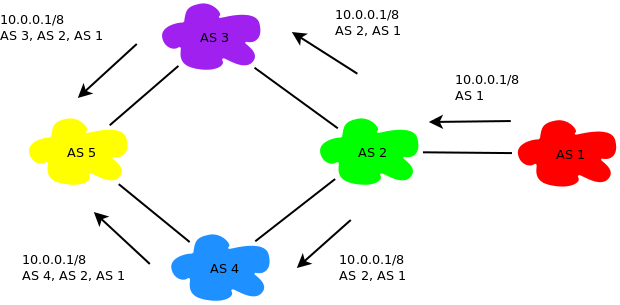
\includegraphics[scale=0.5]{bgpAdvertisement.png}
\caption{BGP Advertisement}
\label{fig:bgpAdvertisement}
\end{figure}

One vulnerability is that BGP does not ensure that a BGP-speaking router making the advertisement for on AS uses the AS number that this AS holds, neither ensures that the AS holds the prefixes it is advertising. As long as the neighboring router accepts the routes, a router can be configured to advertise routes into BGP with any AS number or for any destination prefix, including very small blocks (/30) or address blocks it does not hold. It is possible for the neighboring router to reject such cases, but it needs to be configured for that, meaning that a prior knowledge of acceptable prefixes and prefix lengths is needed. This makes the routing system quite vulnerable to misconfiguration or malicious attacks. The action of an AS advertising an unassigned prefix or belonging to another AS is know as prefix hijacking. When neighboring ASes receive this advertisement they might select the route and direct traffic towards this AS, as well as advertise this BGP route to their own neighbors. In Figure \ref{fig:bgpMaliciousAdvertisement} that AS 1 is advertising route 10.0.0.0/8 and it is the holder of this prefix. If AS 5 starts advertising the route to 10.0.0.0/8 and its neighbours select the shortest path routes, AS 3 and AS 4 will start diverting its traffic with 10.0.0.0/8 destination towards AS 5.

\begin{figure}[!h]
\centering
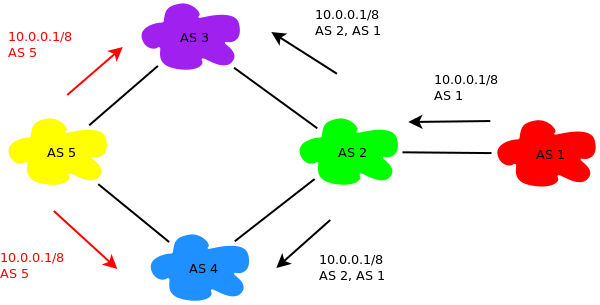
\includegraphics[scale=0.5]{bgpMaliciousAdvertisement.png}
\caption{BGP Malicious Advertisement}
\label{fig:bgpMaliciousAdvertisement}
\end{figure}

In the case that the offending AS just drops all packets destined to the hijacked addresses, the effect is known as a black hole, where the destinations seem unreachable to the parts of the Internet affected by this prefix advertisement. In the case that the AS decides to direct the traffic to hosts under its control the effect can be more severe, as the they can pretend to be the service provided by the hijacked destination. In this situation the traffic received by the AS can be analyzed and sensitive information, such as passwords or credit-card numbers, can fall in the wrong hands. It can also happen that the prefix hijacking is used to analyze the traffic before forwarding it to the correct destination, which would be a breach in the user's privacy. In order for an AS to do such an hijacking attack, it could advertise more specific prefixes then the ones in the original block (e.g., 10.1.128.0/17 and 10.1.0.0/16). This would work because of the longest prefix match rule used by IP routers, that forward packets to the more specific address range. In Figure \ref{fig:bgpDeaggregationAdvertisement} we can see an example. By advertising a more specific prefix (10.0.0.0/9), AS 5 will receive the traffic that had destination to AS 1.

\begin{figure}[!h]
\centering
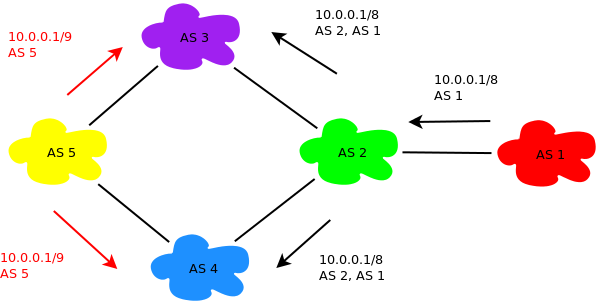
\includegraphics[scale=0.5]{bgpDeaggregationAdvertisement.png}
\caption{BGP Deaggregation Advertisement}
\label{fig:bgpDeaggregationAdvertisement}
\end{figure}


Routers exchange BGP announcement and withdrawal messages by establishing a BGP session with a pair. The BGP session runs over a TCP (Transmission Control Protocol) connection, which provides a reliable way to deliver a stream of ordered bytes, providing error correction and retransmission. BGP neighbors often have a direct physical link at the IP layer, but it can happen that they might have to communicate through an intermediate device. when a BGP session is extablished between ASes it is called an external BGP (eBGP) session, if the session occurs between routers in the same AS it is called an internal BGP (iBGP) session. This last type of sessions happen so that BGP routes learned from neighbors are spread throughout the AS. The communication between two BGP-speaking routers is also vulnerable to attacks, such as attacks against confidentiality, attacks against message integrity and denial-of-service attacks.

Besides being connected through physical links ASes are also bound by business or organizational relationships. An AS can serve as a provider to another organization and therefore there are contractual agreements, which are defined by service level agreements (SLAs). These agreements indicate the quality of service provided or define where the two ASes connect to each other and the traffic they will carry. For such reasons network operators need to be able to influenciate which BGP routes are chosen and which direct traffic will be accepted. For that they need to be able to specify routing policies. With BGP it is possible to enforce routing policies, such as forwarding data just for selected customers by using a number of protocol features. On of such features is the assignment of attribute values in UPDATE messages. BGP-speaking routers choose preferred routes by comparing the route attributes of the possible routes for each destination prefix. When network operators set specific fields in advance they can influenciate how route attributes are set. Among the most important BGP route attributes are local preference, AS path length, origin type and multi-exit discriminator (MED).

As mentioned, BGP routers can can be configured with route attributes in order to influentiate the route that is chosen. This allows to filter received (import policy) and advertised routes (export policy) to its neighbors while choosing where to forward its traffic. The problem is that the way an AS selects routes can be manipulated by sending BGP route announcements with bogus attributes. The AS-path attribute could be truncated to look shorter and therefore more attractive or add additional AS hops at the end. An AS could remove a particular hop from the AS path to modify traffic through certain ASes, or may add an AS number to the AS path so the the target AS would delete ith own AS number thinking it was a loop. An AS could also try to attach MED values to the routes to try to influentiate the route decision. 

One way to achieve a more reliable routing is by using the Routing Registries, which will be explained later in more detail, but their purpose is to provide a shared and global view of routing information. With an accurate routing registry of prefix ownership, AS-level connectivity and routing policies ASes could easily detect and discard invalid routes.  

After looking to how packets are forwarded in the Internet, the question that follows is how are IPv4 prefixes and AS numbers assigned. To that effect we will have a closer lookg to the Internet Assigned Numbers Authority and Regional Internet Registries.

\section{IPv4 Address Distribution}

In a communication protocol context, an address is an unique identifier used to distinguish between active elements, so that the protocol can provide the necessary support to enable communication between endpoints of the network defined by the operation of the protocol. In the Internet protocol context, an "IP address is an unique identifier that is assigned to a computer's interface running the internet protocol and connected to an IP network. The IP address has a minimal internal structure, which is a division into a network part and a host part. All hosts connected to a common network share the same value of the network part of their address, and uniquely identify themselves by the unique host part of the address. Currently there are two types of IP addresses in use: IP version 4 (IPv4), and IP version 6 (IPv6). IPv4 was deployed in January 1983 and is the most commonly used version. IPv6 addresses are 128-bit numbers and are expressed as hexadecimal strings, such as 2001:0ab2:3b3::56 and it started to be deployed in 1999. Although it was created to replace IPv4, it's full deployment is advancing slowly. 
To ensure that these addresses are unique there is the need of an organization responsible for delegating addresses and coordinating the Internet Protocol address system. 

\subsection{Internet Assigned Numbers Authority}

The Internet Assigned Numbers Authority, also known as IANA, is responsible for the global coordination of the Internet Protocol (IP) address system and also of the Autonomous Systems Numbers which are used for routing traffic on the internet.  

\begin{figure}[!h]
\centering
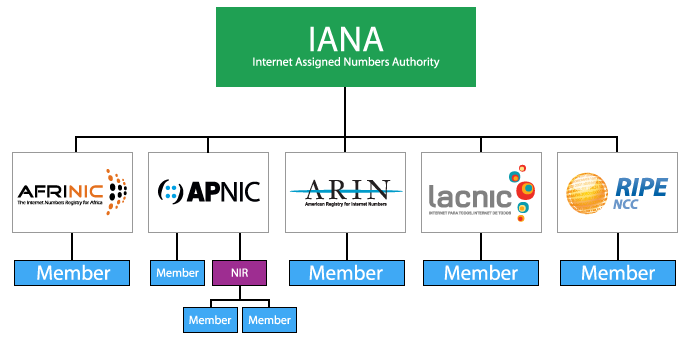
\includegraphics[scale=0.5]{IR-structure-diagram.png}
\caption{Global Structure of the Internet Registry System, source:\cite{FIG_GLOBAL_IRS}}
\label{fig:ir_structure_diagram}
\end{figure}

IP addresses are assigned in hierarchical manner as shown in Figure \ref{fig:ir_structure_diagram}. Internet Service Providers obtain allocations of addresses from a Local Internet Registry (LIR), a National Internet Registry (NIR) or from the corresponding Regional Internet Registry (RIR) and in turn they assign IP addresses to end users. IANA's main purpose is to allocate IP addresses from pools of unallocated addresses to the Regional Internet Registries according to their needs. IANA does not make allocation of IP addresses directly to ISPs or users except for allocations of multicast addresses or protocol specific needs. If a RIR requires further IP addresses for allocation, IANA makes an additional allocation to the RIR. There are five RIRs, each one responsible for a specific region: AFRINIC for Africa Region, APNIC for Asia Pacific Region, ARIN for North America Region, LACNIC for Latin America and the Caribbean Regions, RIPE NCC for Europe, Middle East and Central Asia Regions. The five RIRs are represented in Figure \ref{fig:rirs_image}.

\begin{figure}[!h]
\centering
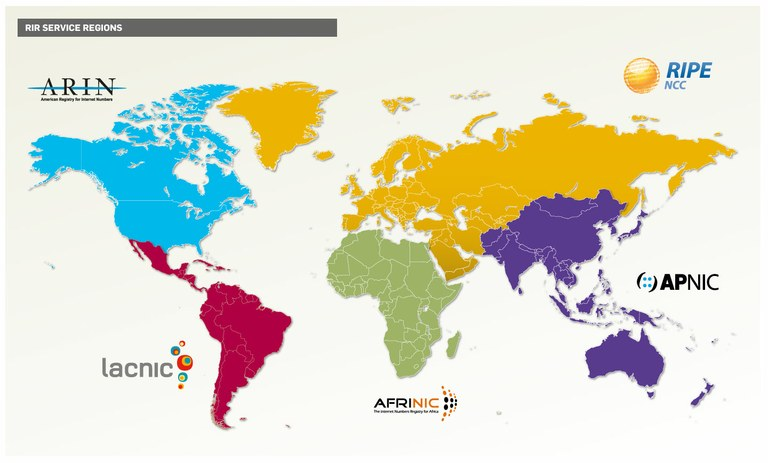
\includegraphics[scale=0.5]{RIR.jpeg}
\caption{Regional Internet Registries Service Regions, source:\cite{FIG_GLOBAL_IRS}}
\label{fig:rirs_image}
\end{figure}

Before the Regional Internet Registries (RIRs) were created, large blocks of addresses were given to universities, corporations and ISPs by the National Science Foundation. These addresses are nowadays administered by the individual RIRs. These early allocated IPv4 blocks of addresses are referred to as "legacy" blocks and the holders of these blocks are called "legacy holders". In \cite{IANA_Address_Space} we can see the IPv4 blocks distribution.


\subsection{Regional Internet Registries}


Among the tasks of a RIR are the coordination and representation of the members in its region. RIRs work together in order to develop consistent policies and promote best current practice for the Internet. As mentioned before RIRs are also responsible for allocating and assigning IP addresses within their respective regions. 

Local Internet Registries (LIR) are  established under the authority of a RIR and are responsible for the distribution and registration of address space at a local level. LIRs also ensure that resource allocation policies from RIRs are followed at a local level. LIRs are essentially members of a RIR and are normally operated by Internet Service Providers, but can also be large corportaions, governments and regulators.

The Internet Registry IP Allocation Guidelines were described in \cite{RFC_2050}, which became obsolete with the introduction of \cite{RFC_7020}. The objective of this document is to provide information about the Internet Numbers Registry System used in the distribution of globally unique Internet Protocol (IP) address space and autonomous system (AS) numbers and not to propose changes to the current system. Internet number resources are distributed according to three main goals: Allocation Pool Management; Hierarchical Allocation and Registration Accuracy. The goal of Allocation Pool Management is to allocate number resources in accordance to the needs of those running networks, but takink into consideration pool limitations when allocating. This is relevant as the pools from which IP addresses and AS numbers are allocated are finite. Hierarchical Allocation refers to the need of allocating IP addresses in a way that permits their aggregation into a minimum number of routing announcements, in order to ensure continued scaling of the Internet's routing system. The last goal, Registration Accuracy,  requires that a registry of allocations is maintained in order to provide accurate registration information of allocations and ensure uniqueness. This way it is ensured that IP addresses and AS numbers are not allocated to more than one organization.  

After the allocations are made, the allocated prefixes need to be advertised on the internet in order to have reachability. As mentioned before, in order for an IP prefix to be reachable, it needs to be advertised in the Internet and the protocol responsible for this is BGP. At a global level, this means that thousands of routers need to be configured to ensure reachbility. To make this process less painful the Internet Routing Registries were created, which should work as a global repository of announced routes and routing policies so that backbone routers could be easily configured. 

\subsection{Internet Routing Registries}

The National Science Foundation inherited the responsability for developing the U.S. Internet from the Advanced Research Projects Agency (ARPA) and the Internet Routing Registry concept goes back to the 1980's and to the National Science Foundation Network (NSFNet).  NSFNET refers to the program sponsored by the National Science Foundation, initiated in 1985, with the purpose of support and promote advanced networking among U.S. research and education institutions. Among its participants were Merit Network, Inc., IBM, MCI, Advanced Network \& Services, Inc., the State of Michigan and many institutions in research and education. As a way to configure the MSFNET's backbone routers, the Policy Routing Database (PRDB) was used since 1989. Merit planned the retirement of PRDB for December 1994, which would be replace by the Routing Arbiter Database (RADB). RADB would then become part of the Internet Routing Registry (IRR) along with RIPE NCC, MCI and other registries. The IRR objective was to be a global public repository of announced routes and routing policy in a common format so that ISPs could use this information to configure their backbone routers and analyze routing policy.

\begin{figure}[!h]
\centering
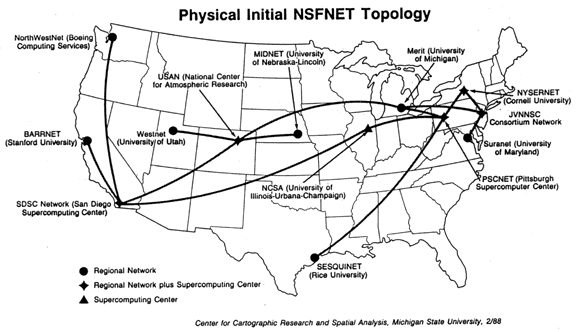
\includegraphics[scale=0.5]{nsfnet_topology.png}
\caption{NSFNET Topology, source: \cite{NSFNET_Topology}}
\label{fig:nfsnet_image}
\end{figure}


PRDB goal was to maintain information regarding legitimate destination announcements from the various regional networks. This information was very important in order to prevent routing loops. Only after BGP replaced EGP as the inter-domain routing protocol, it became no longer necessary to controll the avoidance of routing loops in such a administratively way. With this change, the information in PRDB turned to be mainly used to gather routing policies, such as path preferences and to generate configuration files for backbone routers.

With the transition of NSFNET to the commercial Internet, the National Science Foundation selected Merit Network and a partner organization to act as Routing Arbiters. The goal of the PRDB would be now to record global routing policy information based on each Autonomous System's policy and RADB comes into the scene. RIPE had pioneered work to record global routing policy information in Europe and the data exchange format described in RIPE-181 \cite{RFC_1786} was adopted as the standard for Internet Routing Registries. This model was also taken by RADB. 

The transition from PRDB presented several problems as the tools used to configure the NSFNET/ANSnet routers were based on PRDB attributes and not RIPE-181. But by December 1994, all the data in PRDB had been converted to RIPE-181-style expressions and on February next year, the RADB had been populated with RIPE-181-style Maintainer and AS Objects. Later this format shifted to the Routing Policy Specification Language (RPSL), which is currently used. In Appendix A can be found more information on the most relevant objects and the changes from RIPE-181 to RPSL.

Nowadays the Internet routing Registry (IRR) is a globally-distributed routing information database. This set of databases consists of around 34 different databases, each one individually operated by organizations such as RIRs (ARIN, RIPE, etc), ISPs (NTT, Savvis, Level3, etc) and non-affiliated public registries (RADB and ALTDB). RADB is just one component of the IRR, but its goal is to mirror all component databases and provide an overview of the entire IRR. 

The purpose of the IRR is tho provide a tool where network operators publish their routing policies and routing announcements so that other network operators can use this information. It allows them to debug routing problems, configure backbone routers automatically and do network planning. 

Using the IRR provides several advantages to networks. The fact that IRR hods announced routes and routing policies in a common format, allows network operators to use this to configure their backbone routers. This helps network management in route filtering, where traffic can be filtered based on registered routes, thus avoiding network problems caused by malicious or accidental routing announcements. It can also be used for network troubleshooting by making easier to identify routing problems outside of ones network and allowing to use the contacts for the AS number associated with the problematic route in order to solve traffic problems. IRR also makes easier to create router configurations by using tools such as IRRToolset. In case that all networks would register their routes in the IRR, a global view of routing policy could be mapped, thus improving the integrity of global Internet routing. 

This IP address space management system has been working well, but currently we are facing the problem of IPv4 address exhaustion, which will be referred in the nex section.

\section{IPv4 Address Exhaustion}

Since the 90s that the technical community knows that the use of IPv4 could not scale in a global deployment containing vast concentrations of communicating devices, due to the fact that IPv4 is limited to 4 billion addresses. To tackle this, IPv6 was created. Its technical specification was completed by 1996 and at this time it was initiated a programme to promote the need to transition from IPv4 to IPv6 before the anticipated exhaustion of the IPv4 address pool. The major challenge to achieve this is that IPv6 is not backward compatible with IPv4, meaning that we cannot just replace IPv4 with IPv6. End devices, networks and service delivery points need to be able to support both protocols simultaneously and be able to provide a dual protocol capability before the IPv4 component of the network is taken out of service.     

As reported in \cite{IPv6_state}, the transition to IPv6 is still in an early stage, while the Internet faces an accelerated growth with the deployment of more and more connected devices, where almost any new device tends to be connected to it.  This evolution has put pressure on the supply of IPv4 and we assisting to a state of IPv4 address exhaustion. At the same time the transition to IPv6 has not been following a rapid deployment. The hope at the time of the specification was that service providers would prevent the exhaustion of IPv4 addresses and switch to an all-IPv6 network before the pool of IPv4 addresses was depleted. Unfortunately this didn't happen and in February 2011 the pool of IPv4 addresses administred by the Internet Assigned Numbers Authority (IANA) was fully allocated. Two years after, by August 2013, two Regional Internet Registries, APNIC and RIPE, reached a critical low number of managed IPv4 addresses. Nevertheless, the overwhelming majority of end users and services on the Internet continues to rely on IPv4. This implies that the transition to IPv6 needs to be planned as a dual-stack transition, starting from an exclusive model of just using IPv4 to a dual protocol stack mode.

One reason of the reasons for the delay in deploying IPv6 lies in the supply chain for the Internet's service provider sector. The integration of support for IPv6 in the service provider and customer equipment has taken many years. Another reason is the large scale use of Network Address Translation (NAT) by service providers. NAT is placed at the edge of a network and allows multiple devices inside to share a single exterior public address and it has become a common model for Internet service deployment on wired networks. 

The current statistics on address distribution are shown in \ref{fig:rirs_available_ipv4}.

\begin{figure}[!h]
\centering
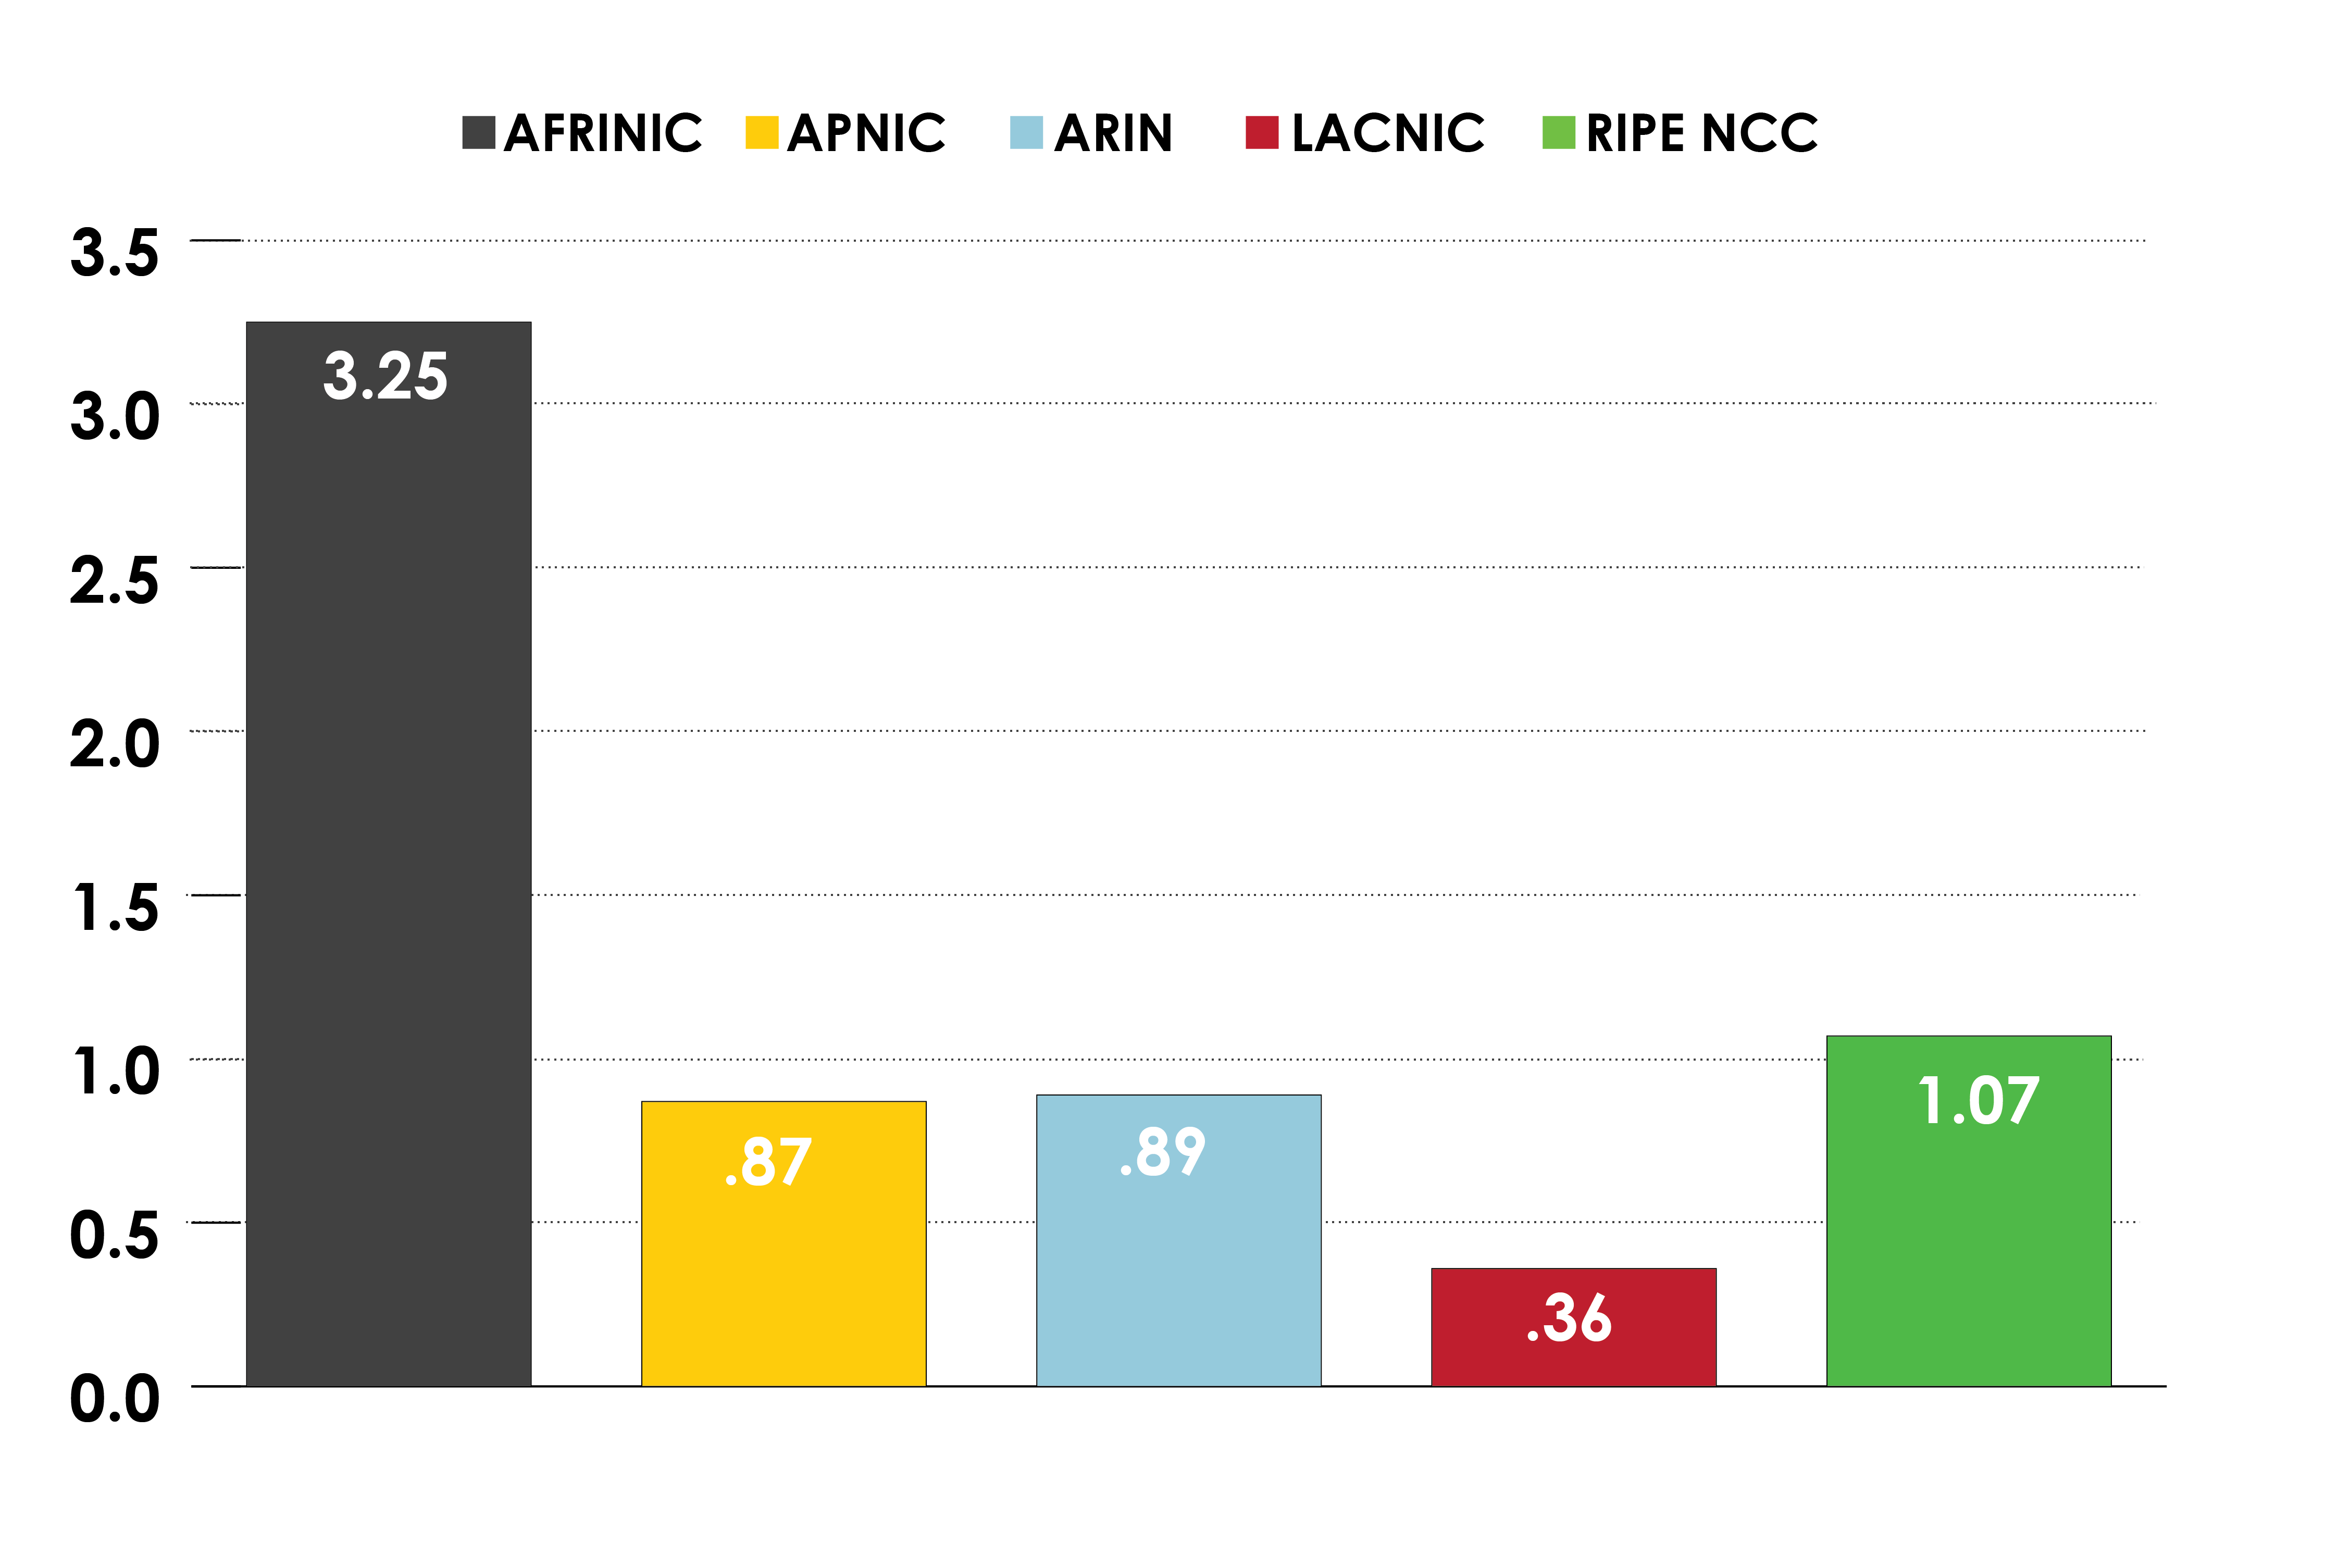
\includegraphics[scale=0.3]{ipv4inRir.png}
\caption{AVAILABLE IPv4 /8s IN EACH RIR, source:\cite{IPv4_EACH_RIR}}
\label{fig:rirs_available_ipv4}
\end{figure}

We can see that only AFRINIC still has 3.2 /8s, RIPENCC 1.07 /8s where all the other registries have less that 1 /8 block of addresses. This indicates how low is the current size of the pool blocks of IPv4 addresses in each RIR. To face this problem the Regional Internet Registries changed the allocation policies. The first RIR to reach a conclusion of the general address allocation function for IPv4 addresses was APNIC, on April 2011. Since then, APNIC is operating its IPv4
allocations under a "Last /8 Policy" \cite{APNIC_last8} where each entity may apply for one, and only one, allocation of up to 1024 addresses. The intent of this policy is to hold onto a small pool of addresses to assist new entrants in the area of Internet Service Provision to operate in dual-stack mode with some a small amount of IPv4 for their IPv4 dual-stack needs. The second RIR to also run to the end of its general address allocation policies has been the RIPE NCC, which exhausted its pool on 14 September 2012. The RIPE NCC has also moved into a framework of a Last /8 Policy \cite{RIPE_last8} with similar constraints in place in APNIC. 

When a local registry or an ISP gets addresses assigned, they can use it in a number of ways. If the address is used for interactions with the public Internet, this address has to be advertised on the routing system. Each individual routing annoucement covers a range of addresses and it doesn't mean that all of these addresses are uniquely assigned to an end device, but normally it is considered that the announcement of a network prefix indicates that the addresses included are being used in some way. Addresses can also be used for some other purpose besides the public Internet, so if one address is not being advertised in the Internet's routing system, it does not a clear indication that it is not being used in an active network.

Due to the fact that many assigned IPv4 addresses might not be being used, it has been discussed within each reagion the possibility of trying to reclaim these addresses. This has several issues for the registries as the agreements between them and the address holders do not oblige the address holders to immediately advertise the assigned addresses on the public Internet and these addresses can also be used in a context where they are not advertised on the public Internet. There is also the case where blocks of addresses were distributed before the creation of the RIR's, called legacy blocks, where there are no formal obligation on the address holder. There has been cases where the responsible RIR has been able to reclaim addresses, specially due to the fact that the address holder didn't fulfill his obligation with respect to the agreement between the parts involved, but the total number of addresses reclaimed had no real impact in the address runout issue.

Another way to reutilize IPv4 address space is to allow organizations holding IPv4 addresses to sell address blocks to other organizations interested in bying them. The IP address transfer markets could be a way to extend the life of the IP address space. One major benefit of this type of market could be to offer an incentive for address space holders to release unused address resources. An open and legitime transfer market would, as mentioned before, give an incentive to reclaim unused address space, but could also help in a better and accurate registration and administration of address space instead of a gray or black IPv4 address market. A better and accurate registration and administration would benefit Internet security.  

The fact is that the IP address transfer market can no longer be denied, specially after the deal in which Microsoft bought Notel's address space assets. Either because people believe there should not be a fee for such a resource or because the the transfer market might delay the migration to IPv6, many in the Internet technical community still feel skeptical about it. The truth is that it is difficult to have a comprehensive picture of this market, because the IP number allocations is controlled by five separate regional registries, each one with different databases, disclosure practices and different policies regarding transfers. 

In particular we are interested in studying the effects of IPv4 address exhaustion in on allocation and routing dynmics.

\chapter{Related Work}

The related work for this study includes a number of BGP and Internet routing measurement studies. Some of these studies focus on address allocation patterns and the impact on routing table growth \cite{Impact_Structure_Routing_Tables}, \cite{Slowing_Routing_Table_Growth} and \cite{BGP_Routing_Table_Evolution}.

In \cite{MOAS} were analized the BGP multiple Origin AS conflicts. It was observed the most of the conflicts were short-lived, lasting only a small number of days and could happen due to multi-homing without BGP and advertising routes to exchange points. It could also happen due to router misconfigurations. These types of conflicts were associtated to large scale network outages and other problems. 

In \cite{Address_Space_Deaggregation} it is analized the address space deaggregation and it is found that there is no trend towards more aggressive prefix deaggregation or traffic engineering over time. Also the results show that the global impact of "bad guys" on Internet space deaggregation has not changed for worse and these problems have been present for a long time.

In \cite{Comparative_BGP_IRR} it is carried out a extensive analysis of IP prefix and origin AS pairs in BGP against the information registered with the IRR. The study showed that the registration of BGP PO pairs in the IRR is prevalent, which opens the door to build important services based on the IRR data.

\cite{Capturing_Ghosts} used a new statistical capture-recapture technique to estimate the used IPv4 address space from several sources of active and passive measurement data instead of a more common ICMP probe to infer address usage. The study indicated a 1.1 billion IPv4 addresses in use across 6.3 million /24 subnets and a growth of around 0.5 million /24 subnets and 160 million IPv4 addresses per year. It is referred that at this rate the remaining /24 subnets will be used by 2022.

In \cite{Delegation_Structure} is shown that the increase in the number of advertised prefixes is due to increase in allocations as well as in fragmentation and that the rate of growth of allocation and fragments are similar, which indicates that the rate of fragmentation as been constant.


In \cite{Land_Grab} and  \cite{IPv4_Transfer_Markets} take a look into the IPv4 transfer Markets. The first paper focus on the need of a proof of ownership for addreses in the form of resource certification. It is presented a way of using reverse DNS to achieve resource certification. The second paper analyzes address transfers that have been completed and found that 75\% of them involve underutilized prefixes and in general are advertised via BGP shortly after their occurrence. It was also observed an increasing trend in the number of transfers, but the number os transferred prefixes is still small.

In \cite{IPv6_state} it is discussed the state of IPv6 implementation as well as means to continue using IPv4.

One of the most important source of information is the Potaroo web page \cite{Potaroo}. 
Here we can see statistics regarding IPv4 address space allocation. There is information for each RIR regarding IPv4 address pool status, allocations made and the total span of address space advertised in the BGP routing table over time. It is also possible to obtain the delegation files for each RIR or a joint file.


\chapter{Datasets}

In order to study the advertised IPv4 address space we used BGP table dumps from RouteViews \cite{RouteViews}. This provided us the required raw BGP data for our analysis. As our requirements were just to have a global overview of the prefixes that are being advertised and its origin, to use only this data source would be enough. In case we had to infer about the BGP paths and try to build an internet map, we would certainly have to use more sources (e.g. BGP table dumps from RIPE), but for our analysis this was not necessary as we could obtain a comprehensive view of the global routing system.
We used four collectors, after some previous tests, which would give us the best possible overview of the global system for the entire study period. Some other related work \cite{Address_Space_Deaggregation} used just one collector and still obtained significant results, but we wanted to be on the sure side and decided to use four collectors. 

To be able to study the IPv4 address space allocation history, we used the allocation files \cite{Potaroo} provide by the RIRs. These files contain information about address allocation and are publiched in the RIR Statistics Exchange Format.
How Allocation Data is Published \cite{ALLOC_FILES}. Each RIR publishes a file containing its allocations. The files are CSV formatted using a pipe "\textbar" as field separator and have the following format:
\vspace{5mm}

\hspace{1cm}	 registry\textbar cc\textbar type\textbar start\textbar value\textbar date\textbar status [\textbar extensions...]
	
\vspace{5mm}

"registry" contains the name of the registry to which this IP is assigned to, "cc" is a two letter country code in the ISO 3166 format. "Type" can be "asn", "ipv4" and "ipv6" where asn is for Autonomous System Numbers and the other fields are for IP version 4 and version 6 respectively. "Start" is the starting IP address for the block and "value" is the number of hosts in this block. "Date" provides information to when this block was first assigned by the RIR. "Status" provides information to whether the block was assigned or allocated. "Assigned" are blocks that are allocated to the final instance using it and "allocated" are delegated to LIRs that in turn allocate the block in parts. An example would be:
\vspace{5mm}

\hspace{1cm}	 ripencc\textbar DE\textbar ipv4\textbar 193.168.128.0\textbar 32768\textbar 19960308\textbar assigned

\vspace{5mm}

We used the Whois \cite{Whois} query and response protocol used for querying databases to obtain information about a domain name, an IP address block and an autonomous system. 

We used Merit RADB \cite{RADB} which is a public registry of network routing information as an Internet Registries data source. The choice was to use RADB because its mission is to mirror all Internet Registries  databases to provide the most complete view possible of the entire IRR. 

\section{Data cleaning}
The RouteViews collectors contains the bgp information provided by the peer ASes. For our case study, most of the information is redundant. As we intend to analyze the prefixes that are being advertised and who is advertising them (origin), this information will be provided by most of the peer Ases. The first step to arrange our data and remove redundant information was to identify the most relevant peers. These would be the ones that would provide us the most complete view of the entire internet reagarding the number of prefixes that are advertising and how reliable they were throughout the entire time period of our analises. In Figure \ref{fig:peers1} it is shown all the information gathered from 2001 until 2014. 

\begin{figure}[!h]
\centering
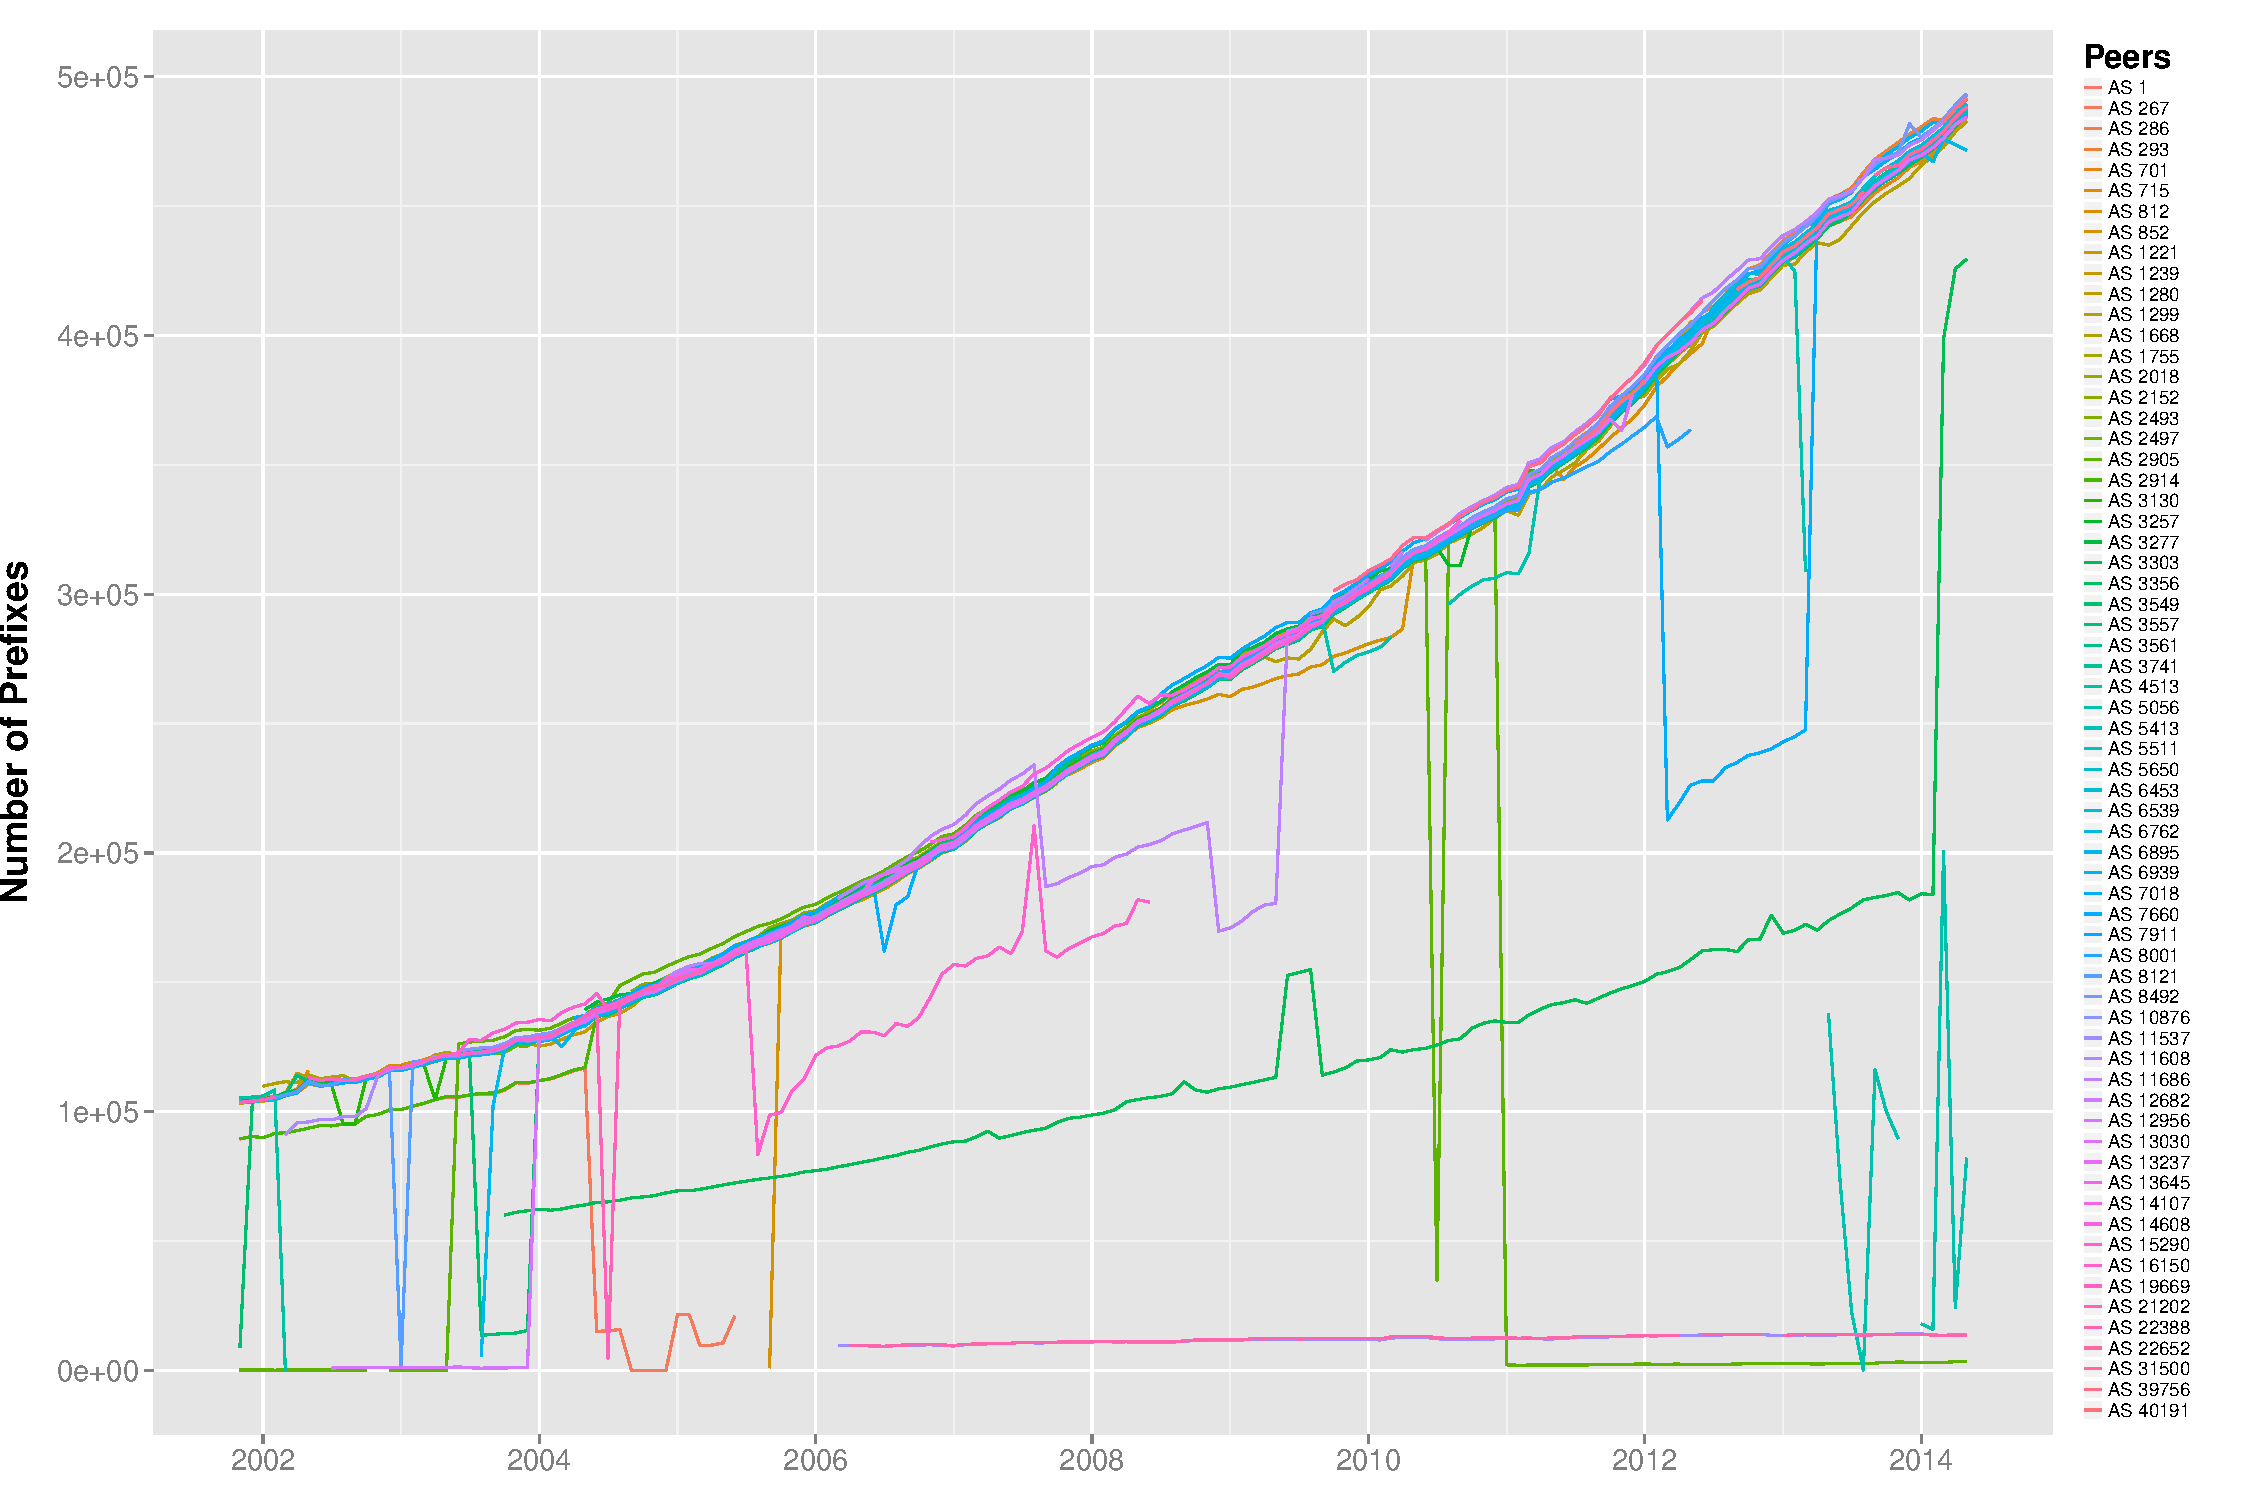
\includegraphics[scale=0.35]{peers1.pdf}
\caption{Peers 1}
\label{fig:peers1}
\end{figure}

It is possible to see that a great number of peers provide less information than others and also that a high number of peers don't provide information whitout breaks throughout the time period. We then procceeded to remove all the peers that delivered a lower number of advertised prefixes or that didn't deliver information at a determined point in time. The result is shown in Figure \ref{fig:peers2}.  

\begin{figure}[!h]
\centering
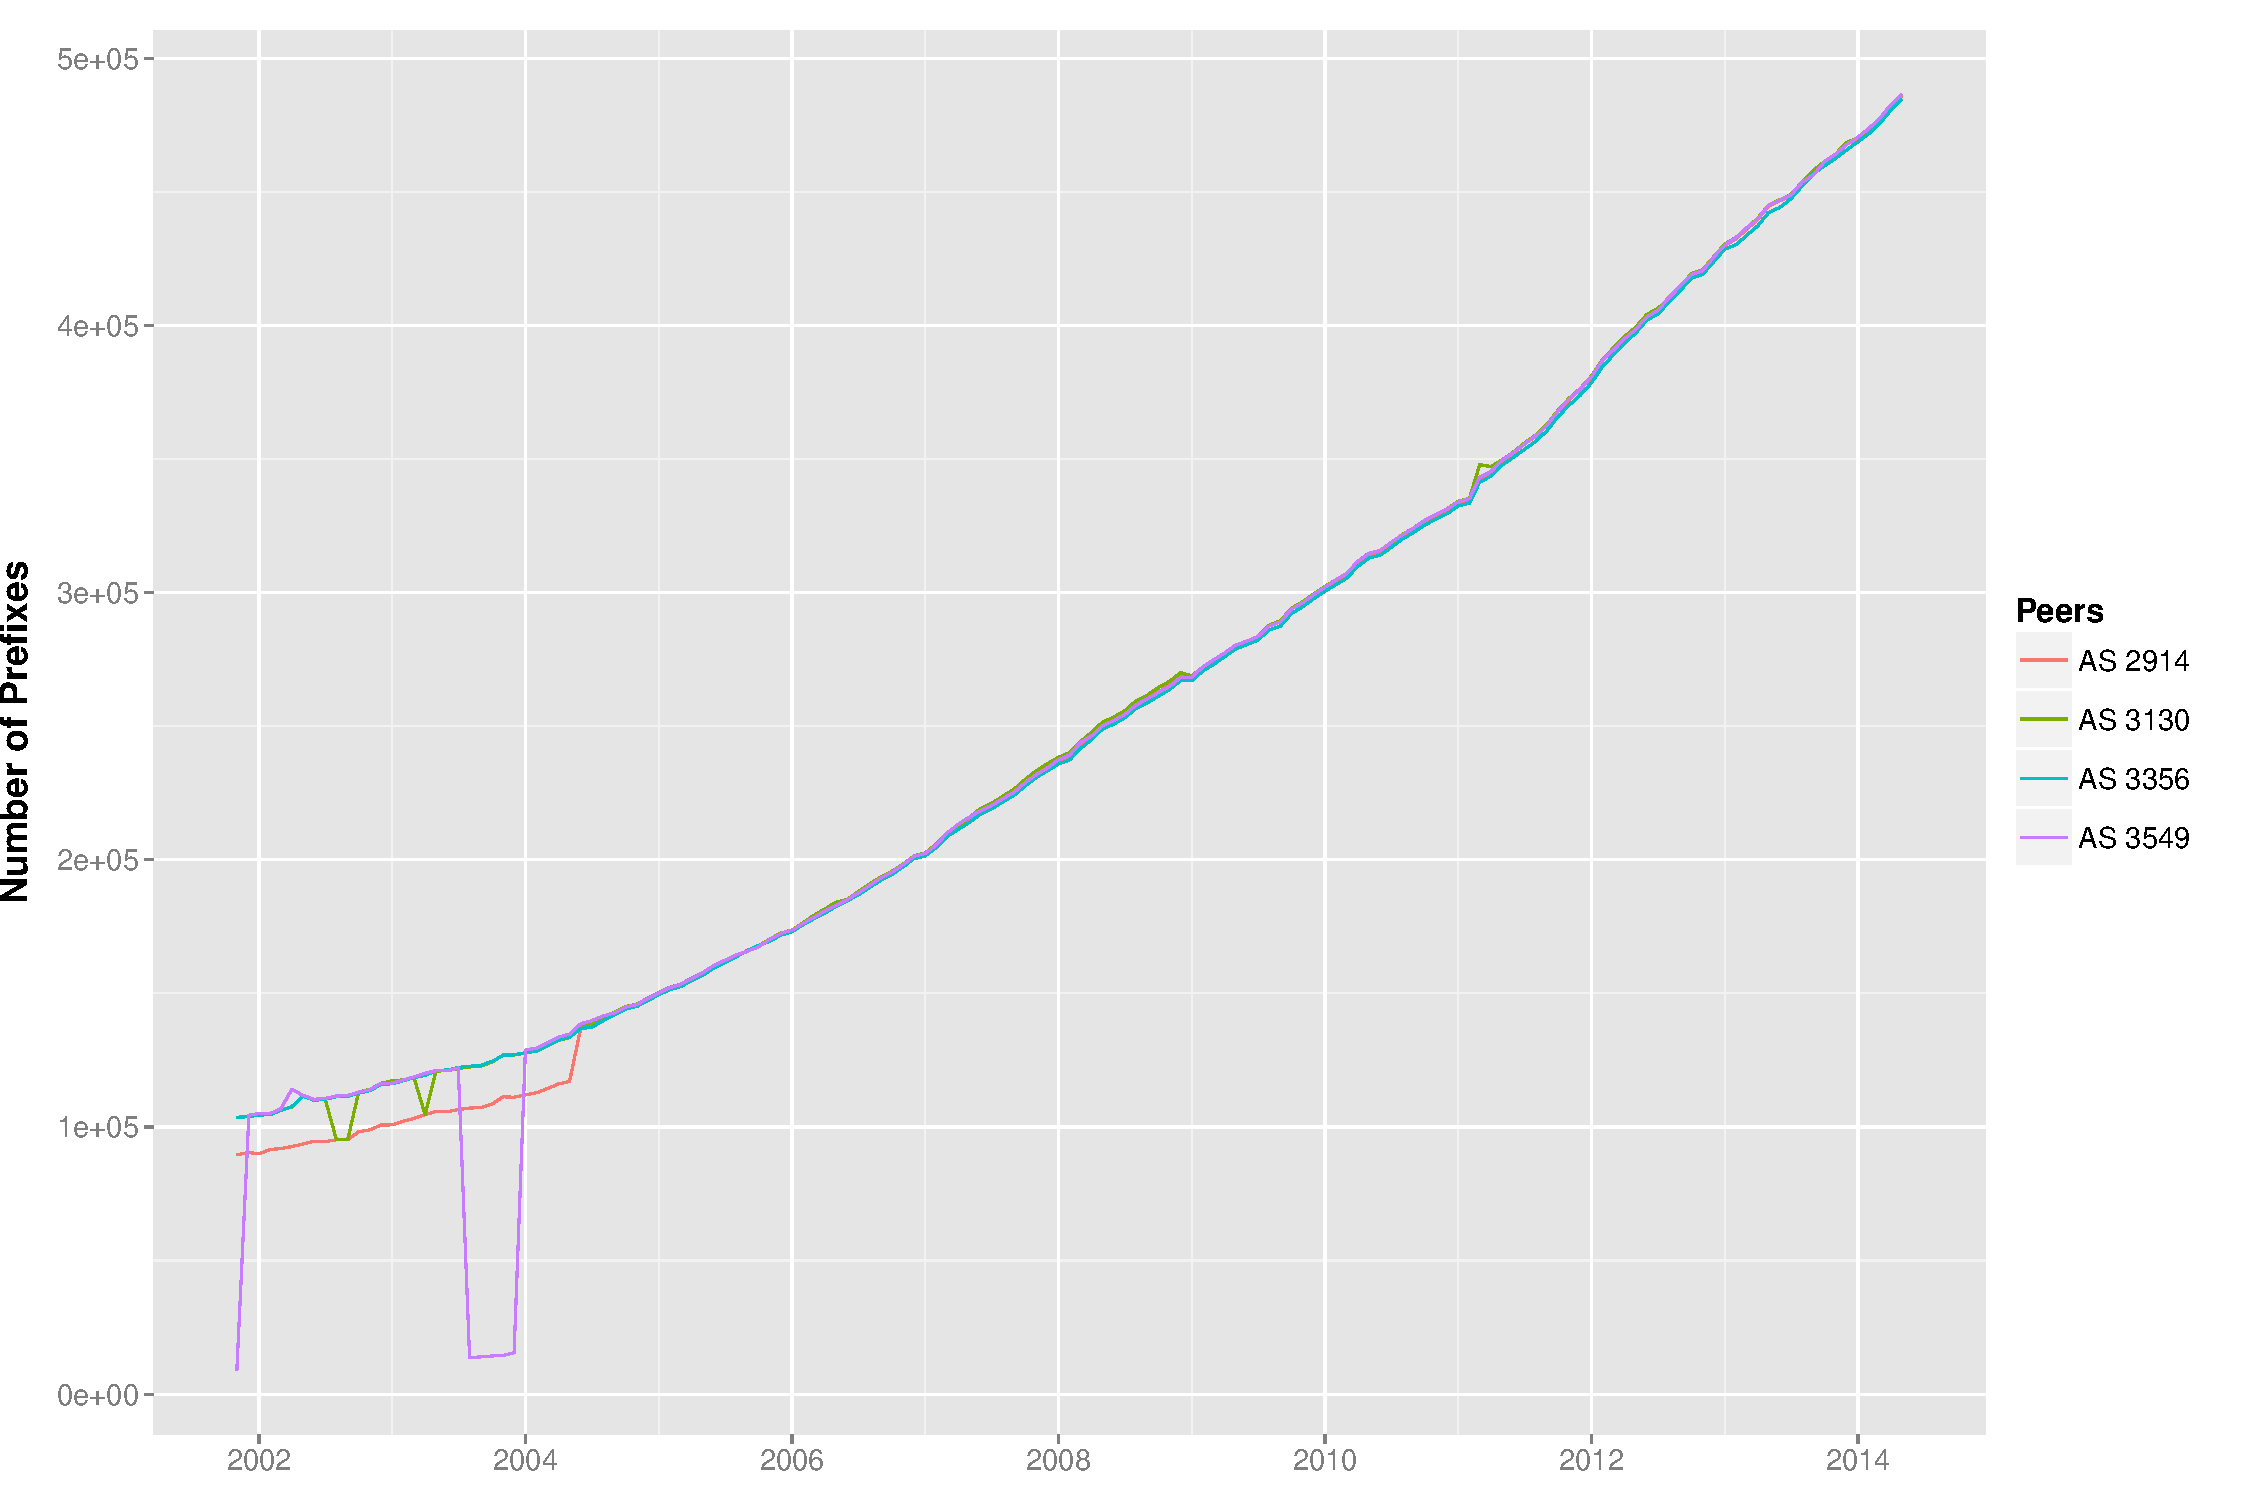
\includegraphics[scale=0.35]{peers2.pdf}
\caption{Peers 2}
\label{fig:peers2}
\end{figure}

By doing this we reduced drastically the amount of data that would have to be analyzed and at the same time we would have a dataset capable of ensuring the best possible data quality. 

\chapter{Analysis \& Results}


\section{BGP Origin Dynamics}

Our first approach was to analyze the number of prefixes that changed origin during the studied time period. We started by mapping, for every month, the advertised prefix in BGP data to its origin AS so that we would have a prefix-origin pair. Having this mapping we compared subsequent months and checked for each prefix if the origin changed. This gave us an origin-origin pair and everytime this pair had different values we counted it as one occurrence of origin-origin pair change. The results are shown in Figure \ref{fig:comparePrefixes}.

\begin{figure}[!h]
\centering
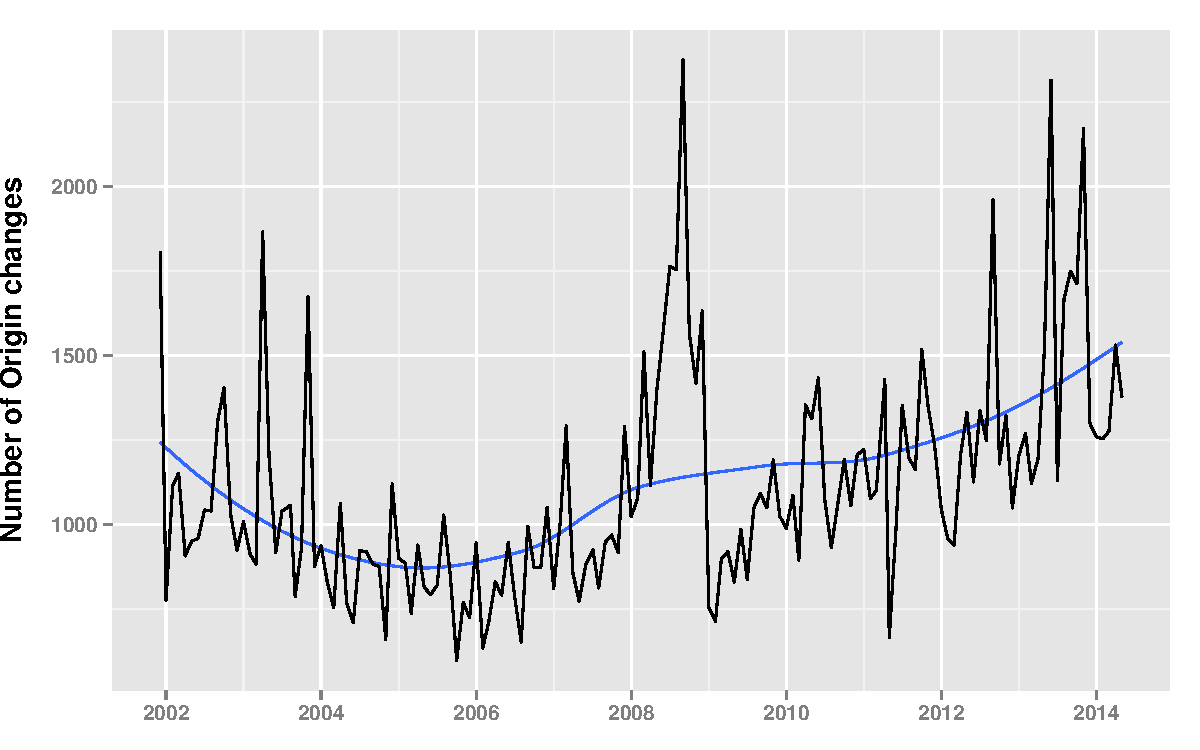
\includegraphics[scale=0.35]{comparePrefixes.pdf}
\caption{Observed number of monthly
origin-origin pair changes}
\label{fig:comparePrefixes}
\end{figure}

The first thing that we notice is that the data is very noisy and therefore we use the moving average to help us in our observation. We see that since 2002 until 2005 the number of origin-origin pairs, or prefixes that changed their origins, was decreasing and since then started an increasing tendency, showing a higher increasing rate since 2011. The fact that the number of prefixes being allocated by the RIRs has also been increasing along the time period could help to explain this increasing tendency, but we noticed that during the period between 2002 and 2005, and while the number of allocations was also increasing, the number of prefix origin changes decreased. Therefore there is not a positive relation between the number of allocations and the number of prefix origin changes. There are several reasons for a change of origin in a prefix \cite{IPv4_Transfer_Markets}, such as transfers, BGP misconfigurations or prefix hijacks and because the prefix moved between two ASes belonging to the same organization and to point out the direct cause for a prefix origin change is very difficult.      

By looking at the moving average we can see that in 2014 there were around 1500 prefix changes and when comparing to the number of prefixes in the BGP RIB table \cite{Potaroo}, which are around 500 000, we see that 1500 are just a small number of occurrences.

Our next step was to deaggregate every prefix found in BGP data into subnets of size /24 and map it to the origin AS. The end result was a prefix-origin mapping where each  prefix was a /24 subnet mapped to the AS advertising it. When deaggregating the prefixes and mapping them we considered always the most specific /24 subnet, this means that, for example, if AS1 advertises the prefix 10.0.0.0/8 and AS2 advertises the subnet 10.1.0.0/16 all the /24 subnets in 10.1.0.0/16 will be mapped to AS2 and the others subnets beyond this will be mapped to AS1. We then used this /24-origin mapping to compare subsequent months and check for each /24 if the origin changed. Everytime the /24 changed origin we counted as one occurrence. The results are shown in Figure \ref{fig:comparePrefixes_24}. 

By deaggreting the advertised prefixes into /24s we can get an idea of the size of the prefixes that change origins.  

\begin{figure}[!h]
\centering
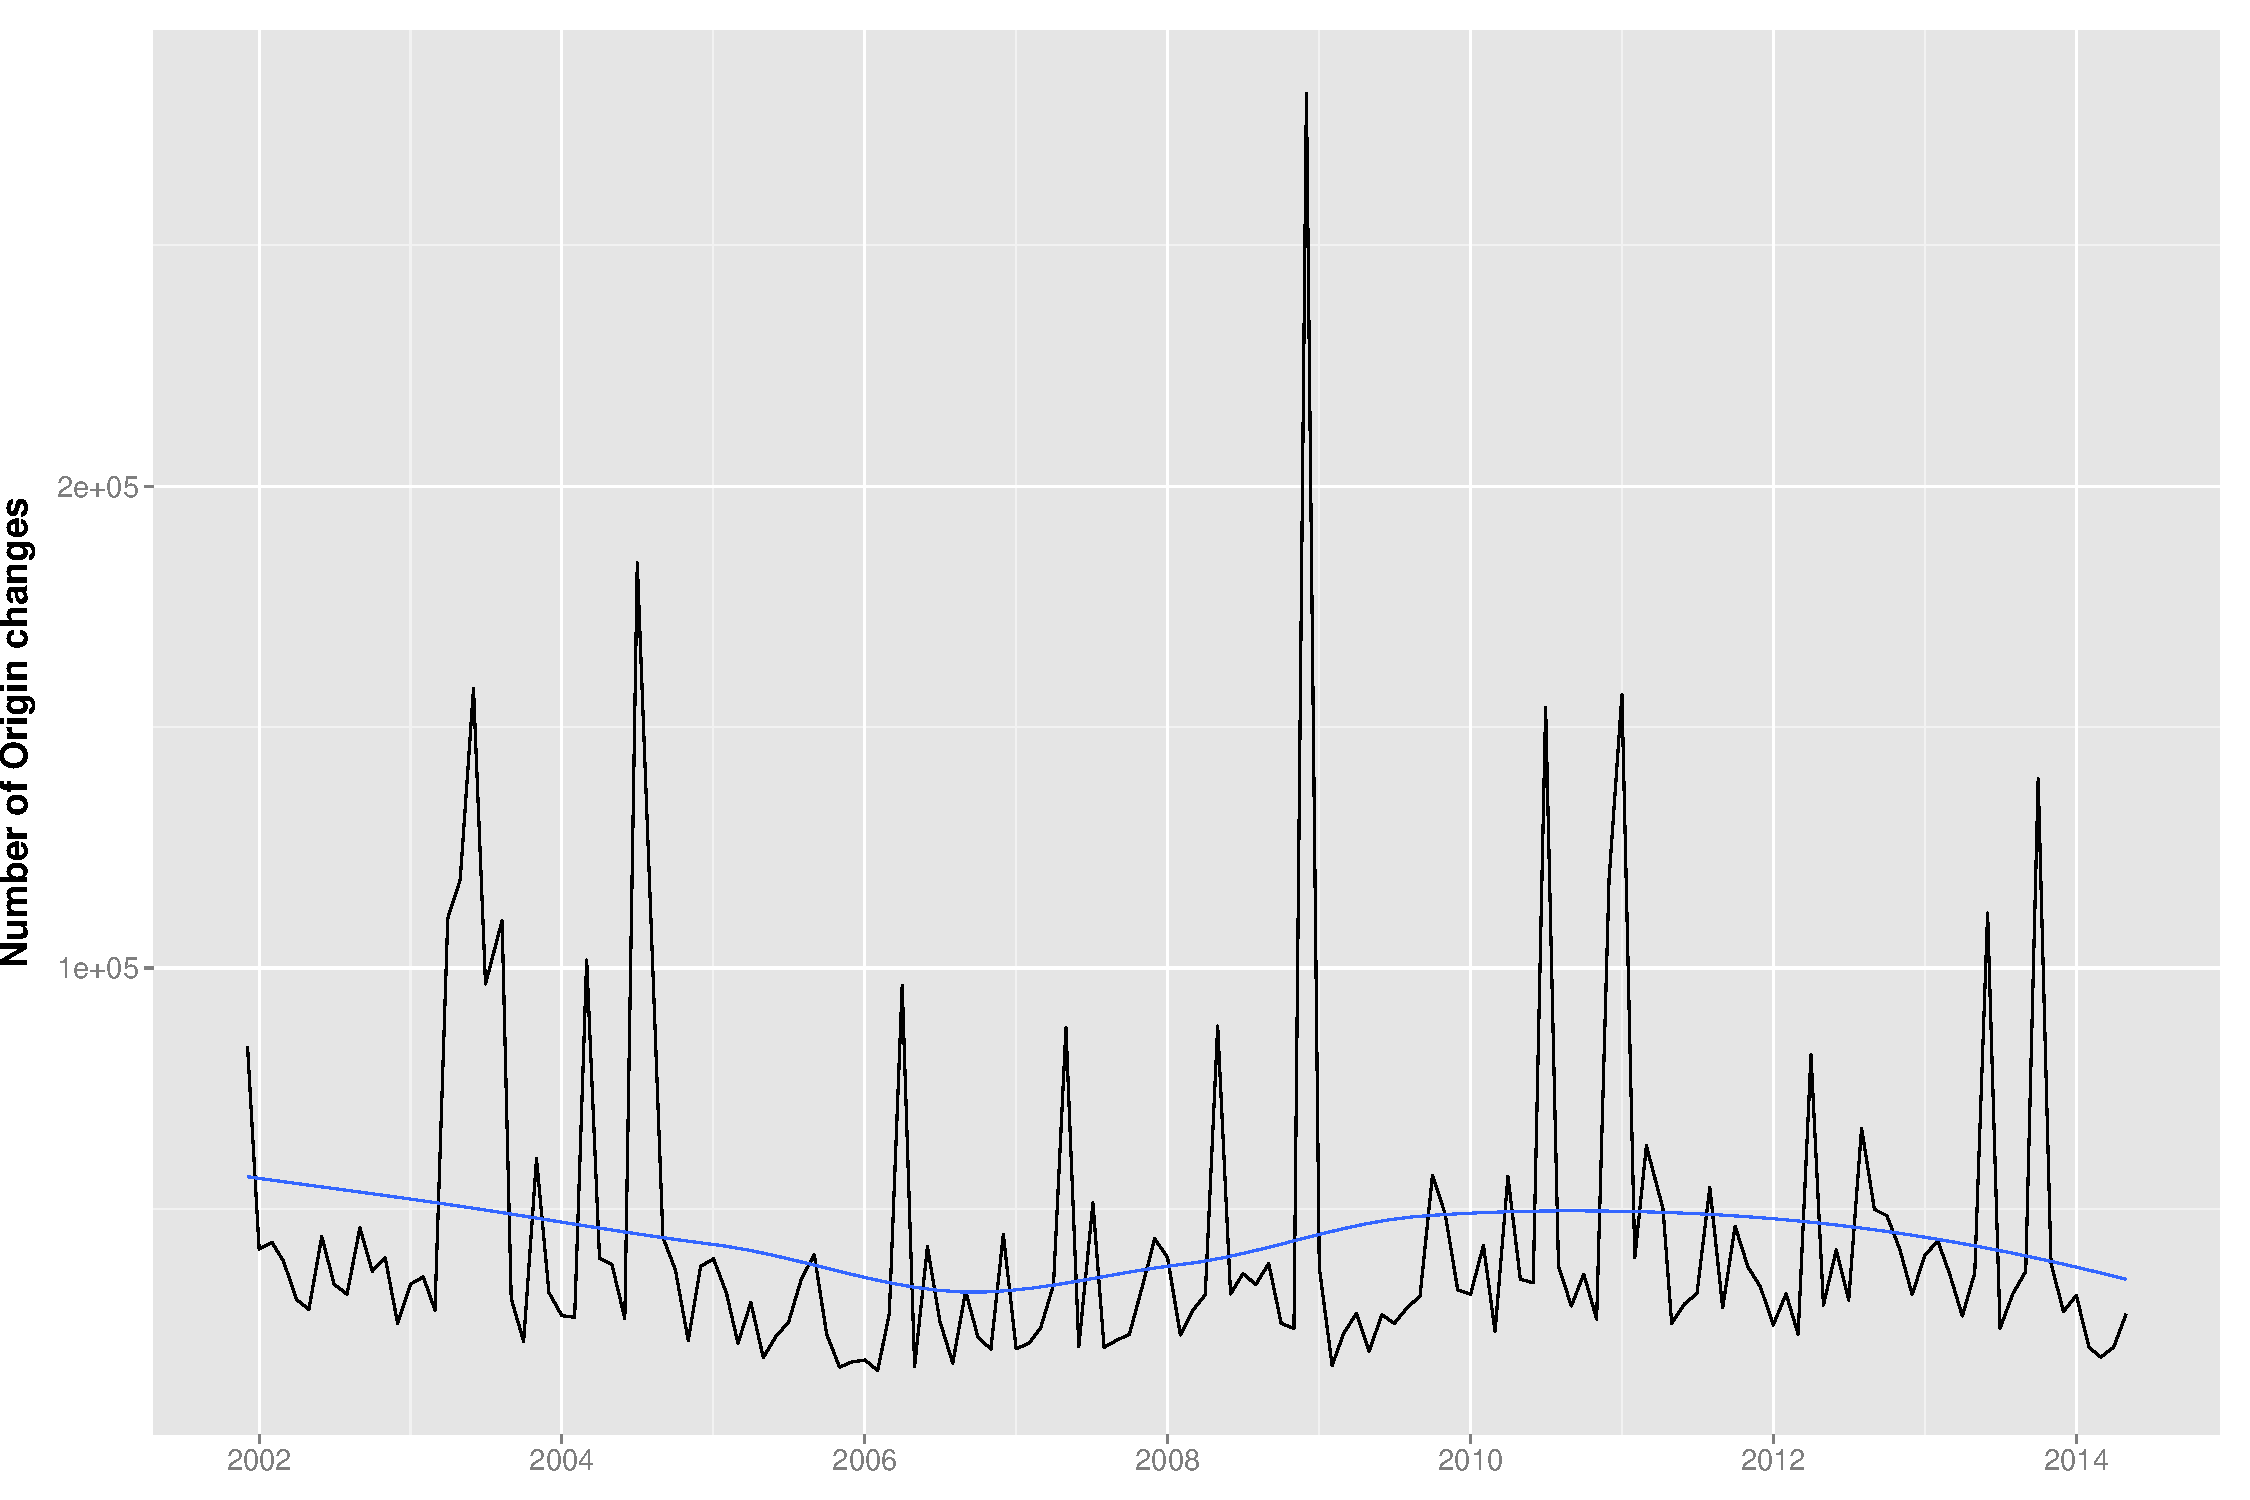
\includegraphics[scale=0.35]{comparePrefixes_24.pdf}
\caption{Observed number of monthly
/24s that change their origin}
\label{fig:comparePrefixes_24}
\end{figure}

We can see that when reasoning about /24 address blocks we cannot have a clear idea about the number of prefixes that changed origins, especially due to heavy-hitters such as /8 and /16 blocks of addresses. The best example is the peak around 2009 that indicates that one of those blocks changed origin. There are also smaller peaks, in 2003, 2004 as well as between 2010 and 2012 that indicate the same. 

By just looking at the moving average we see that the amount of subnets of size /24 that change origin along the time period didn't oscillate much, but we see that the Figure \ref{fig:comparePrefixes_24} is extremely noisy and it is difficult to infer on what it is really happening.






The next step was to aggregate the origin changes. For that we went back to our first mapping, where we mapped for every month, the advertised prefix in BGP data to its origin AS and obtain a prefix-origin pair. We then started comparing subsequent months and checked for each prefix if the origin changed. This gave us an origin-origin pair 
which we then grouped with the other pairs with the same origin-origin. Each of these groups would count as one occurrence. Considering the case where two prefixes 1.1.2.0/24 and 1.1.3.0/24 where both advertised by AS1 and in the next iteration they started being advertised by AS2, it would lead to the pair (AS1, AS2) for each of the prefixes. The result would be one occurrence for the grouped origins that we are considering. In Figure \ref{fig:compareAggregation} are shown the results when applying this metric.       

\begin{figure}[!h]
\centering
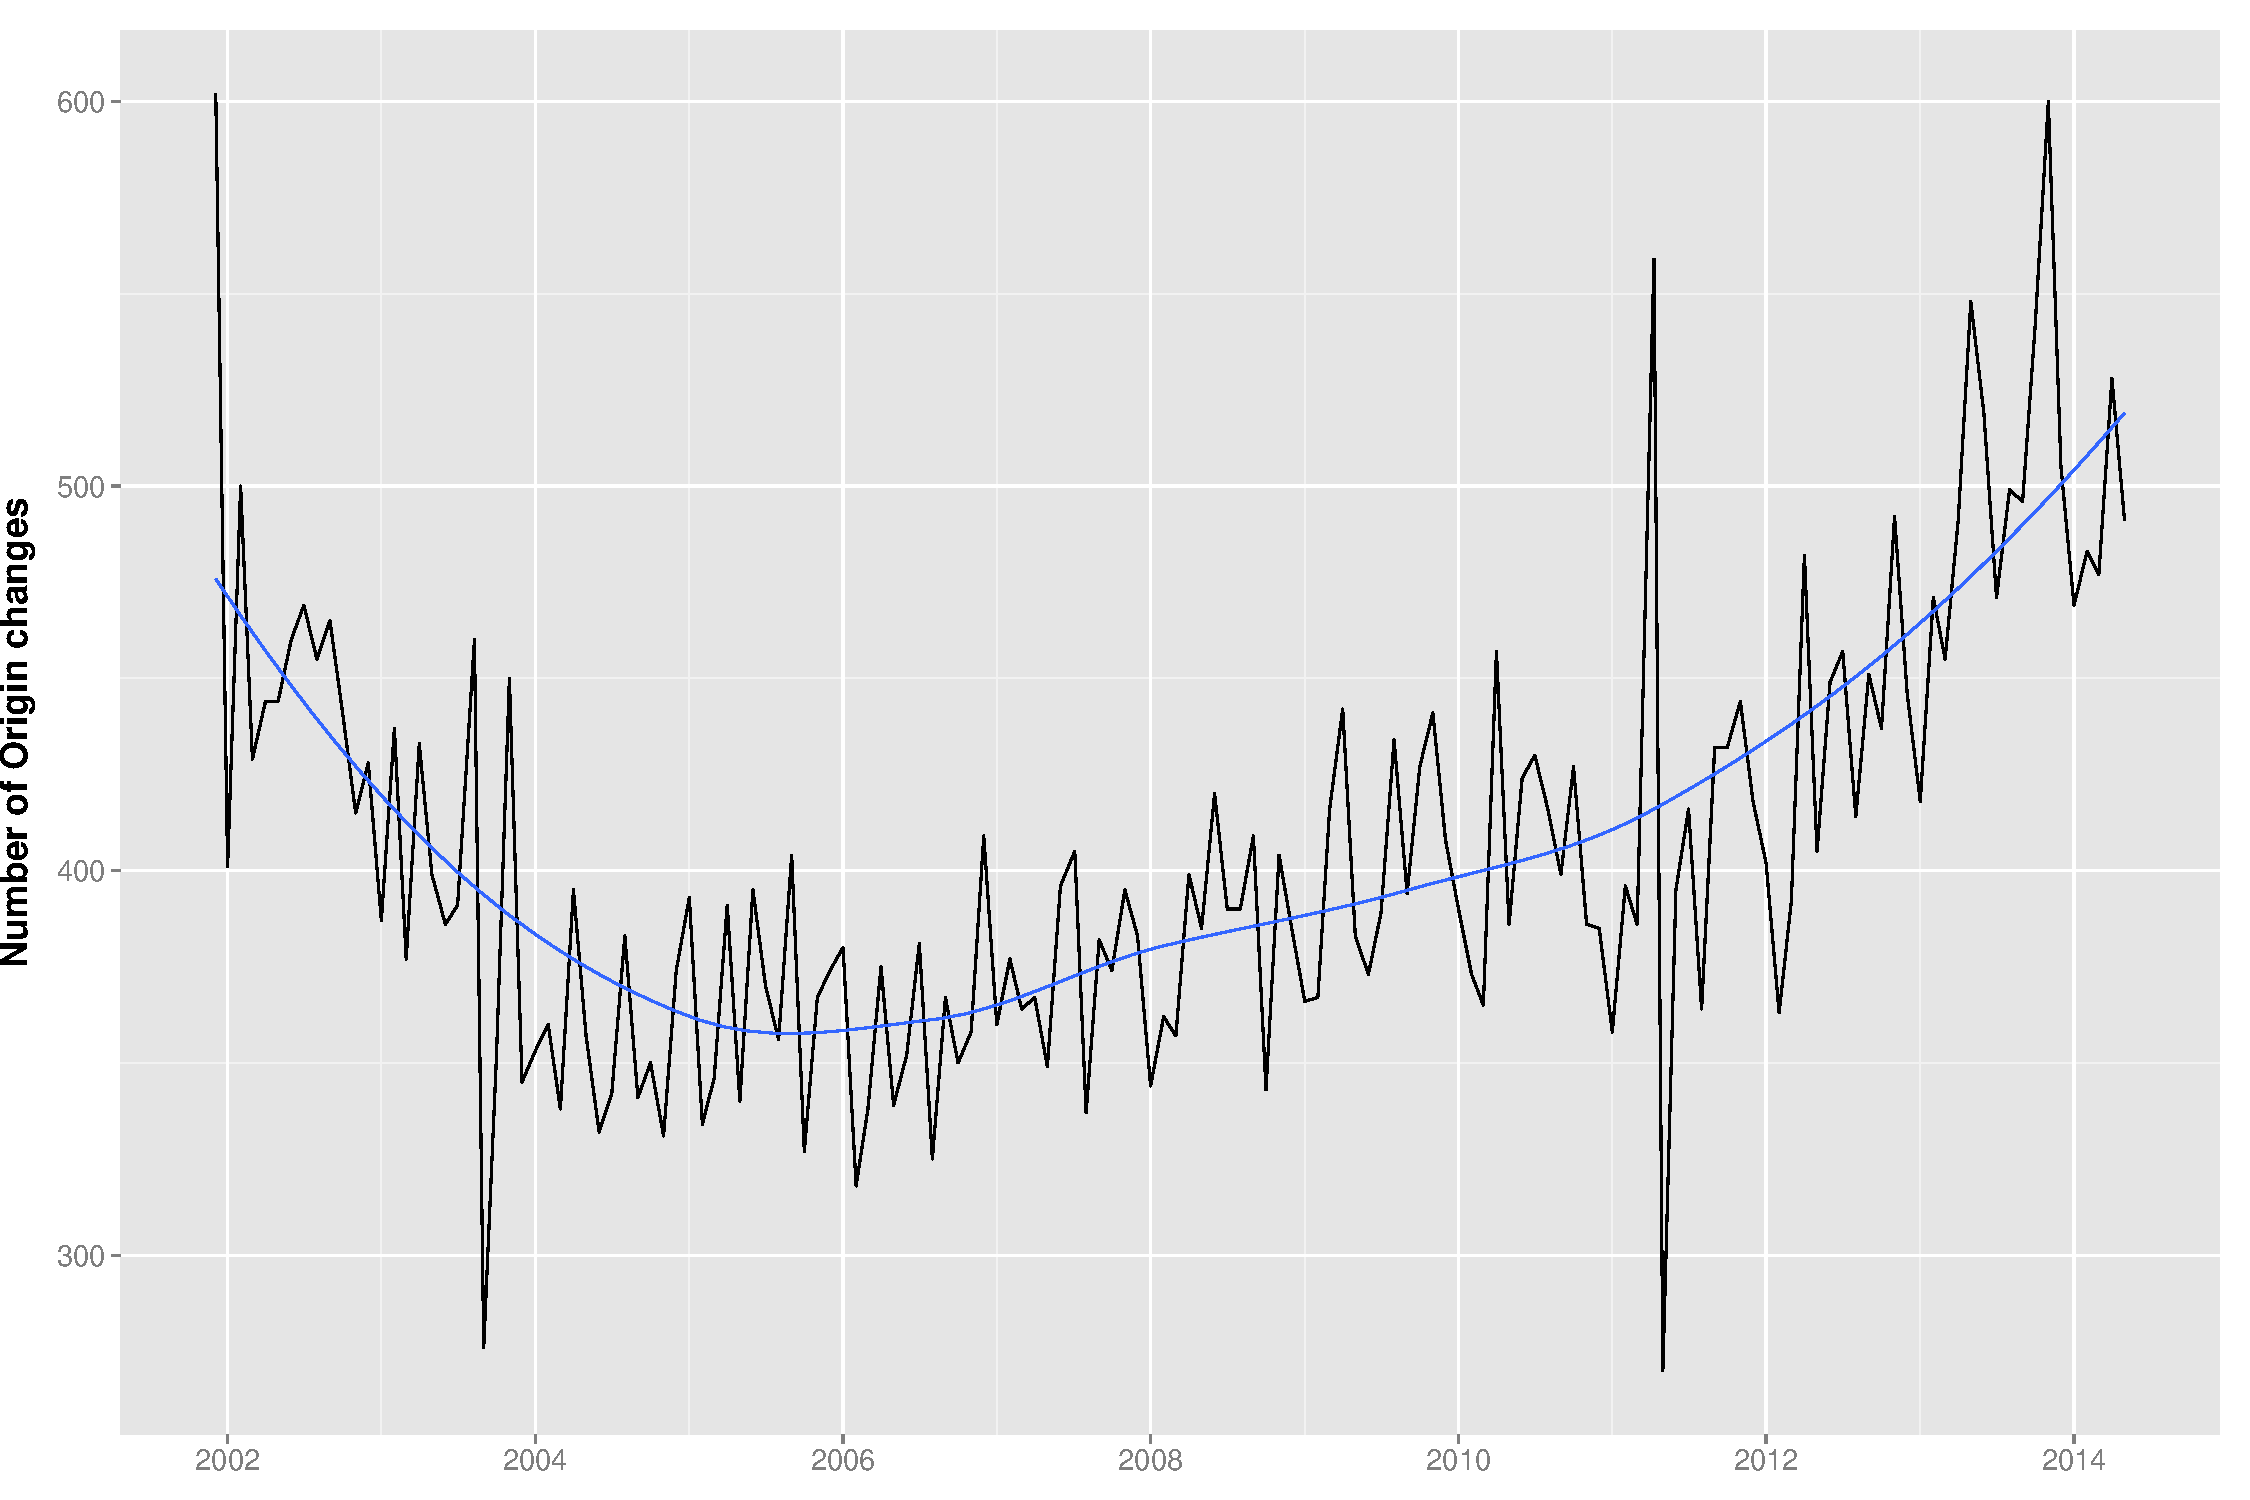
\includegraphics[scale=0.35]{compareAggregation.pdf}
\caption{Observed number of monthly
unique origin-origin pair changes, after aggregating equal origin-origin pairs}
\label{fig:compareAggregation}
\end{figure}







We can see that some of the peaks dissapeared and that the graph progression turned a bit "smoother" in comparison with Figure \ref{fig:comparePrefixes}. This means that many of the origins changes that occurred were between the same pair of ASes. We also continue to notice along the time period a growing trend in the number of origin changes.
In Figure \ref{fig:compareAggregation24} we applied the same principle, but now after decomposing the advertised prefixes into /24 subnets. 


\begin{figure}[!h]
\centering
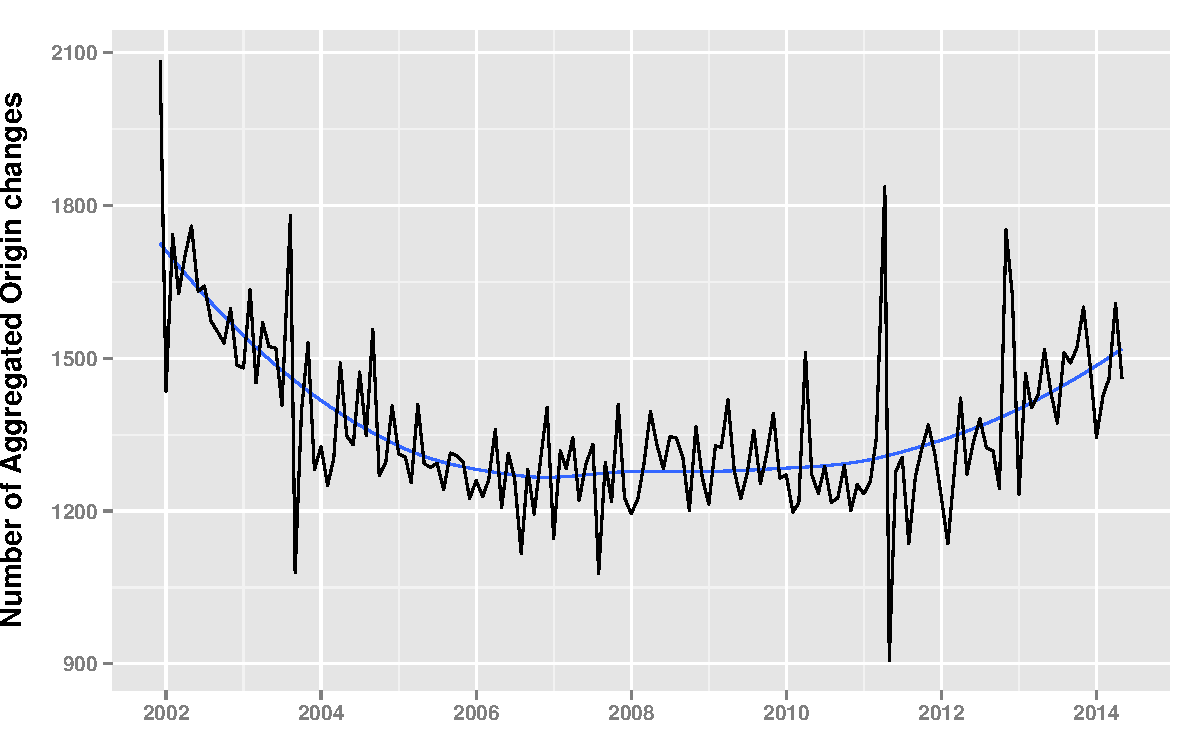
\includegraphics[scale=0.35]{compareAggregation_24.pdf}
\caption{Observed number of monthly
unique origin-origin pair changes, after aggregating equal origin-origin pairs [/24 blocks]}
\label{fig:compareAggregation24}
\end{figure}



Comparing this result with Figure \ref{fig:comparePrefixes_24} we can see huge differences. We can also notice that the graph progression became "smoother". By decomposing the advertised prefixes into /24s subnets we will get some extra information. In the previous Figure \ref{fig:compareAggregation} we were just considering exact matches between advertised prefixes from one iteration to the next. For example, if the two prefixes 1.1.0.0/16 and 1.1.1.0/24 are being advertised by AS1 and AS2 respectively and 1.1.0.0/16 is being advertised at a certain point in time while 1.1.1.0/24 is being advertised at the next point in time, when we test them for an exact match, they will not match, but if instead we decompose them into /24s, they will match for the 1.1.1.0/24 subnet resulting in an origin change for this subnet. For this reason there are higher values in this Figure then in the previous one. Here we can have a better perception of how many origin changes in /24s are happening and also to notice some deaggregation happening.  



\begin{figure}[!h]
\centering
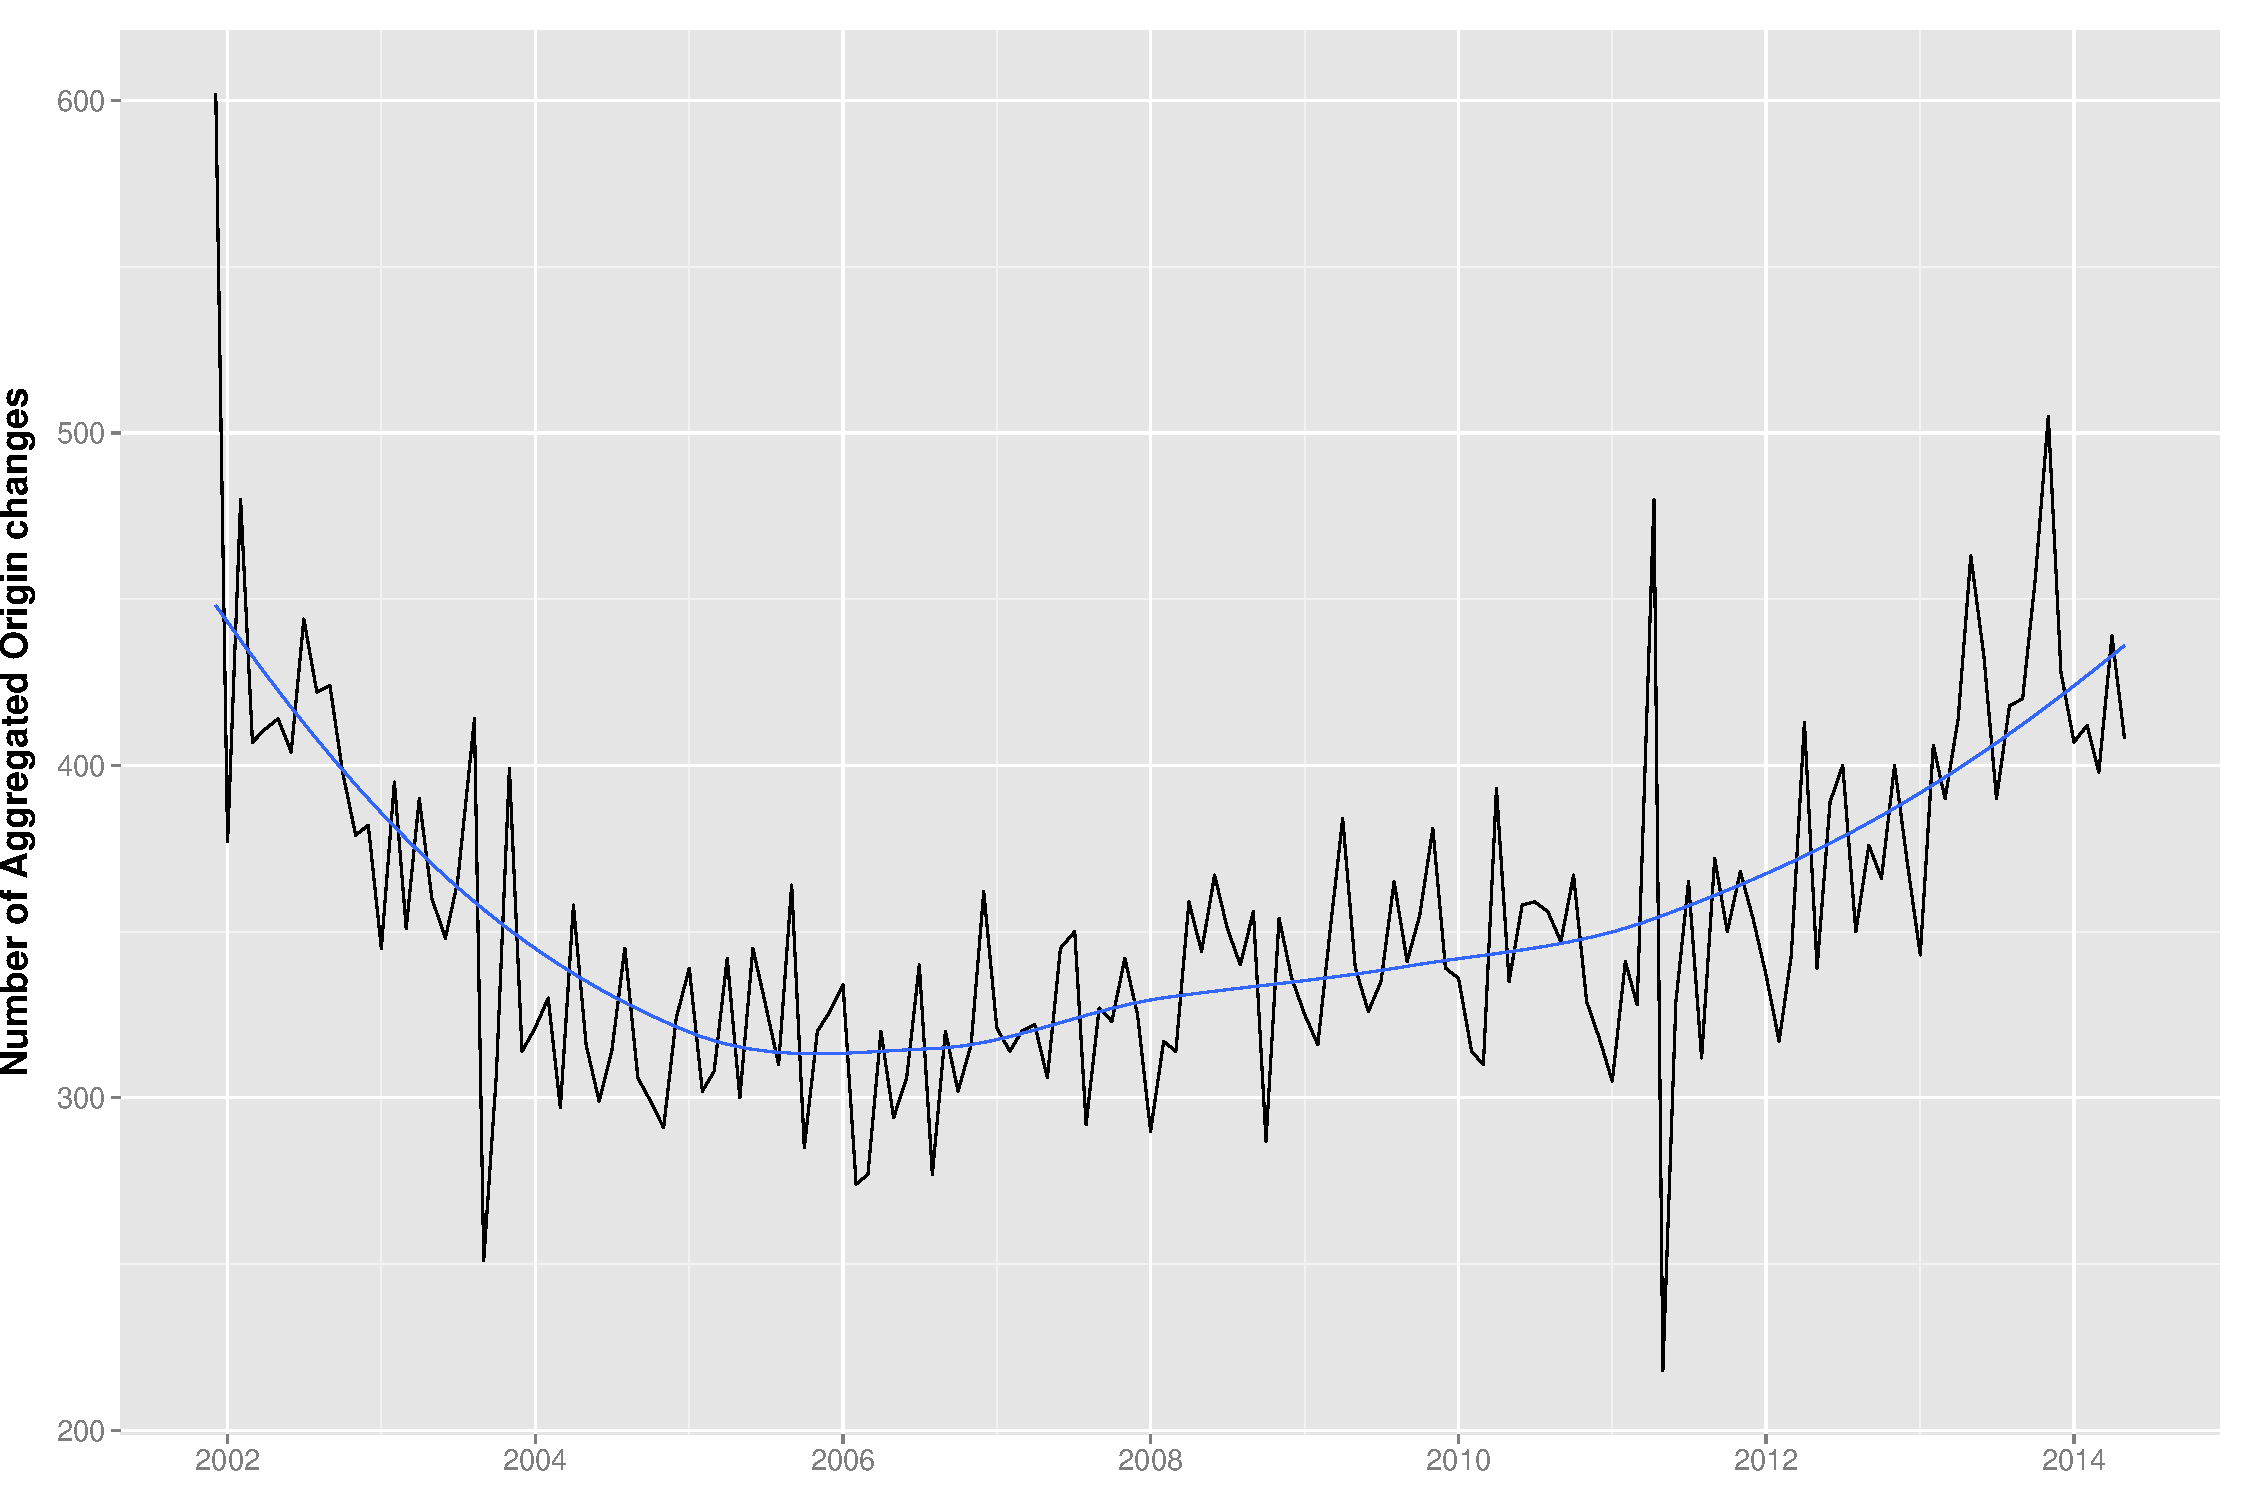
\includegraphics[scale=0.35]{compareAggregationCycles.pdf}
\caption{Observed number of monthly
unique origin-origin pair changes, after origin-origin pair aggregation and origin-origin cycles}
\label{fig:compareAggregationCycles}
\end{figure}

In Figure \ref{fig:compareAggregationCycles} the procedure was basically the same, but here we also took into consideration the situation where the prefix origin changes to a different one and then at a certain point in time returns to the previous one, making somewhat of a cycle in its evolution. Considering the prefix 1.1.0.0/16 being advertised by AS1 in a certain point in time. In the next time period it changes its origin AS to AS2 and starts to be counted as an origin change. If at a later point in time this prefix starts to be advertised again by AS1 we remove it from the counting as a change. Here we remove situations where institutions that have more than one AS number, use them for traffic engineering, for example.  In comparison with Figure \ref{fig:compareAggregation} we can see that the graph progression became "smoother" and that the overall value of prefix changes got lower.

\begin{figure}[!h]
\centering
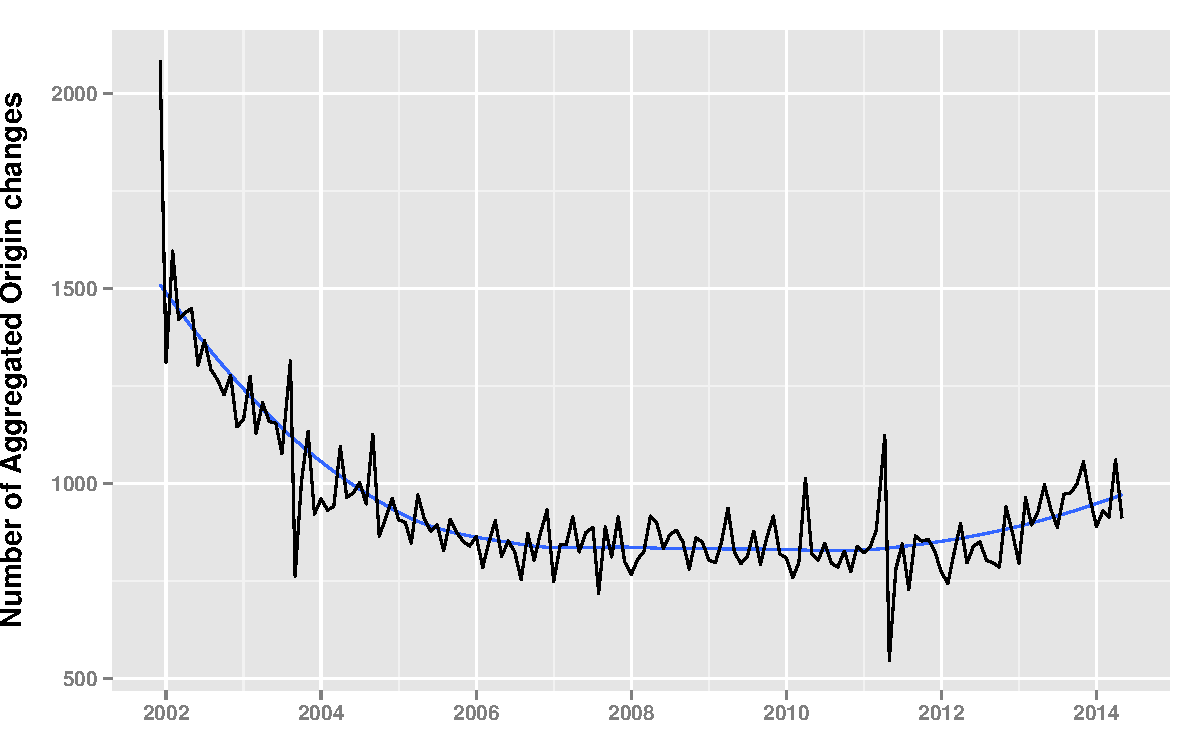
\includegraphics[scale=0.35]{compareAggregationCycles_24.pdf}
\caption{Observed number of monthly
unique origin-origin pair changes, after origin-origin pair aggregation and origin-origin cycles [/24 blocks]}
\label{fig:compareAggregationCycles24}
\end{figure}

Figure \ref{fig:compareAggregationCycles24} shows the results of applying this cycle removal to Figure \ref{fig:compareAggregation24}. We can again see that the graph progression became "smoother" and that the overall value of prefix changes got lower. 

\section{Address Allocation}

Our next analysis inferred on the number of days that passed sinced a prefix was allocated and started to be routed. Here we take the prefixes allocated from the allocation files and deaggregate them into /24 subnets. We then use these subnets to search in BGP raw data a first time that we see an occurrence of the subnet and when we encounter one we calculate the days that passed since it was allocated. We use a allocation filter so that when we search through the BGP raw data we only do a positive match if the encountered prefix has already been before the time instance of the BGP file.  

\begin{figure}[!h]
\centering
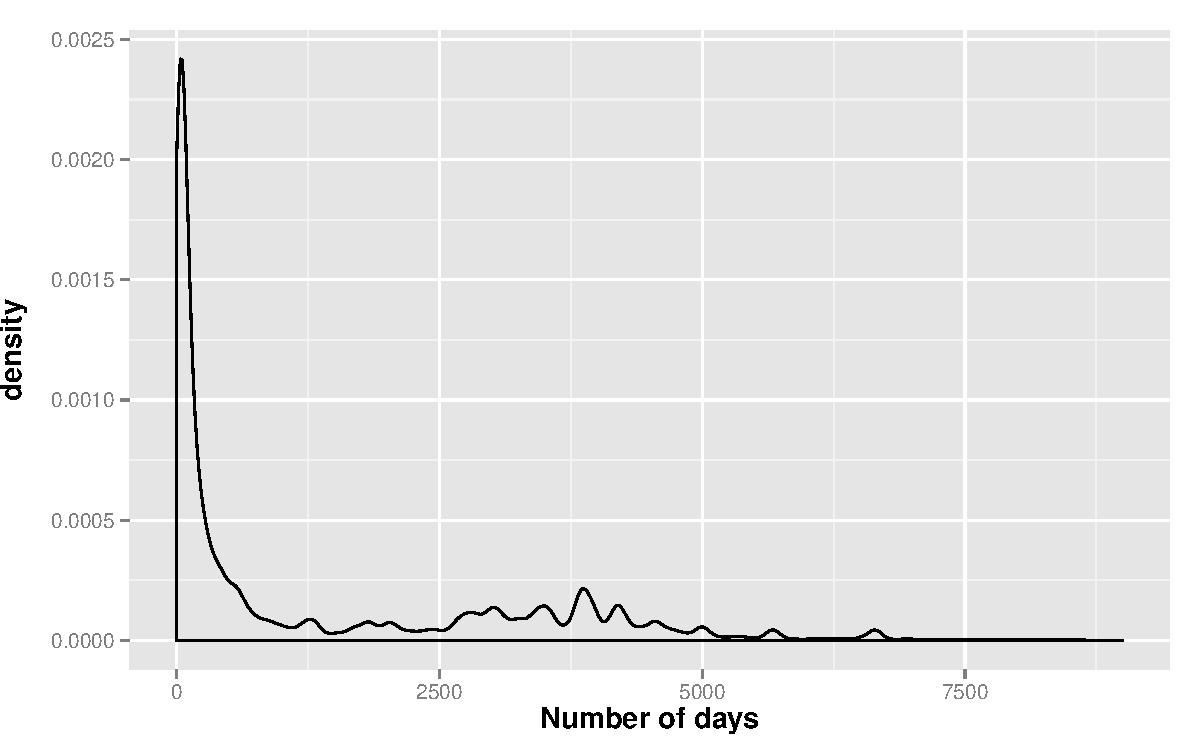
\includegraphics[scale=0.35]{densityGlobal.pdf}
\caption{Density plot of days that passed since prefixes are allocated until they are advertised in BGP}
\label{fig:densityGlobal}
\end{figure}

In Figure \ref{fig:densityGlobal} it is shown a density plot regarding the number of days that passed. We can see that the higher density is until 1250 days that passed. We can then see that the density increased again between 2500 and 5000 days. This is due to the fact that the allocation files contain allocations since 1982 while there are only BGP data files since 2001. For this reason we decided to just process allocations made after the year 2001, or our results would be biased. Just by analyzing the plot it is hard to get to a conclusion and some statistical values are important, such as maximum = 11315, mean = 1327.47, median = 256 and standard deviation = 1763.316. 
Has we can see in Figure \ref{fig:densityGlobal2001}, the density values that were shown between 2500
and 5000 days  are not present anymore and the density values are now between 0 and 1000, being the majority between 0 and 250. If we compare the previous statistical values with the current ones,maximum = 4338, mean = 155.1632, median = 56 and standard deviation = 246.6986, we can notice a huge difference. The maximum value is almost three times less, the mean eight times less,the median around five times and the standard deviation also much lower. This was due to be considering allocated prefixes before 2001 and the sample was being biased.

\begin{figure}[!h]
\centering
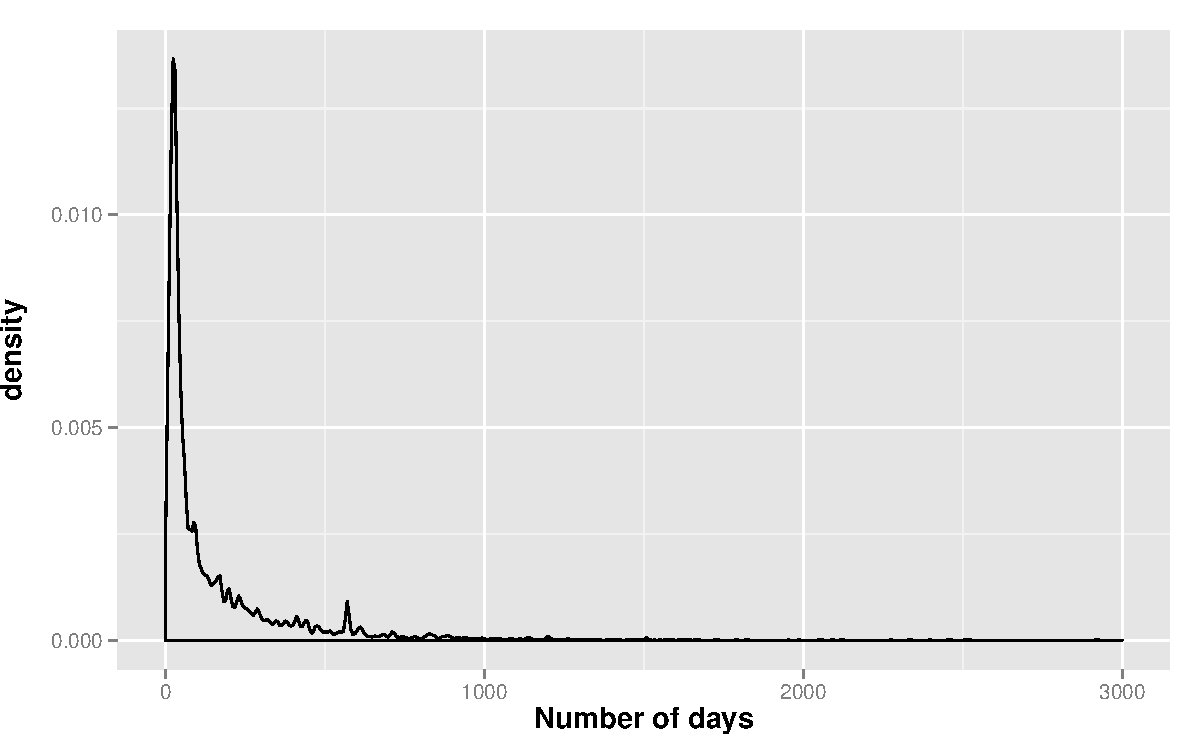
\includegraphics[scale=0.35]{densityGlobal2001.pdf}
\caption{Density plot of days that passed since prefixes are allocated, after 2001, until they are advertised in BGP}
\label{fig:densityGlobal2001}
\end{figure}

An important day for our analysis is February 3 2011, when the Internet Assigned Numbers Authority allocated the remaining /8 blocks to the Regional Internet Registries. Therefore we decided to analyze what happen before and after this date with regards to the number of days that took for a allocated prefix to be seen in routing. Our assumption was that after 2011 and after the RIRs changed their allocation polices, companies needing IPv4 addresses would also use them faster then before. 
The results for before February 3, 2011 are shown in Figure \ref{fig:densityBefore2001}. Once again we have to limit our study to prefixes allocated after 2001.  


\begin{figure}[!h]
\centering
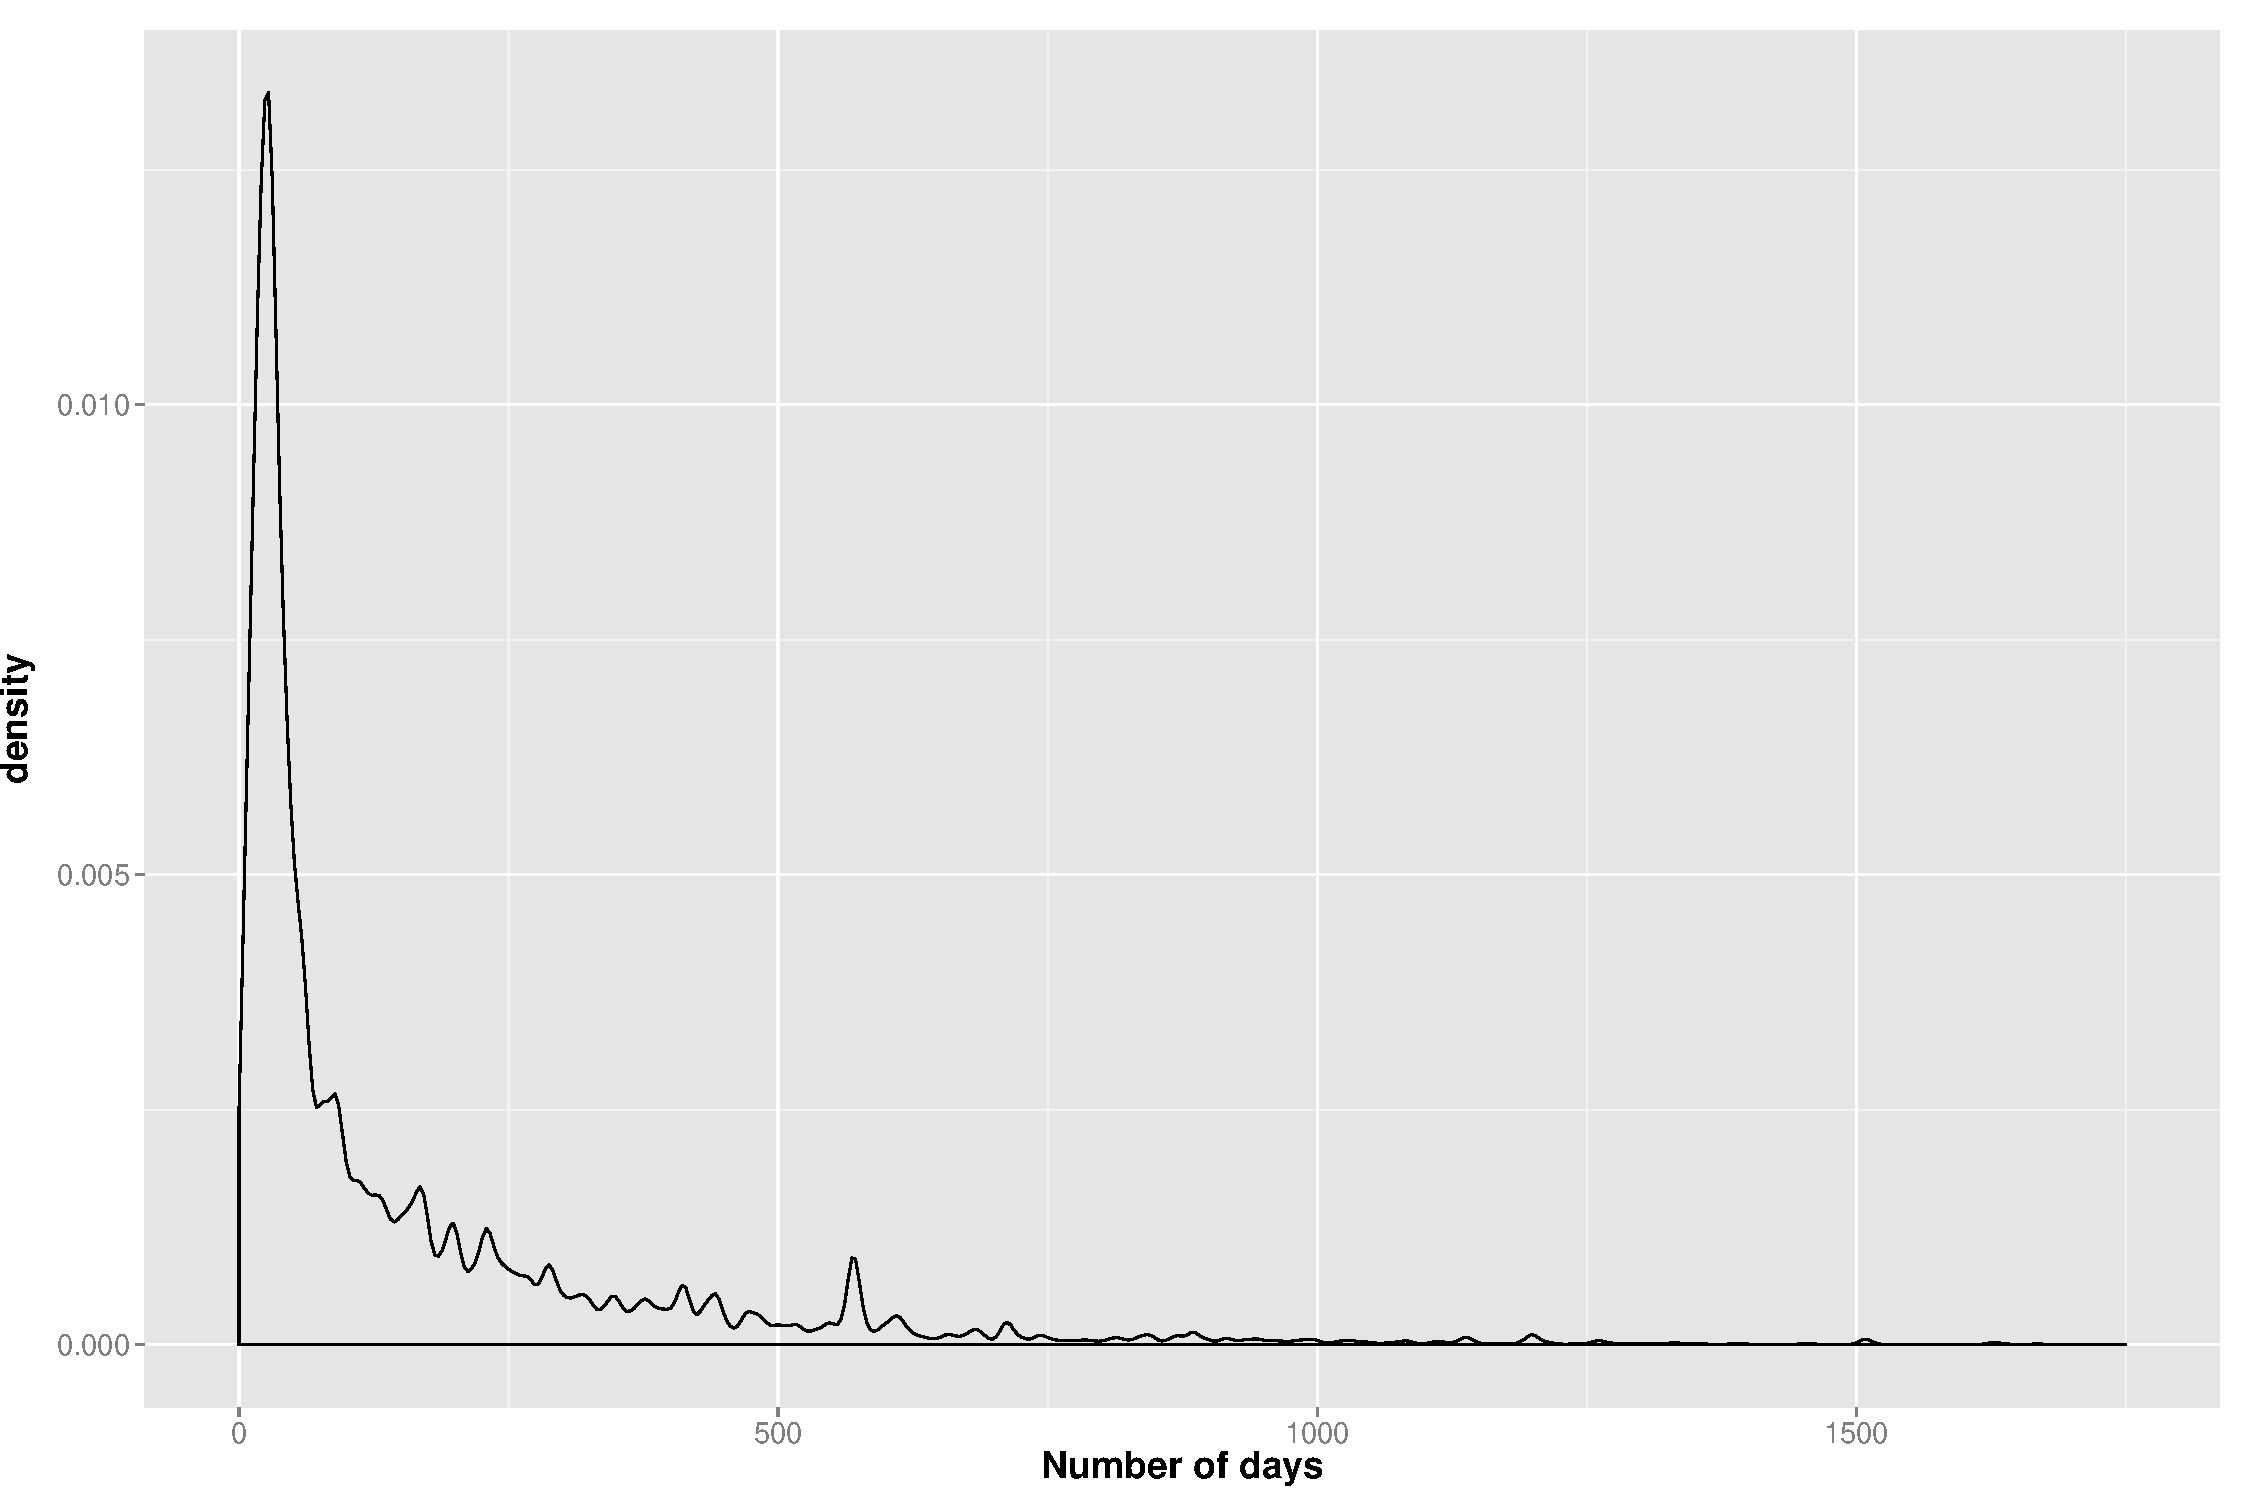
\includegraphics[scale=0.35]{densityBefore2011.pdf}
\caption{Density plot of days that passed since prefixes are allocated, between 2001 and 2011, until they are advertised in BGP}
\label{fig:densityBefore2001}
\end{figure}

The statistical values for this distribution are: maximum = 4338; mean = 162.2353; median = 58 and standard deviation = 255.6121. We can already see that the maximum value for this distribution is the same as the value for the global distribution and the mean was higher then the global one. This is already an indication that this distribution has some of the biggest values in term of days passed. When we consider the median and the standard deviation, we can assume that this distribution will have higher values then a distribution just considering the period after 2011, which is shown in Figure \ref{fig:densityAfter2001}.


\begin{figure}[!h]
\centering
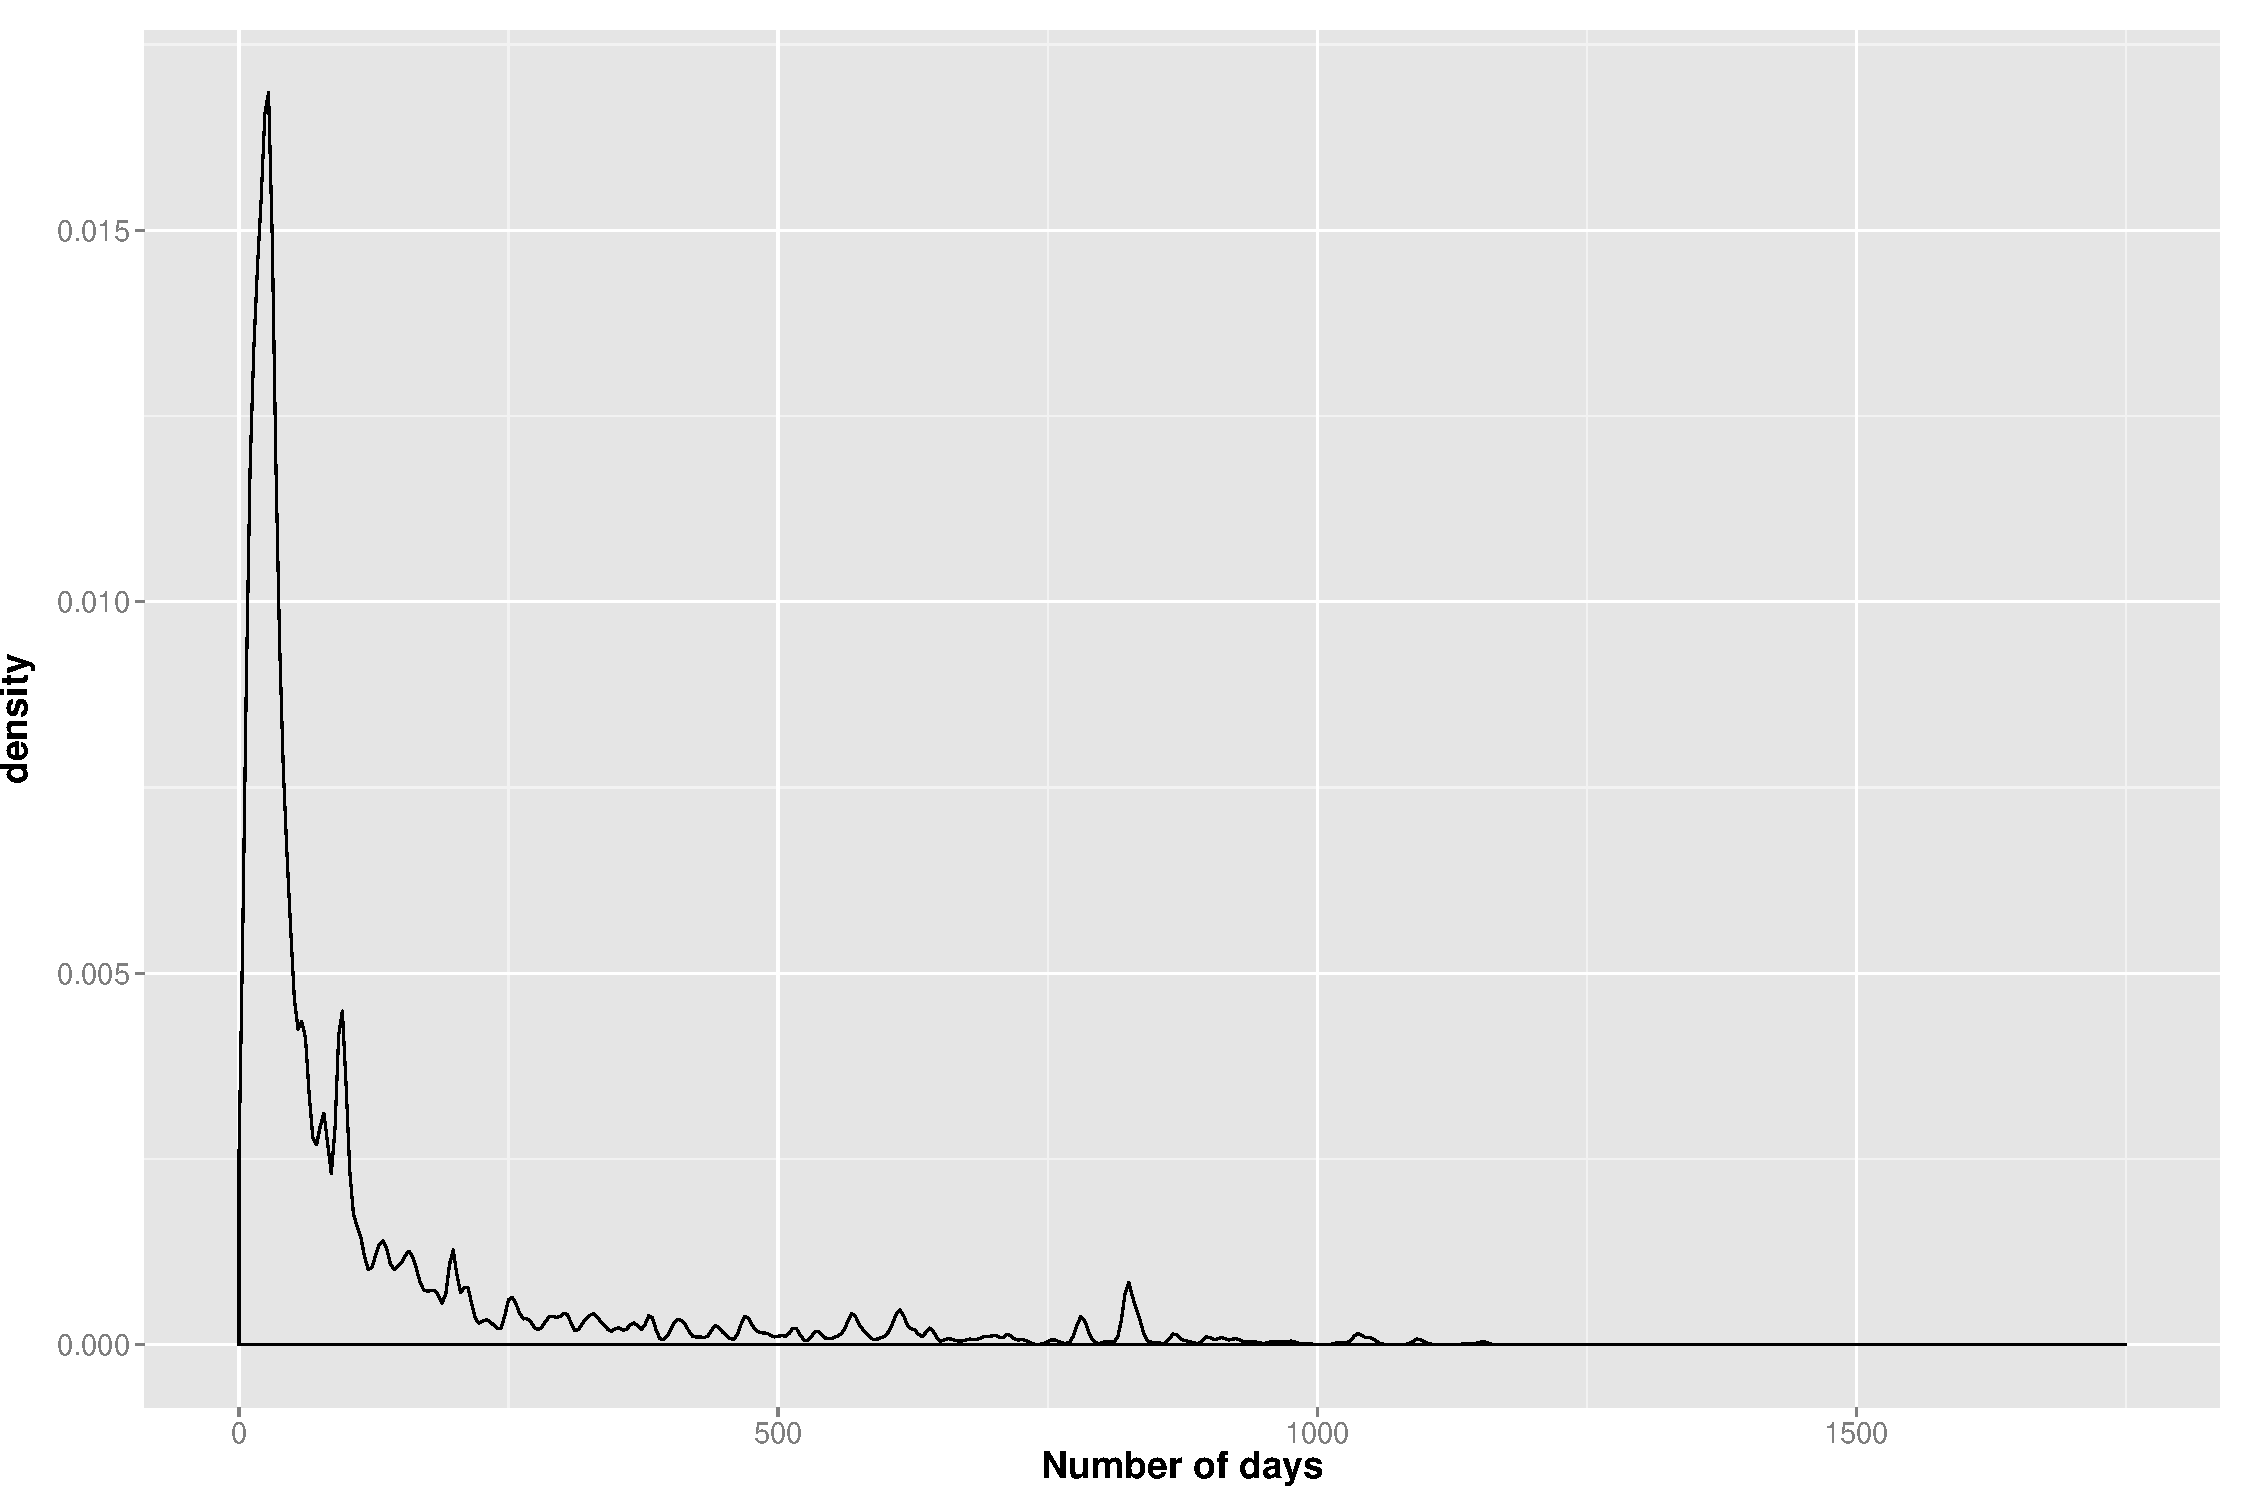
\includegraphics[scale=0.35]{densityAfter2011.pdf}
\caption{Density plot of days that passed since prefixes are allocated, after 2011, until they are advertised in BGP}
\label{fig:densityAfter2001}
\end{figure}

The statistical values for this distribution are: maximum = 1154, mean = 119.257, median = 40 and standard deviation = 191.2714. We can notice a higher density between 100 and 500 days in Figure \ref{fig:densityBefore2001} than in Figure \ref{fig:densityAfter2001}, but to reach a conclusion we need to compare the statistical values. By comparing them we can see that the distribution from before 2011 has a higher maximum value, higher mean, higher median and a higher standard deviation. We can conclude that the prefixes allocated after 2011 take in average less time to be seen in the BGP raw data than the ones allocated before. We need to make a reamark and refer that the time span between 2001 and 2011 is bigger than from 2011 and 2014. This means that we can have prefixes that were allocated between 2011 and 2014 and they were still not seen in the BGP data, being possible to seem them at a later point in time, changing the values that were see now.

\begin{figure}[!h]
\centering
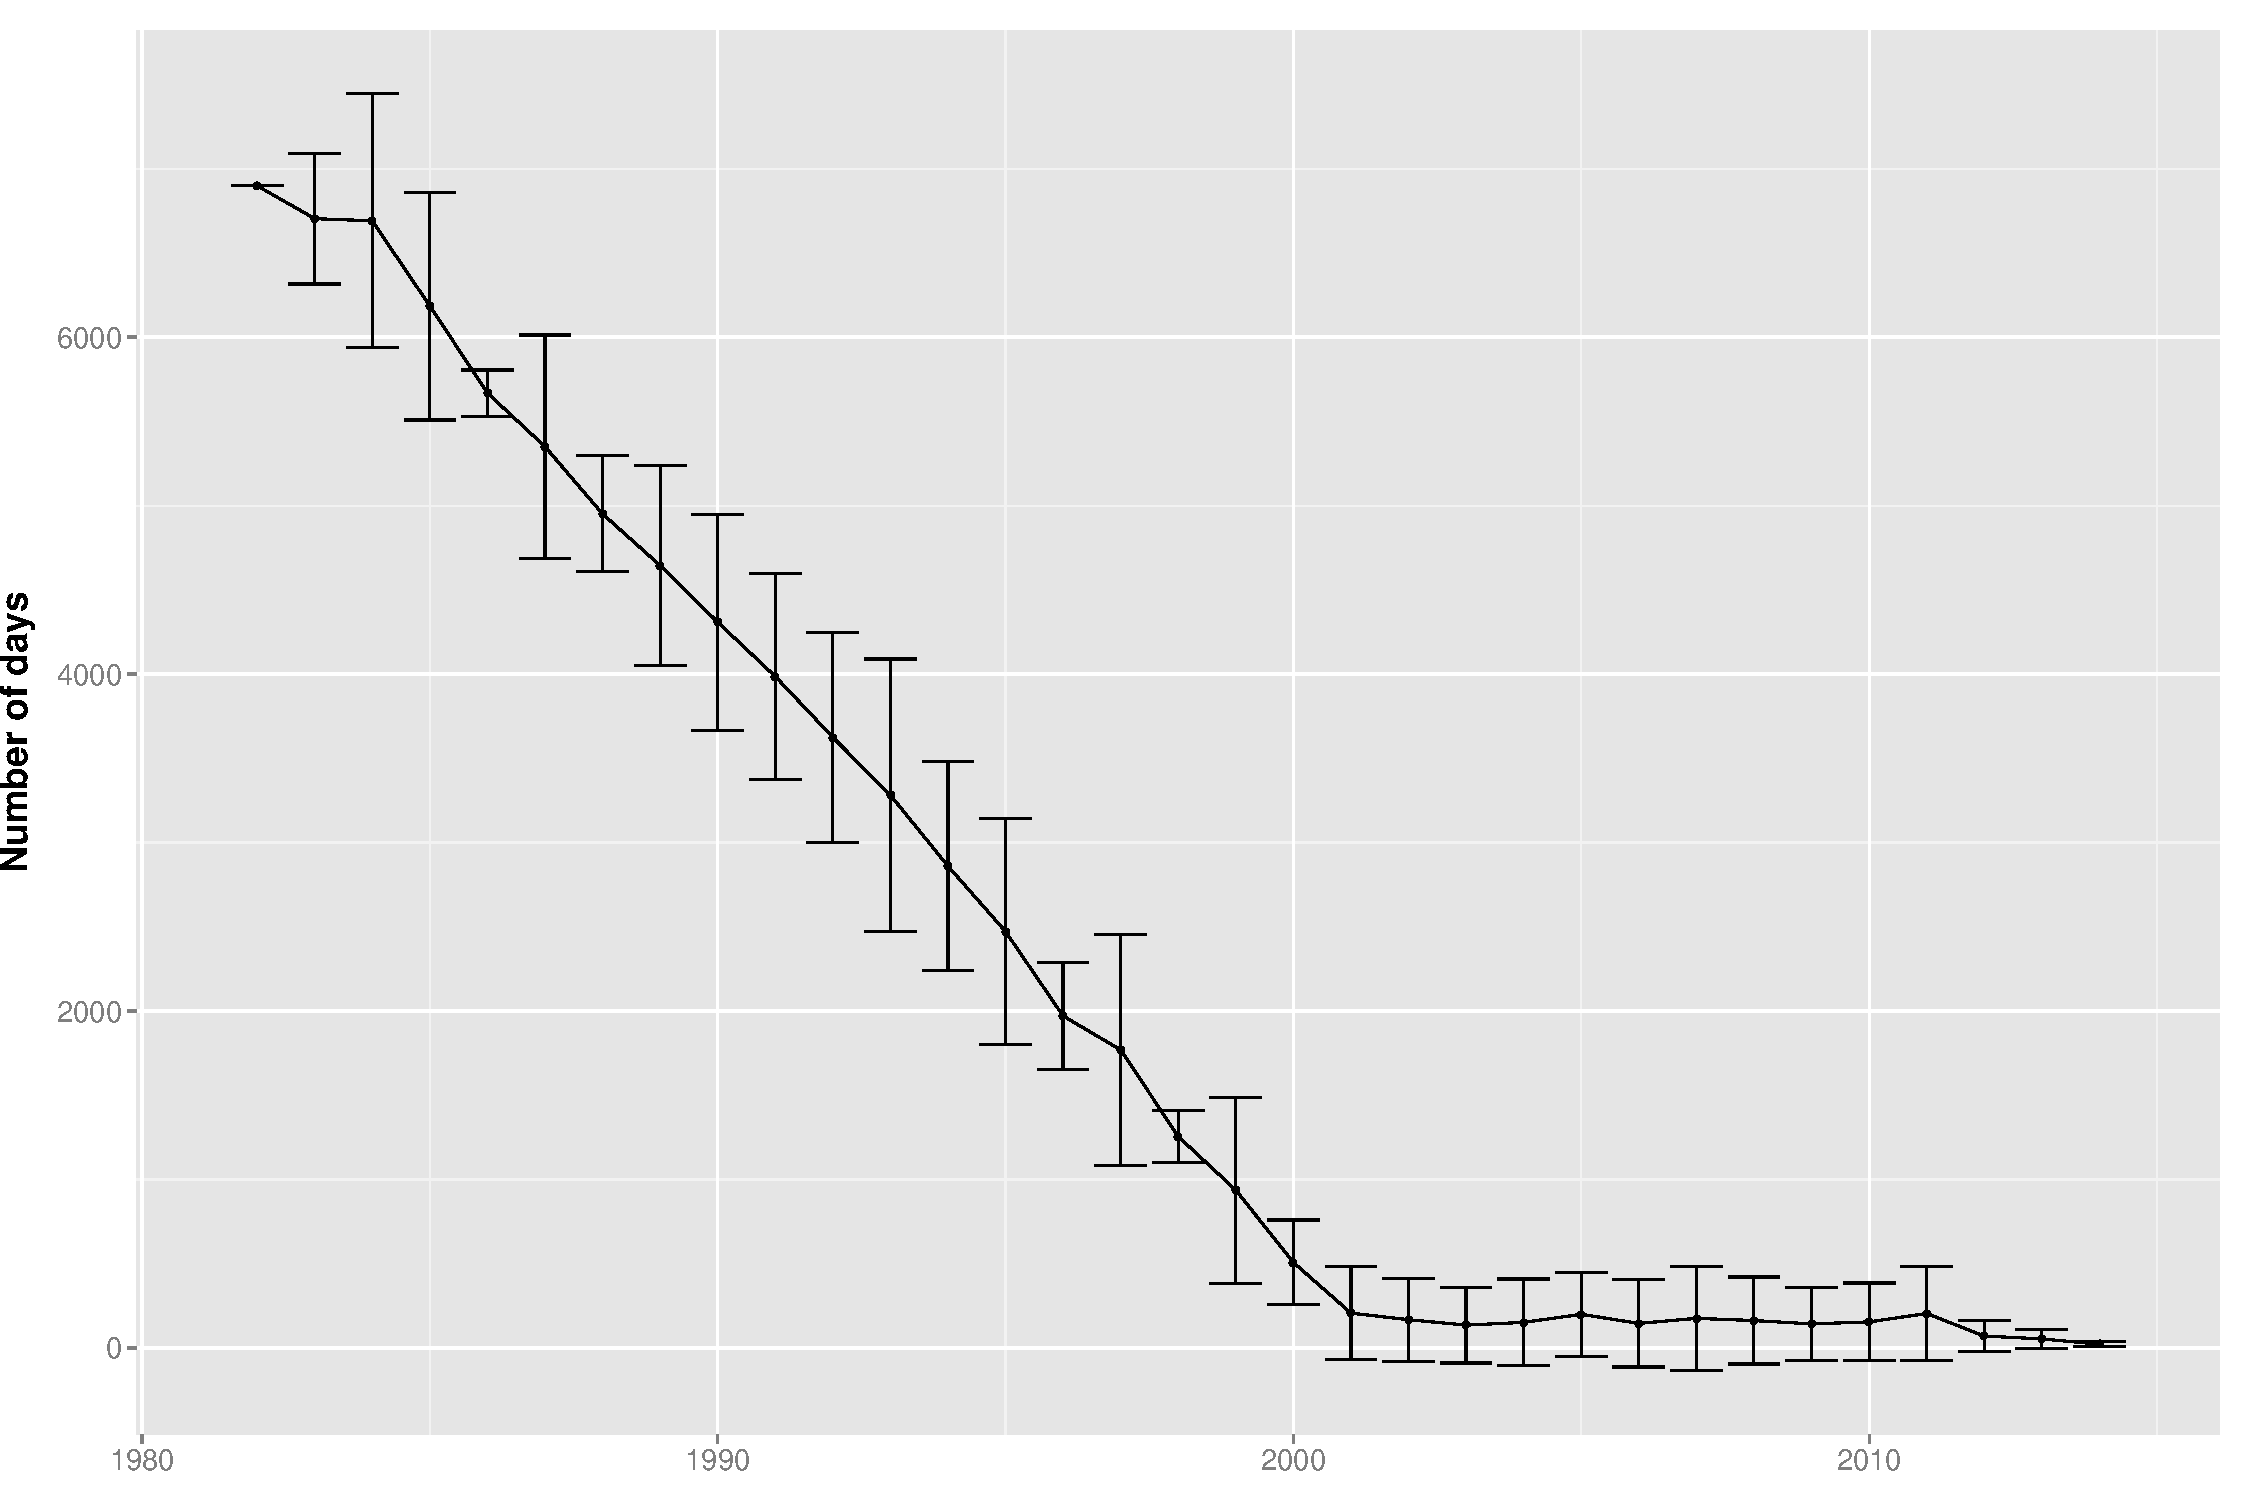
\includegraphics[scale=0.35]{densityYearly.pdf}
\caption{Observed average number of days that passed since prefixes are allocated until they are advertised in BGP along the years}
\label{fig:densityYearly}
\end{figure}

In Figure \ref{fig:densityYearly} is represented the average number of days that passed for the prefixe to be seen in routing for each year of allocation. We can see that since 1982 until 2001 the values are decreasing linearly, due to the issue stated before. In  Figure \ref{fig:densityYearlyShort} is represented the relevant time period from 2001 until 2014. It is possible to see that the values were relatively constant until 2011 and since then they started to decrease. Again it can mean that since then prefix holders are using the prefixes quickly, but to be absolutely sure we needed a higher time span.


\begin{figure}[!h]
\centering
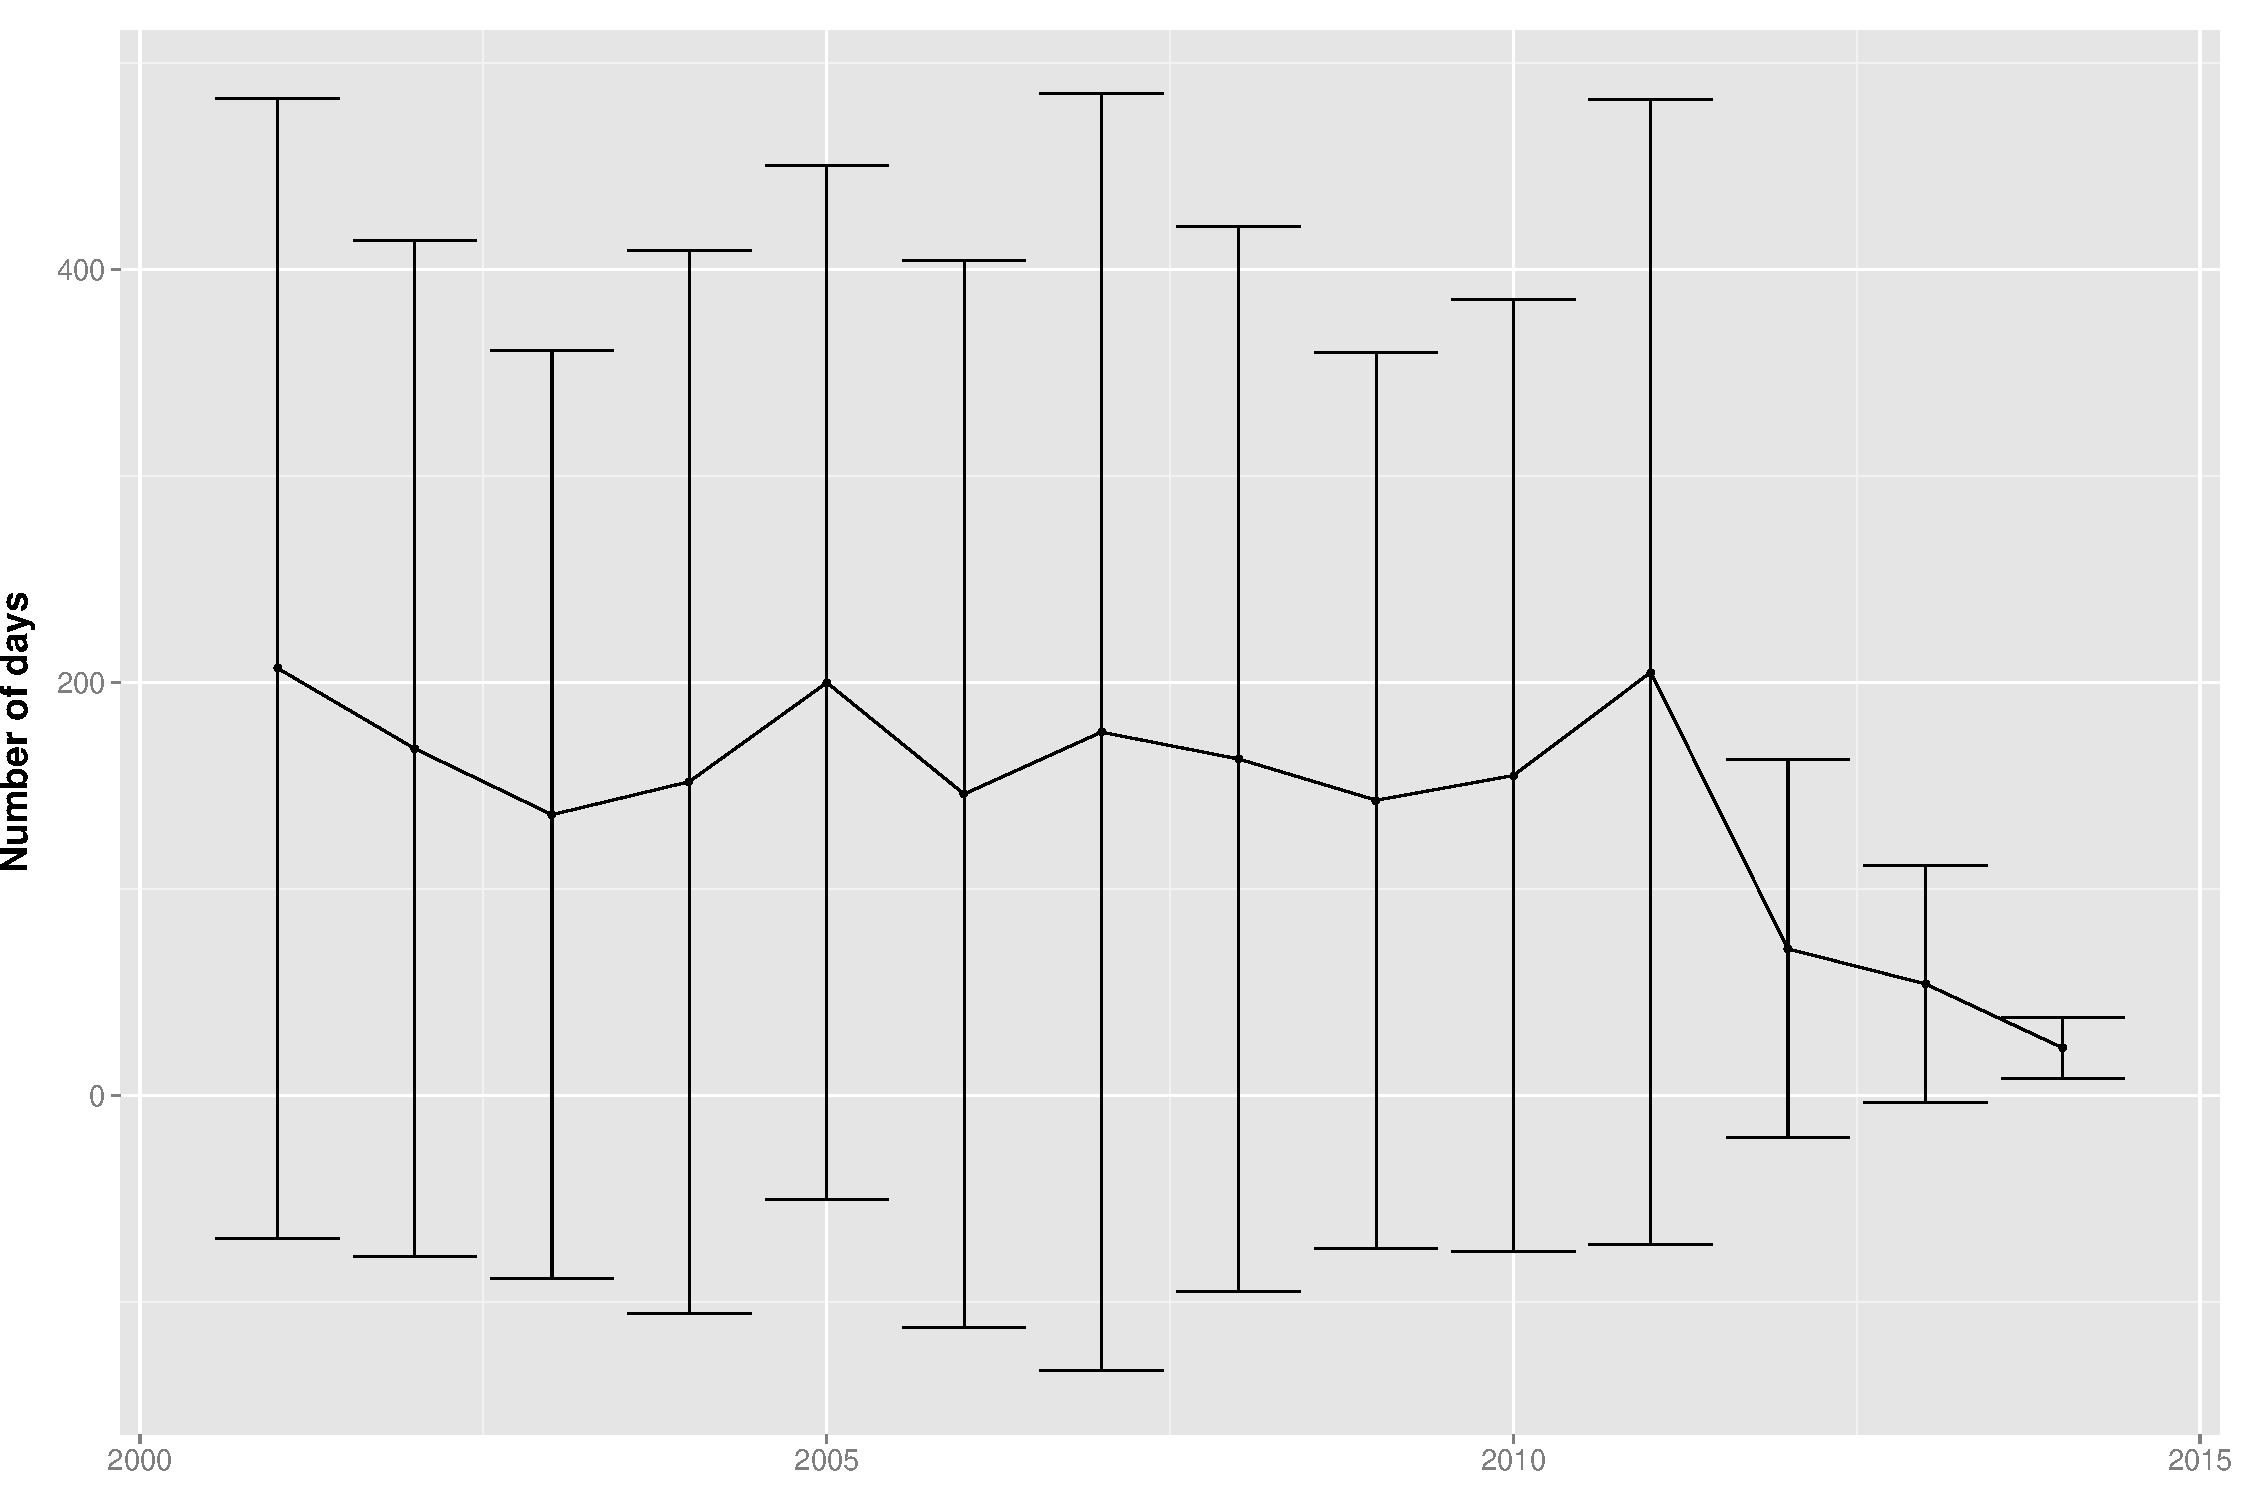
\includegraphics[scale=0.35]{densityYearlyShort.pdf}
\caption{Observed average number of days that passed since prefixes are allocated until they are advertised in BGP, after 2001}
\label{fig:densityYearlyShort}
\end{figure}

\section{BGP Routing Dynamics}

\subsection{Routing Status}
The next step in our work was to analyze the routing dynamics, in particular to see the amount of prefixes that are being advertised in BGP and its behaviour. 
In Figure \ref{fig:routingStatusGlobal} it is shown the number of allocated prefixes and their routing status. We define routing status as: full routed prefixes; partially routed prefixes and not routed prefixes. Full routed prefixes are the considered to be prefixes that have their entire address space being advertised, partially routed prefixes are the ones that have at least a part of their address space being advertised, but not the entire one and not routed prefixes are the ones that don't have any part of their address space being advertised. The total number of prefixes is the number of prefixes that were allocated until that point in time.

\begin{figure}[!h]
\centering
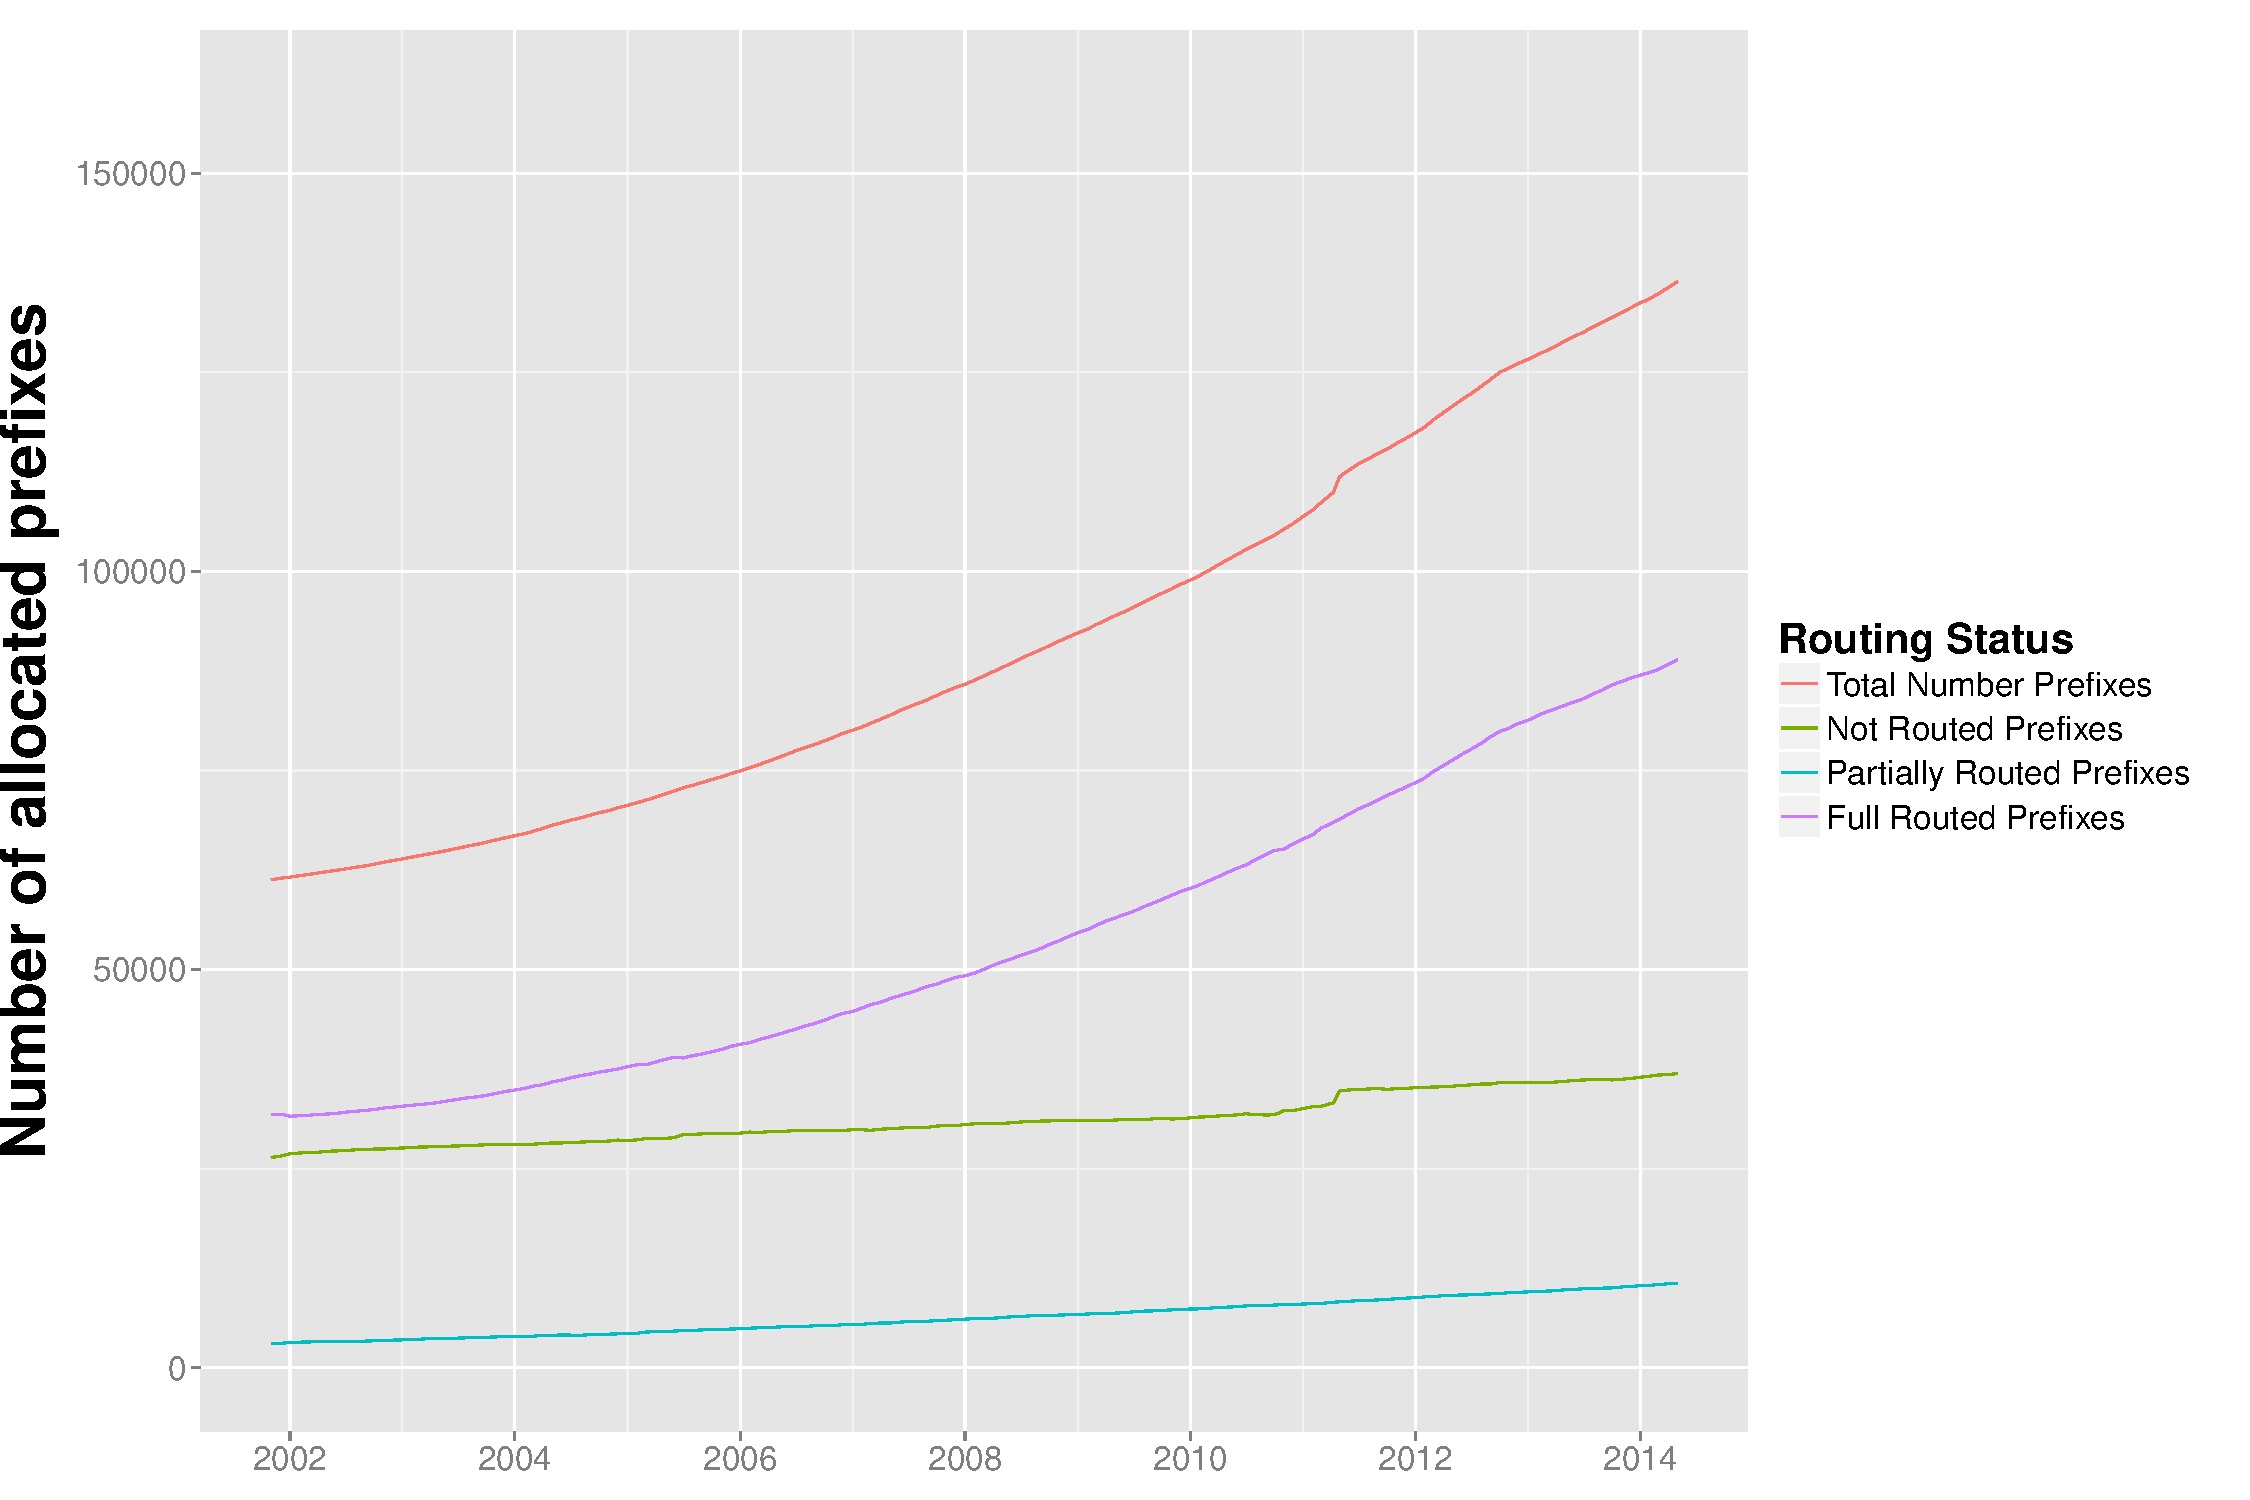
\includegraphics[scale=0.35]{routeStatusGlobal.pdf}
\caption{Number of allocated prefixes that are being advertised in BGP and their routing status}
\label{fig:routingStatusGlobal}
\end{figure}

As expected we can see that the number of allocated prefixes has been increasing quite fast and the number of full routed prefixes has followed the same trend. The number of not routed prefixes and partially routed prefixes also increase but at a very slow rate when compared to the full routed prefixes. It was expected to see this type of trend, because as the number of allocated prefixes increase it is expected that all the other routing status increase and as expected the full routed increase at a much higher rate. What was a surprise was the fact that since the start of our time period there where so many not routed prefixes, which could be due to old allocations.

\begin{figure}[!h]
\centering
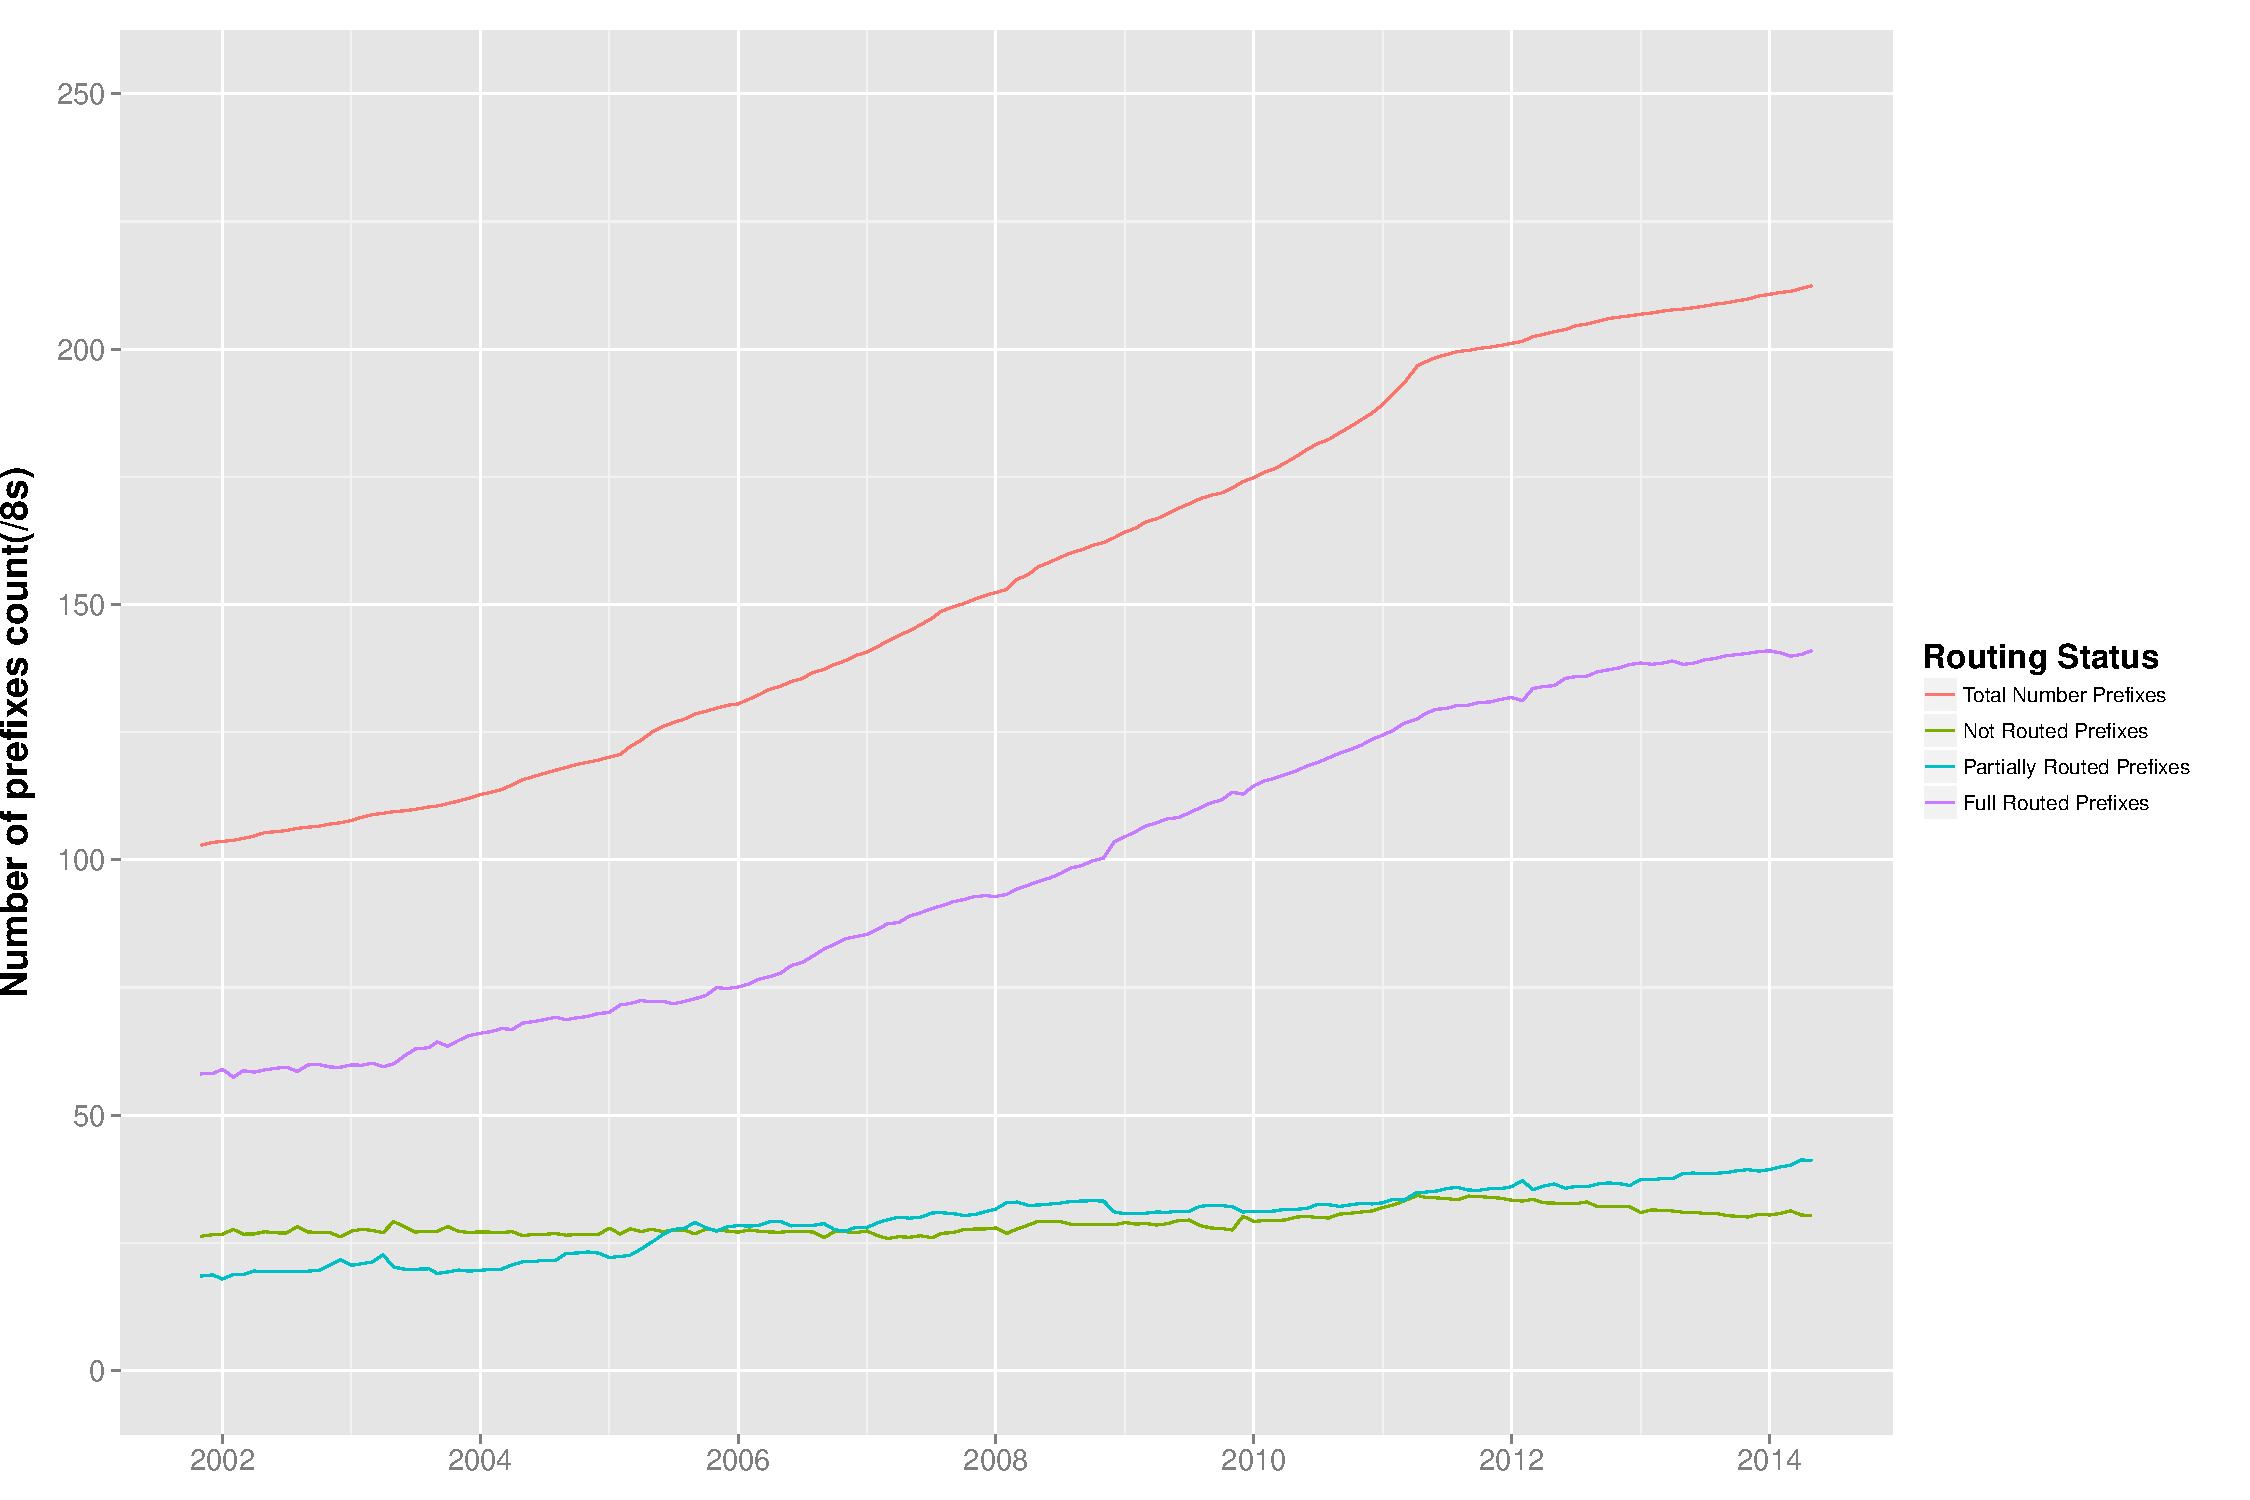
\includegraphics[scale=0.35]{routeStatusGlobal8.pdf}
\caption{Amount of address space of allocated prefixes that is being advertised in BGP in /8s, according to prefixes routing status}
\label{fig:routingStatusGlobal8}
\end{figure}

In Figure \ref{fig:routingStatusGlobal8} we can see the same distribution, but these time showing the number of prefixes count in /8s, so that we are able to quantify the address space that we are dealing with. We can see that the number of total prefixes and full routed ones follow the same trend, increasing at a fast pace. For a value of around 212 /8s of allocated prefixes there are around 140 /8s being fully routed. Regarding the number of partially routed prefixes and not routed prefixes we can see a change in comparison with the previous Figure, where the number of not routed prefixes was three times higher that the number of partially routed ones. Even more in Figure \ref{fig:routingStatusGlobal8} the number of partilly routed prefixes /8s overcome the number of /8s that are not routed. The reason for this is that in the partially routed prefixes there are huge address blocks that are not completely routed where for the not routed routed there are many smaller blocks of addresses.  

\begin{figure}[!h]
\centering
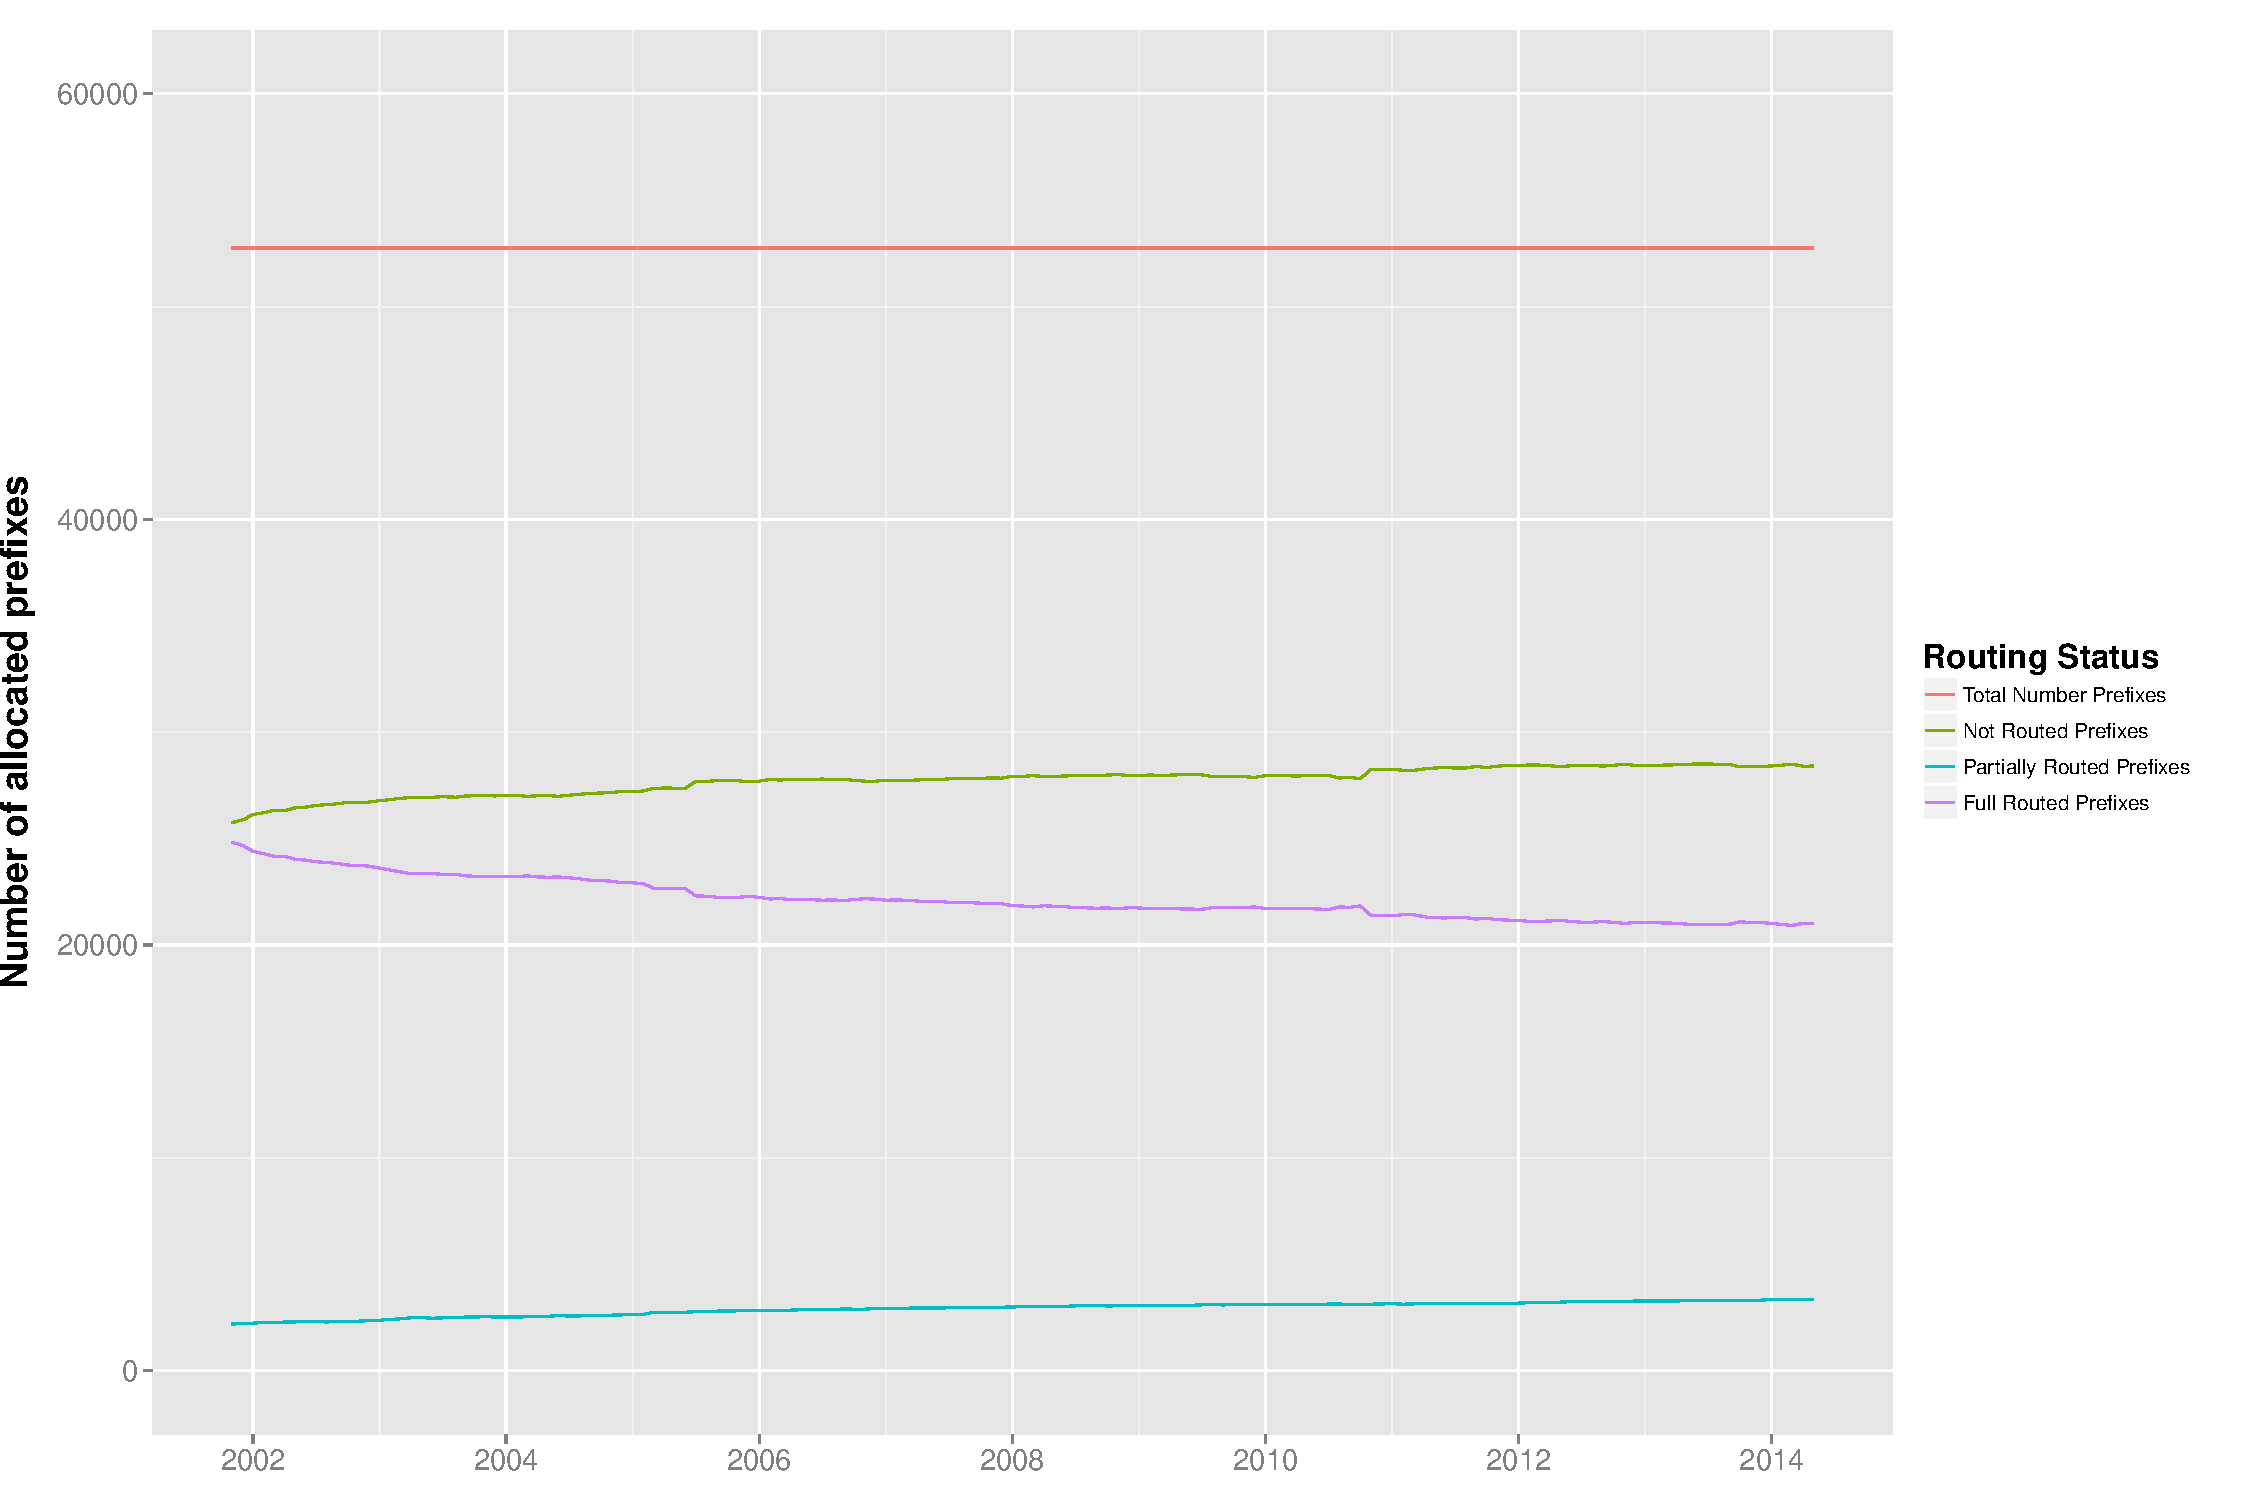
\includegraphics[scale=0.35]{routeStatusOld.pdf}
\caption{Number of allocated prefixes, allocated before 1997, that are being advertised in BGP and their routing status}
\label{fig:routingStatusOld}
\end{figure}

In order to understand the behaviour of the not routed prefixes and why since 2001 this number was already high, we divided our sample into prefixes allocated before 1997 and prefixes allocated after. This date was chosen, because it was the date when Arin was established and prefixes before this date are often considered as "legacy".
In Figure \ref{fig:routingStatusOld} we can see that for these old prefixes the value of the not routed prefixes is incredible high. With a value of 25 000 in 2001 it makes it is almost as same as the value for the global view which has a value of 26 000. By the beggining of 2014 we see that the value is 28 000 and the global view as a value of 36 000. This indicates that the majority of the not routed prefixes seen today are still from allocated blocks of addresses before 1997. We even see that the values for not routed prefixes increased slighty and the values for the full routed prefixes decreased in around the same proportion. The value for the partially routed prefixes remained pratically constant.

\begin{figure}[!h]
\centering
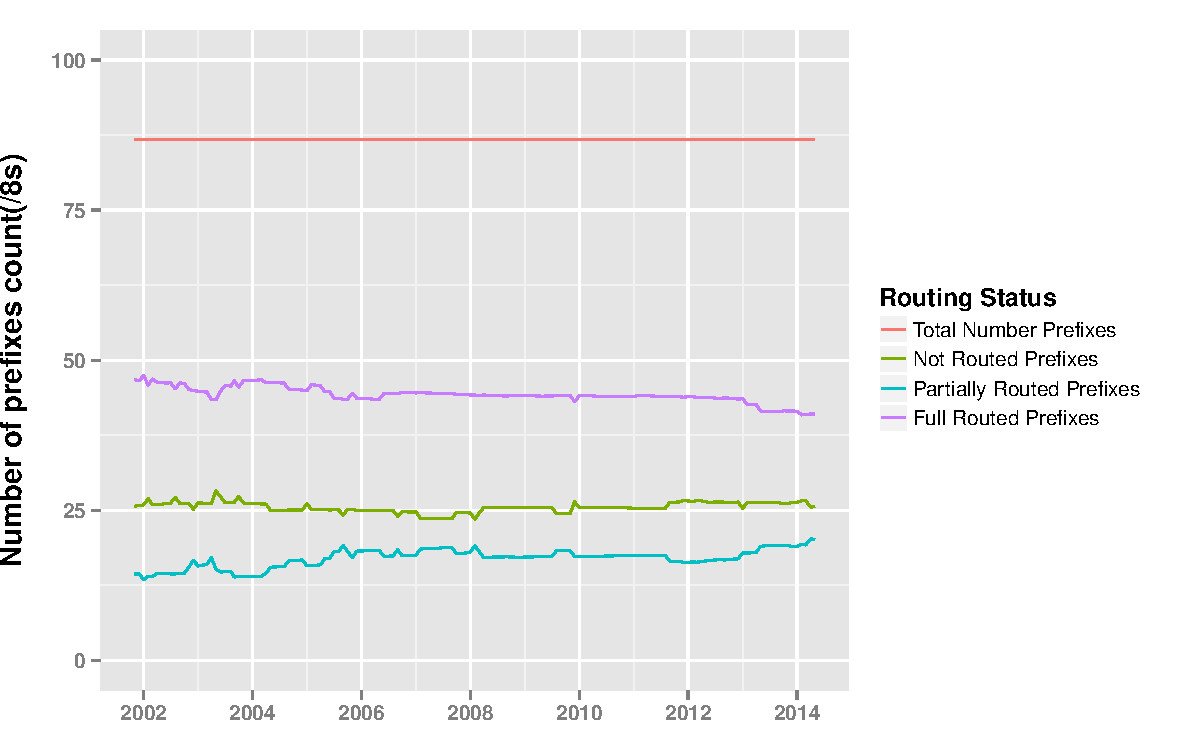
\includegraphics[scale=0.35]{routeStatusOld8.pdf}
\caption{Amount of address space of allocated prefixes, allocated before 1997, that is being advertised in BGP in /8s, according to prefixes routing status}
\label{fig:routingStatusOld8}
\end{figure}

To infer about the quantity of addresses that we are speaking about we use Figure \ref{fig:routingStatusOld8}. We can see that, although in the previous graphic the amount of not routed prefixes is higher than the full routed ones, the number of blocks of addresses being full routed is the double as the amount of addresses not routed. Also the number of partially routed addresses is almost as much as the not routed ones. Still with a value of around 25 /8s the number of not routed addresses is surprisingly high. To understand the difference between the old allocations and new allocations we can observe Figure \ref{fig:routingStatusNew}.

\begin{figure}[!h]
\centering
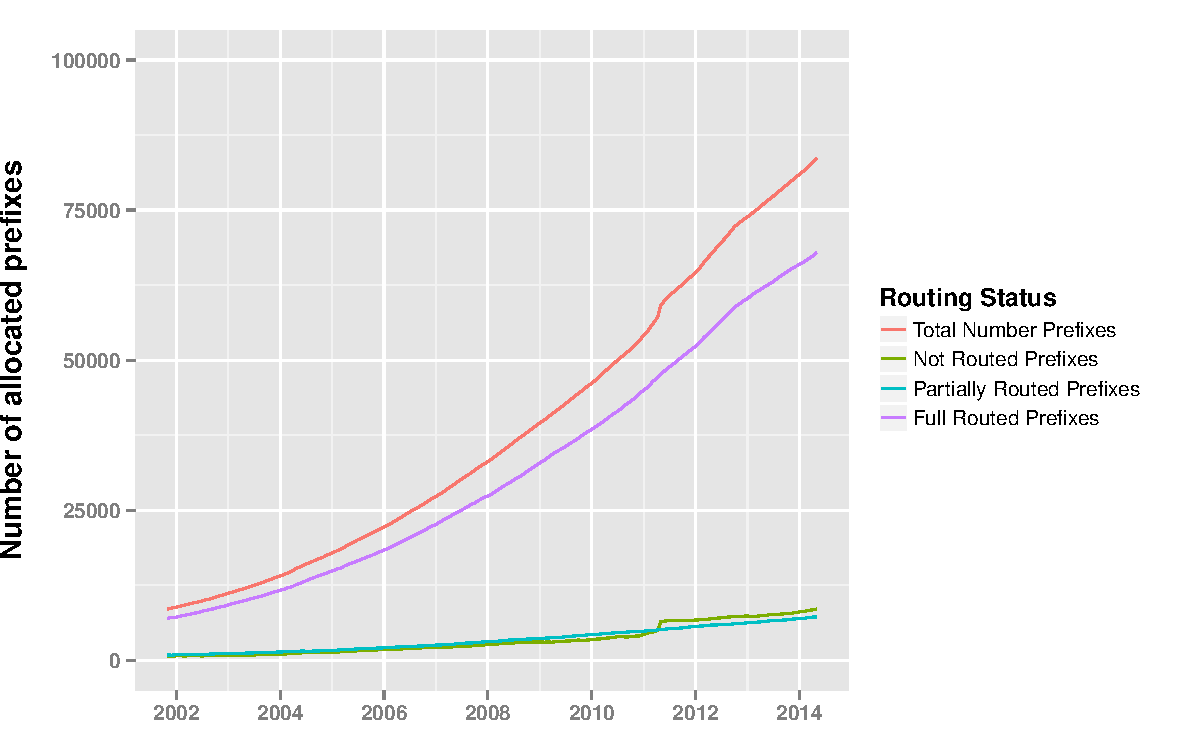
\includegraphics[scale=0.35]{routeStatusNew.pdf}
\caption{Number of allocated prefixes, allocated after 1997, that are being advertised in BGP and their routing status}
\label{fig:routingStatusNew}
\end{figure}

We can immediately notice huge differences between Figure \ref{fig:routingStatusNew} and Figure \ref{fig:routingStatusOld}. Here the number of full routed prefixes rise in accordance to the total of allocated prefixes and is clearly higher than the number of not routed prefixes. The number of partially routed prefixes and not routed prefixes grow together and with a smalll pace, just reaching less than 12000 in 2014 while the number of full routed prefixes is around 70 000. We can say that the number of not routed prefixes in the global view is mostly from allocated prefixes before 1997.


\begin{figure}[!h]
\centering
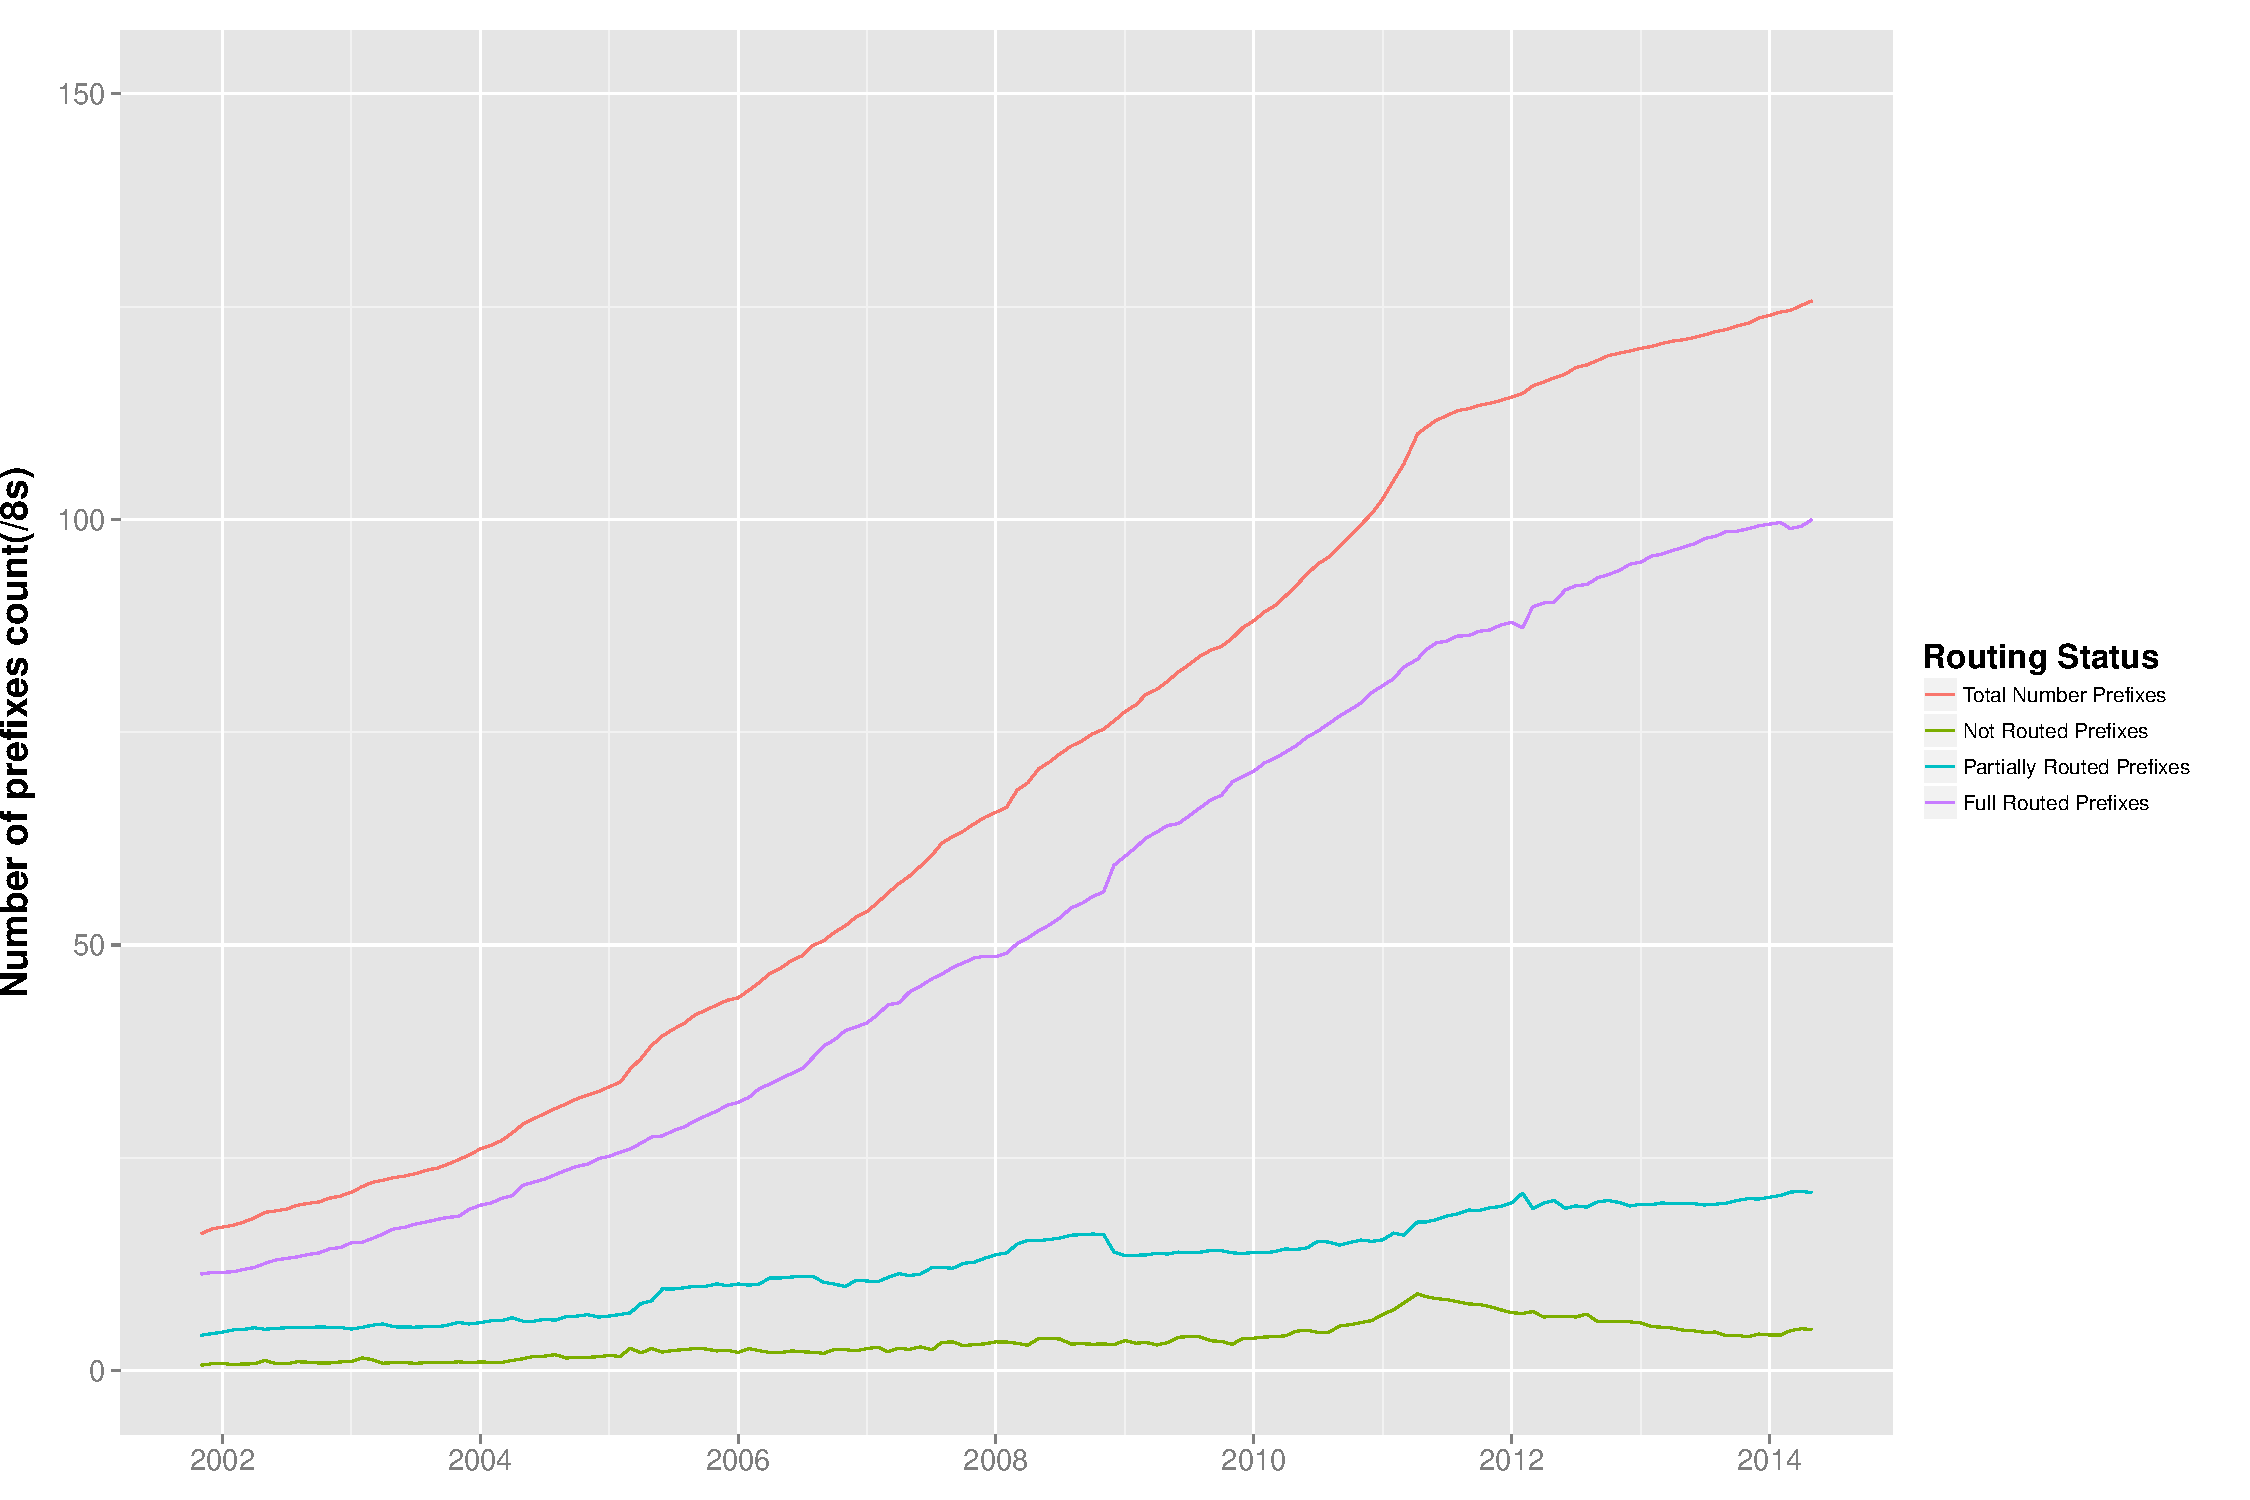
\includegraphics[scale=0.35]{routeStatusNew8.pdf}
\caption{Amount of address space of allocated prefixes, allocated after 1997, that is being advertised in BGP in /8s, according to prefixes routing status}
\label{fig:routingStatusNew8}
\end{figure}

In Figure \ref{fig:routingStatusNew8} we see the amount of addresses in terms of /8s. We continue to see that the amount of full routed is following the number of total allocated ones and is increasing rapidly, alghouth slowing down in the last years as a result of IPv4 adress exaushtion. The number of partially routed addresses is higher than the not routed ones and here the number of not routed is quite small, around 5 /8s. We can say that the contribution to not routed prefixes in the global view is being made by prefixes allocated before 1997. Although we cannot assure that the IPv4 addresses in these blocks are not being used, it is certainly an indicating that most probably there are plenty of IPv4 addresses in the old allocated prefixes can be be used for future use and to further allow the use of IPv4.

\begin{figure}[!h]
\centering
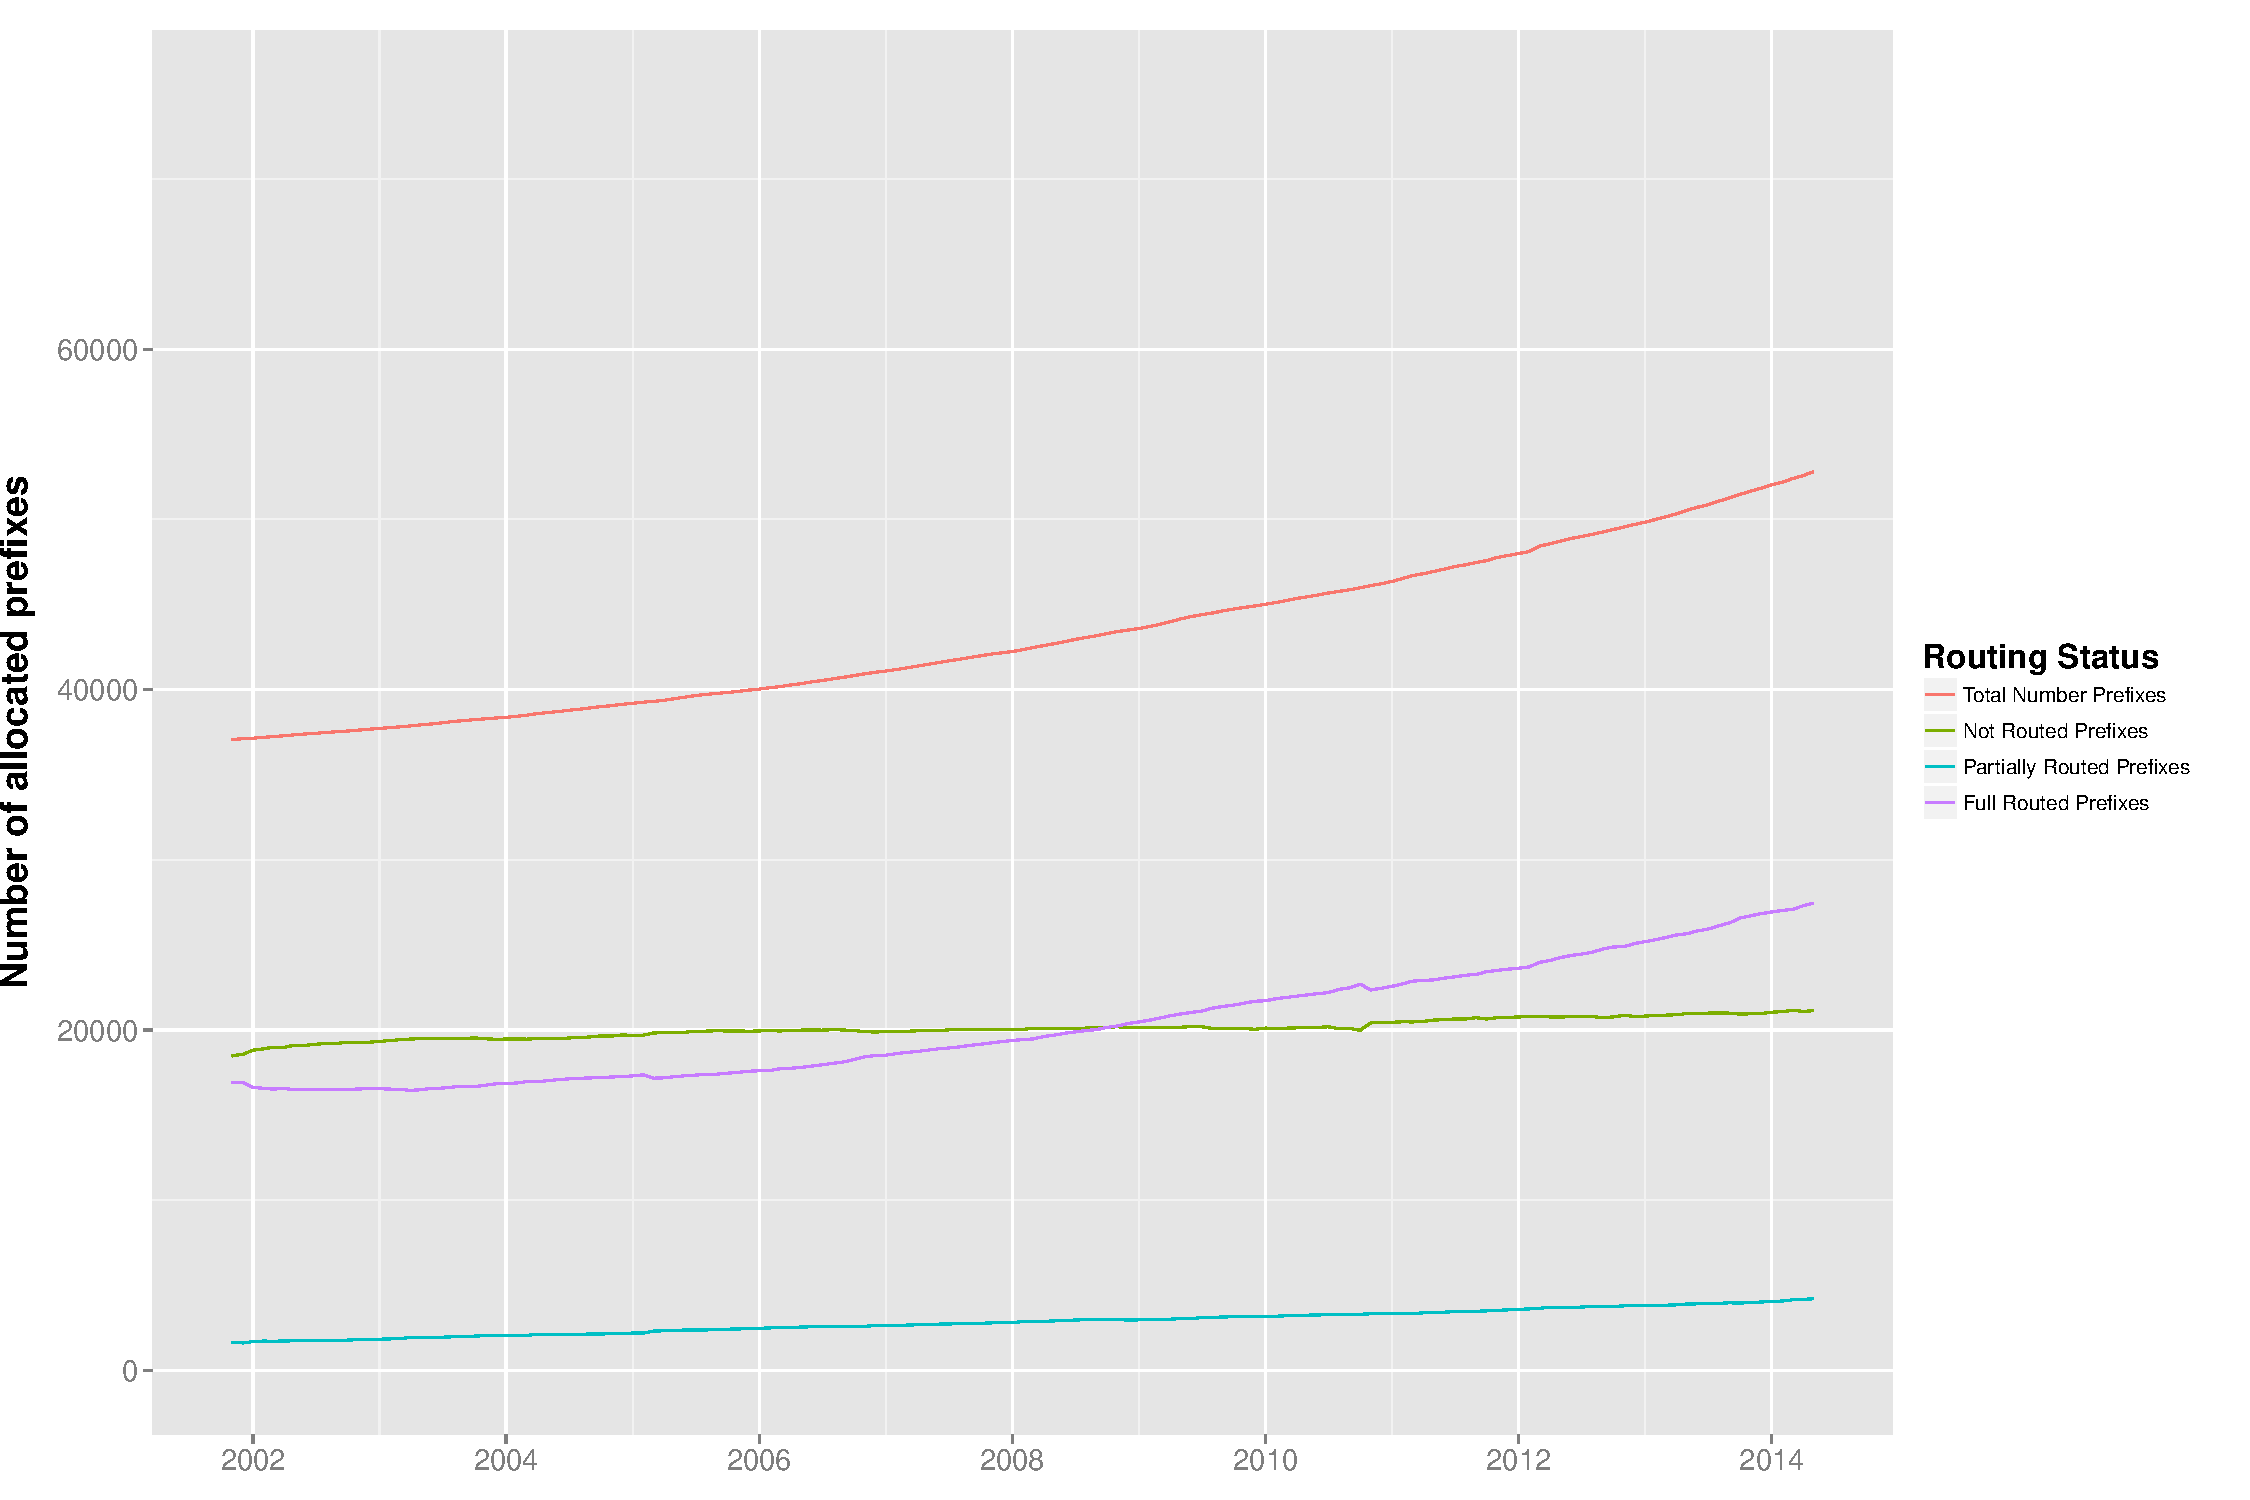
\includegraphics[scale=0.35]{routeStatusArin.pdf}
\caption{Number of allocated prefixes, in ARIN, that are being advertised in BGP and their routing status}
\label{fig:routingStatusArin}
\end{figure}

Having studied the allocated prefixes before and after 1997, we decided to infer on how is the behaviour for each of the RIRs. In Figure \ref{fig:routingStatusArin} are represented the results for ARIN.  
While the number of partially routed prefixes is very low, around 2000 e 2001 the number of not routed prefixes and full routed prefixes is much higher and almost the same, around 18000 for the not routed prefixes and 17000 for full routed prefixes. In 2014 the number of full routed prefixes increased in the same way as the number of total allocated prefixes increased while the number of not routed prefixes remained constant. Beggining of 2014 we could observe 21000 prefixes that were not routed and 27000 full routed. Partially routed prefixes remained low with around 4000. The distribution in ARIN was expected to be similar to the old allocations as most of these old allocations belong exactly to ARIN. 

\begin{figure}[!h]
\centering
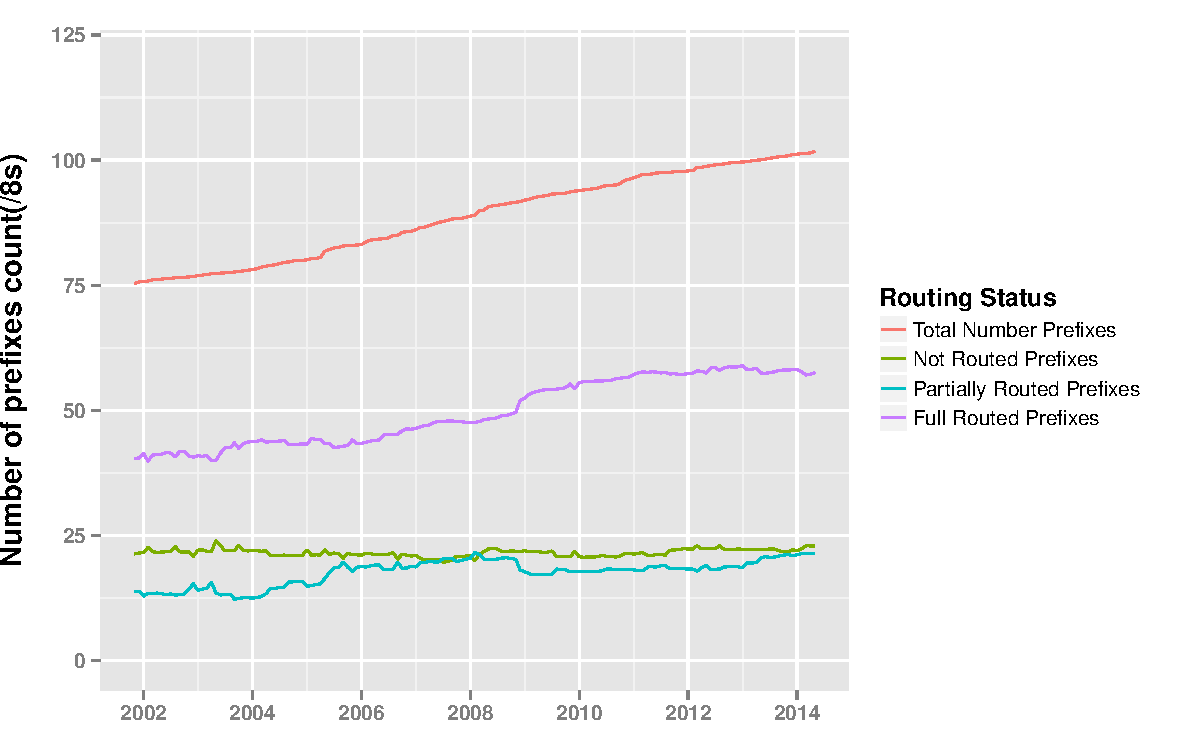
\includegraphics[scale=0.35]{routeStatusArin8.pdf}
\caption{Amount of address space of allocated prefixes, in ARIN, that is being advertised in BGP in /8s, according to prefixes routing status}
\label{fig:routingStatusArin8}
\end{figure}

In Figure \ref{fig:routingStatusArin8} are represented the count of prefixes in /8s. We can see a trend similar to the old allocations, as expected, due to the reasons explained above. We can also notice that the number of full routed prefixes has been increasing. The count of partially routed and not routed prefixes is very similar and we can notice again that although many more prefixes in number were not routed than partially routed, when we take into account the number of addresses the value is very similar. 

The second RIR we studied was AFRINIC, represented in Figure \ref{fig:routingStatusAfrinic}. We can notice that the number of allocated prefixes increased at a high rate and the number of full routed prefixes increased accordingly. As the number of not routed prefixes remaining constant along the time period and the number of partly routed prefixes also had this trend we can assume that the majority of new prefixes being allocated was also fully routed. Still the number of allocated prefixes was much smaller in AFRINIC, with 2500 prefixes in comparison to  around 130 000 globally. 

\begin{figure}[!h]
\centering
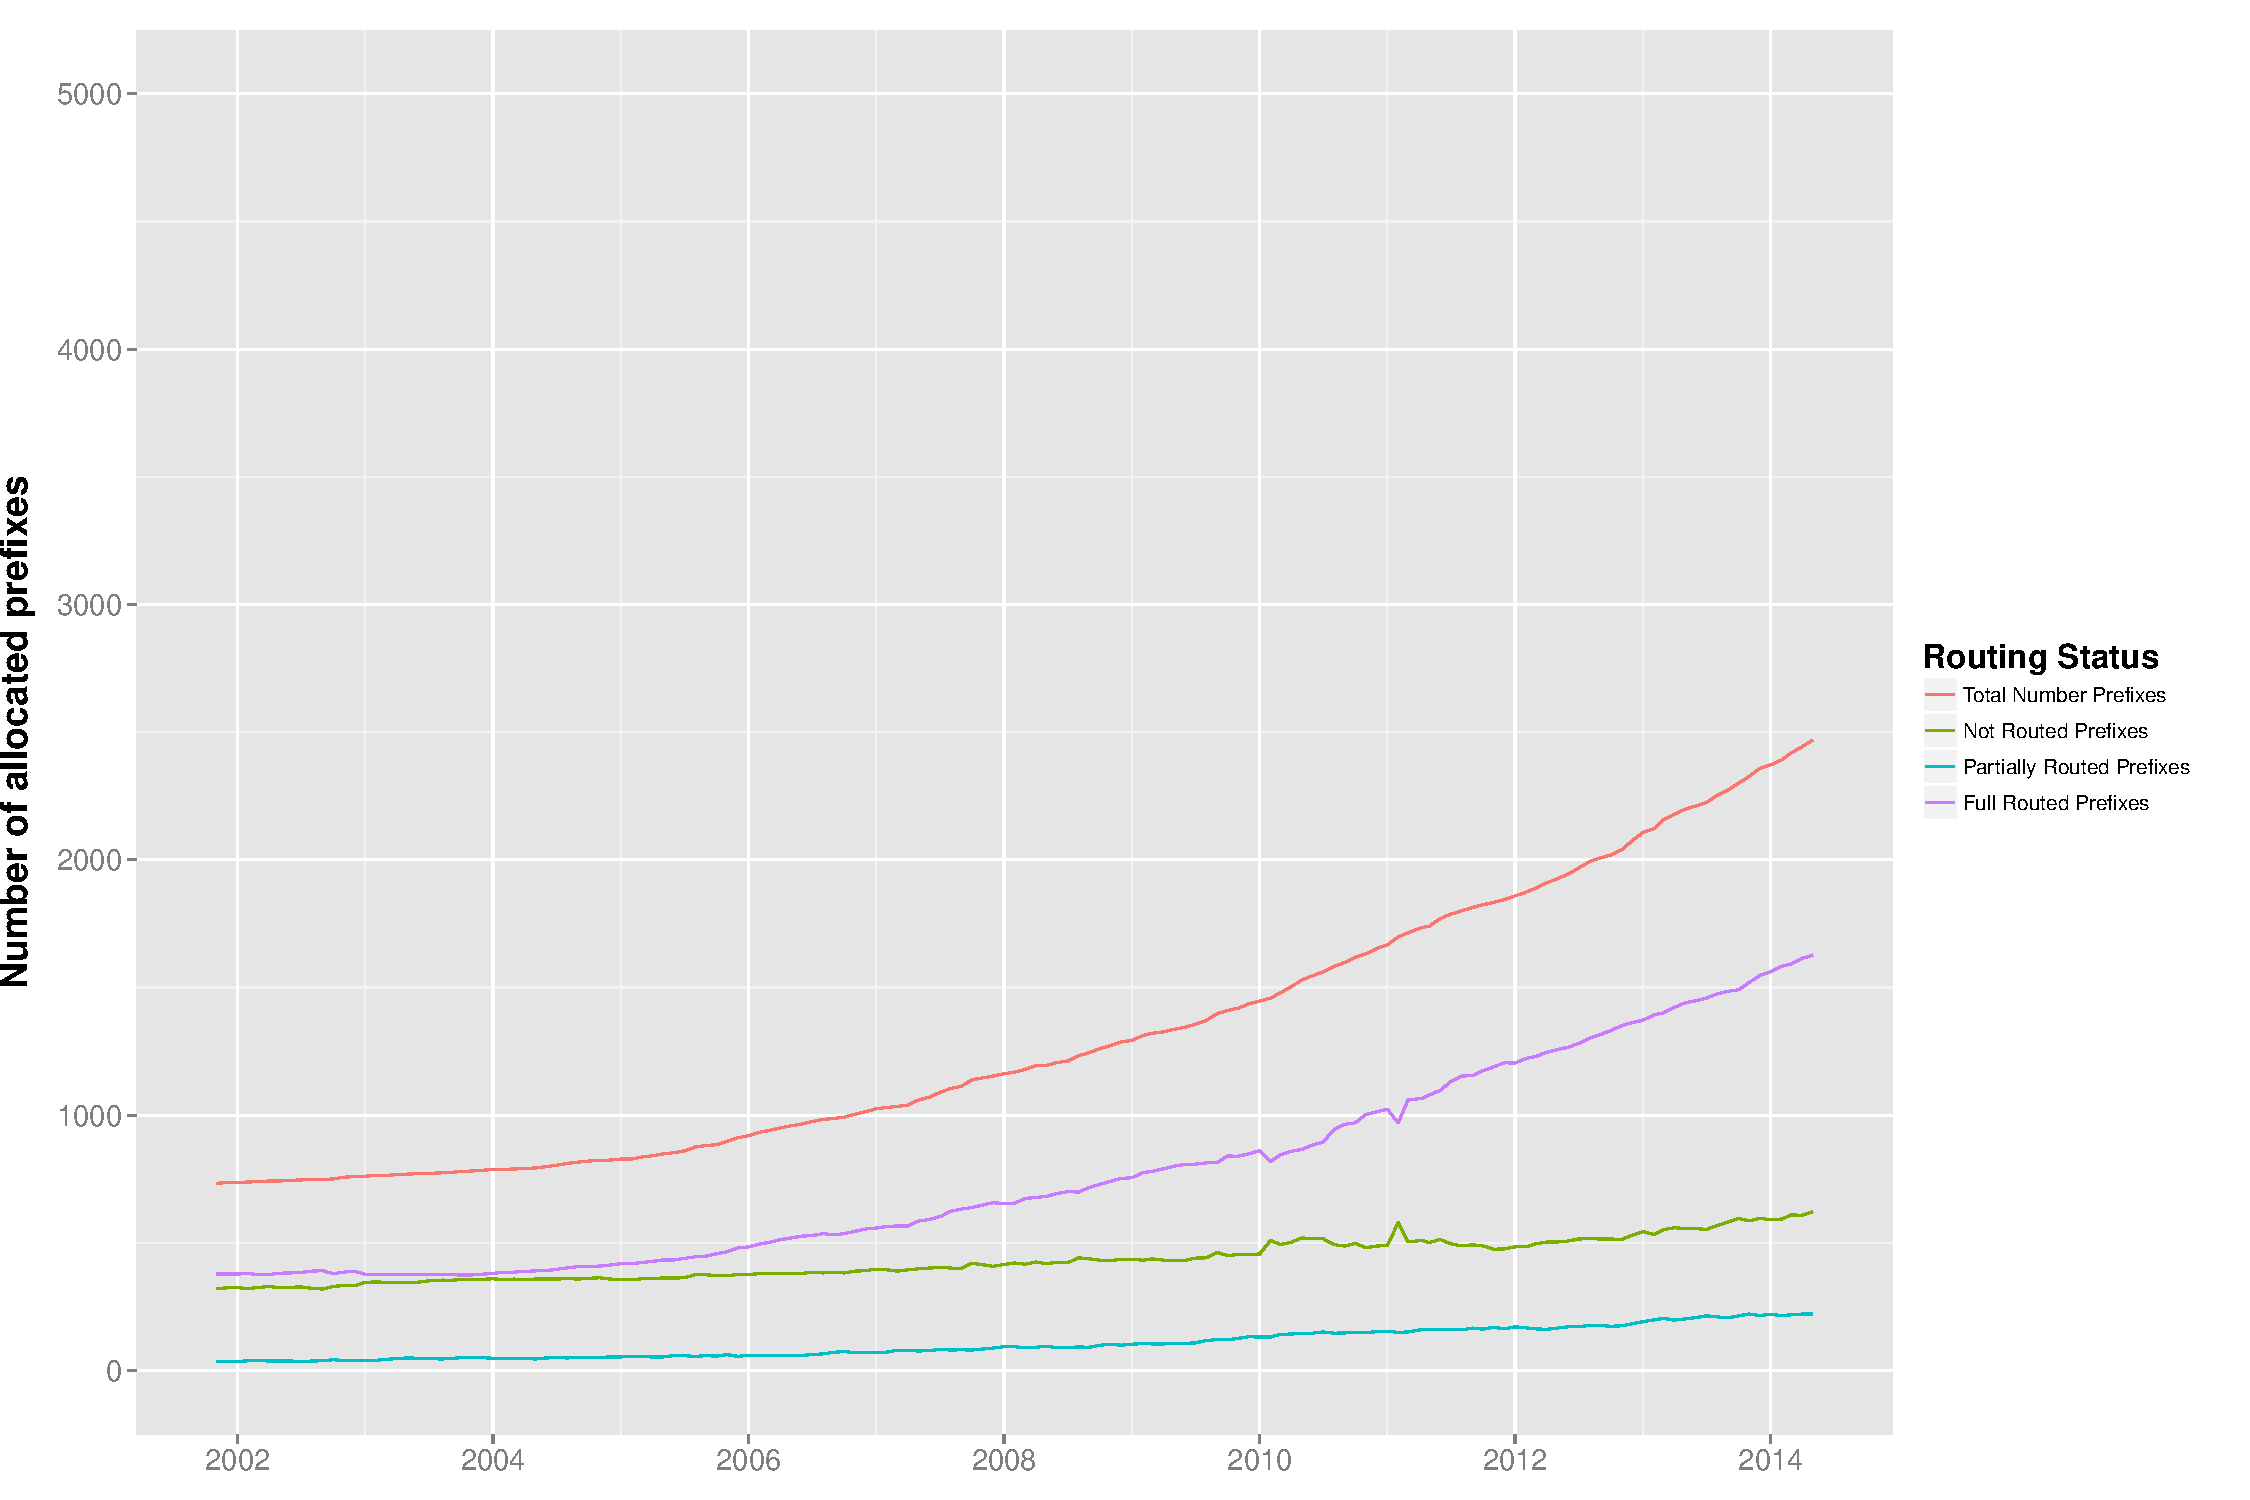
\includegraphics[scale=0.35]{routeStatusAfrinic.pdf}
\caption{Number of allocated prefixes, in AFRINIC, that are being advertised in BGP and their routing status}
\label{fig:routingStatusAfrinic}
\end{figure}

When we analize the count of prefixes in /8s shown in Figure \ref{fig:routingStatusAfrinic8}, we can see that the amount of address space allocated to AFRINIC is very small, only four /8s. The only difference we can see here is that the amount of address space that is not being routed is smaller than the amount of address space that is partially routed, since 2012. 

\begin{figure}[!h]
\centering
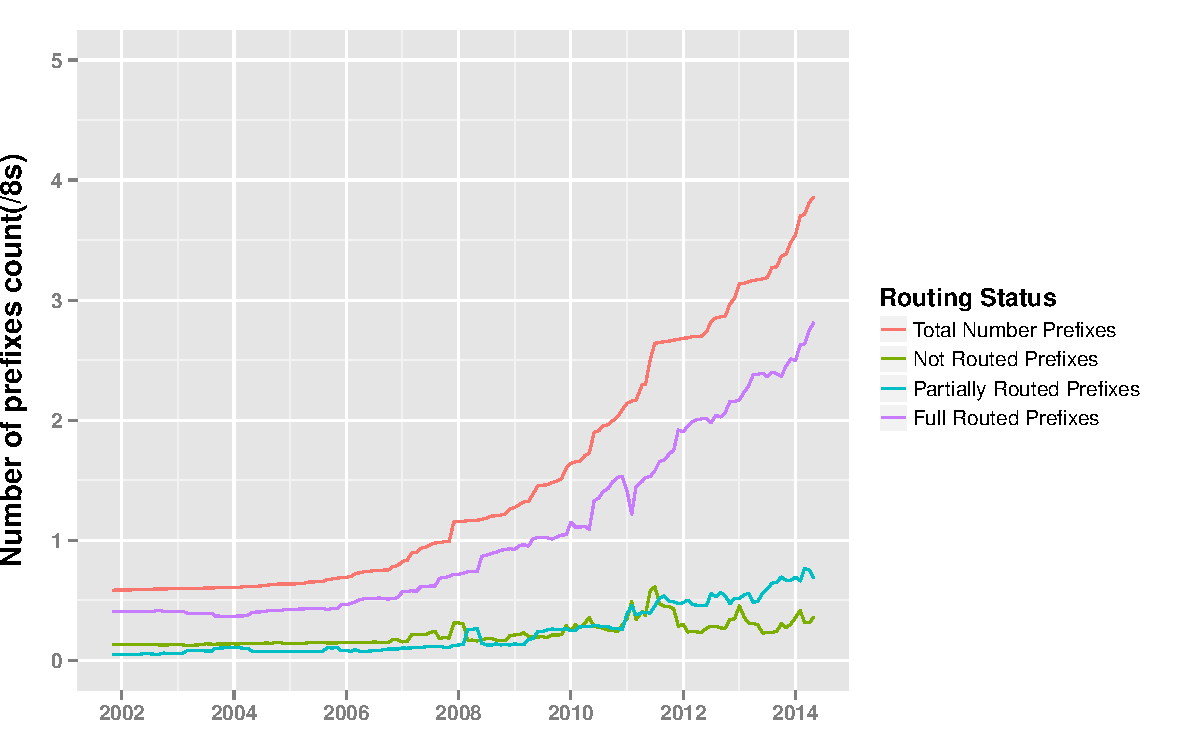
\includegraphics[scale=0.35]{routeStatusAfrinic8.pdf}
\caption{Amount of address space of allocated prefixes, in AFRINIC, that is being advertised in BGP in /8s, according to prefixes routing status}
\label{fig:routingStatusAfrinic8}
\end{figure}

The analysis of APNIC is shown in Figure \ref{fig:routingStatusApnic}. We can again notice the increase of allocated prefixes, although at a small rate, and the number of full routed prefixes follows this trend. The total number of allocated prefixes is around 24 000. We can see that the number of partially routed prefixes remained approximately constant as well as the number of not routed ones. Exception in 2011 where we can see a peak of allocated prefixes that reflects itself in the number of not routed prefixes, indicating that the prefixes in this peak were not routed.  

\begin{figure}[!h]
\centering
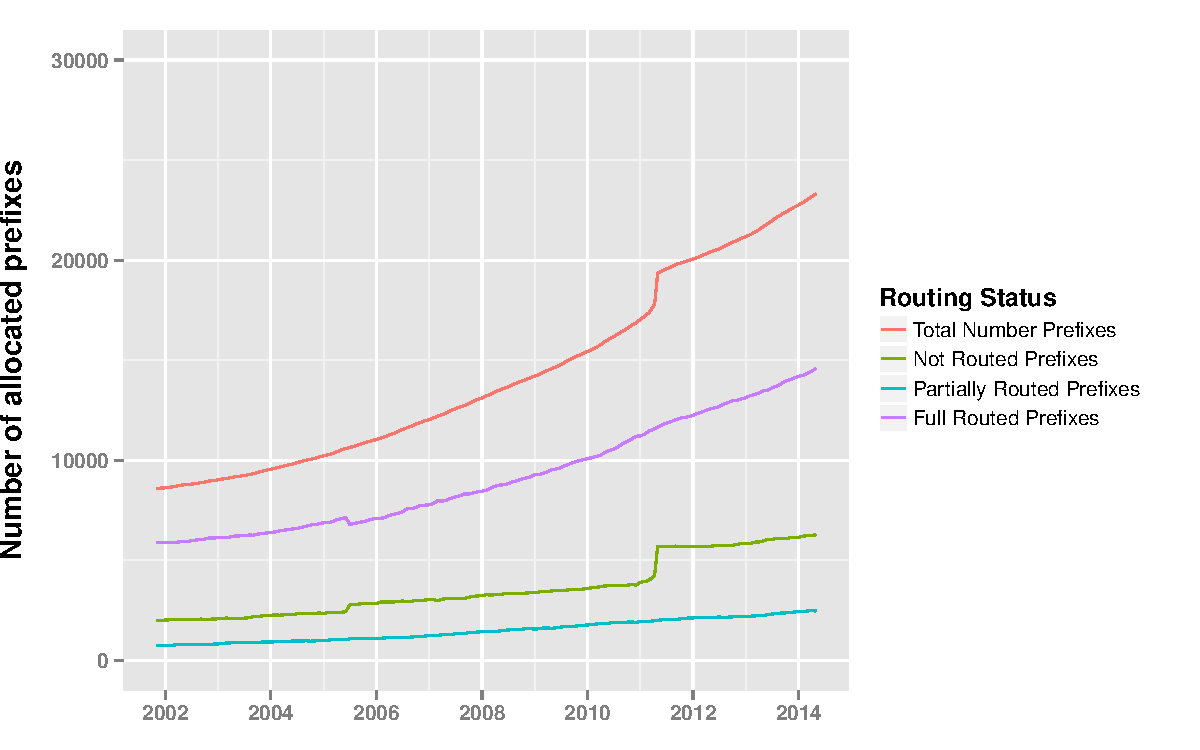
\includegraphics[scale=0.35]{routeStatusApnic.pdf}
\caption{Number of allocated prefixes, in APNIC, that are being advertised in BGP and their routing status}
\label{fig:routingStatusApnic}
\end{figure}

Looking at the count of prefixes in /8s, Figure \ref{fig:routingStatusApnic8}, we see that since 2011 the amount of address remained pratically constant although we see in the previous Figure that there were still prefixes being allocated. We can assume that this is due to the change of policy in allocations that APNIC implemented after reaching the last /8, where small blocks of addresses started being allocated. We can also see, since 2011, that while the amount of address space being partially routed or fully routed increased, the amount of not routed address space decreased.

\begin{figure}[!h]
\centering
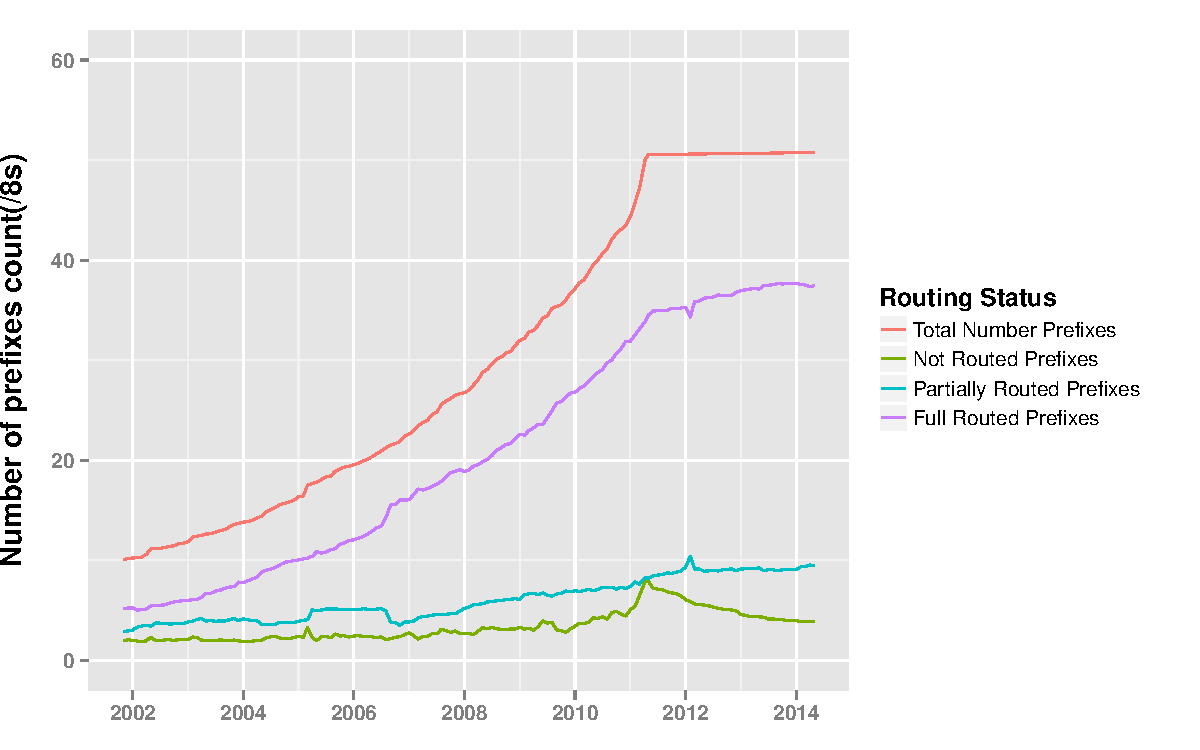
\includegraphics[scale=0.35]{routeStatusApnic8.pdf}
\caption{Amount of address space of allocated prefixes, in APNIC, that is being advertised in BGP in /8s, according to prefixes routing status}
\label{fig:routingStatusApnic8}
\end{figure}

In Figure \ref{fig:routingStatusLacnic} it is shown the analisys for LACNIC. We can see an exponential growth in the total number of allocated prefixes and the number of full routed prefixes follows this trend, indicating that the majority of allocated prefixes was also fully routed. On the other hand the number of partially routed prefixes and not routed ones show a very slow rate of increase.

\begin{figure}[!h]
\centering
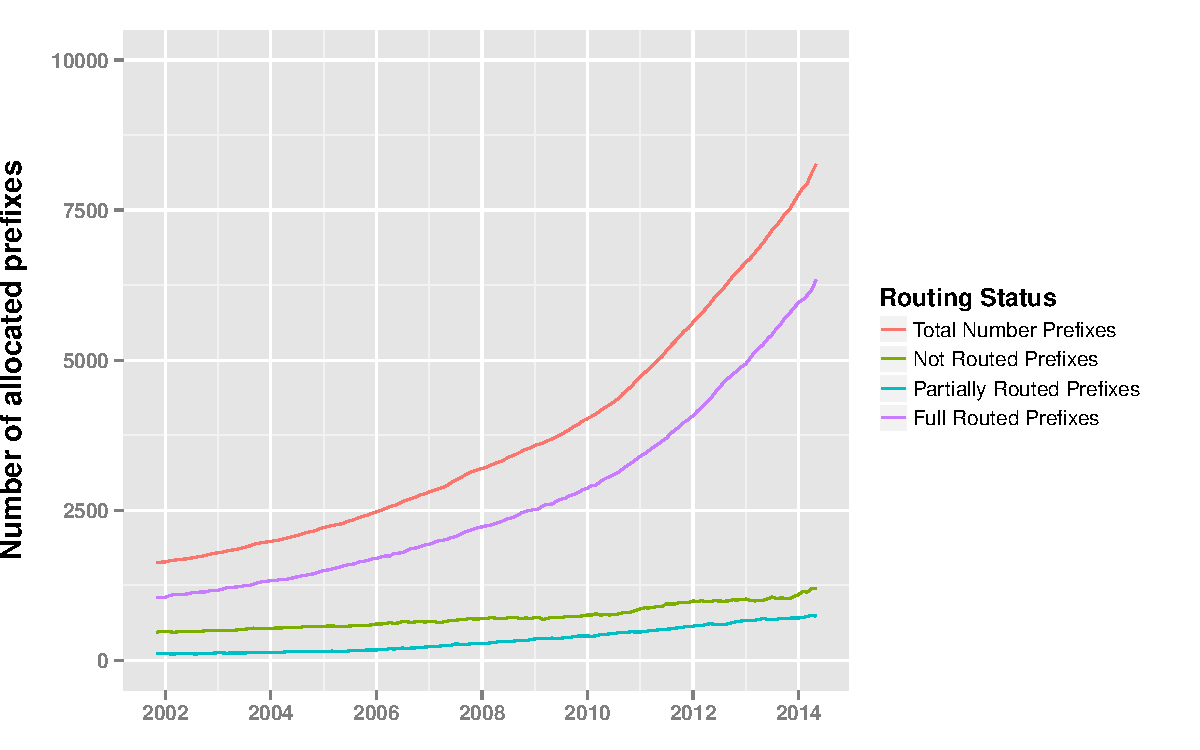
\includegraphics[scale=0.35]{routeStatusLacnic.pdf}
\caption{Number of allocated prefixes, in LACNIC, that are being advertised in BGP and their routing status}
\label{fig:routingStatusLacnic}
\end{figure}

In Figure \ref{fig:routingStatusLacnic8} we have the count of prefixes in /8s. As expected, the amount of address space allocated and fully routed follows the same trend, an exponential increase. The total amount of address space is around eleven /8s. We can also see that the amount of address space that is not routed is almos zero, indicating a high usage of allocated prefixes in the LACNIC region.

\begin{figure}[!h]
\centering
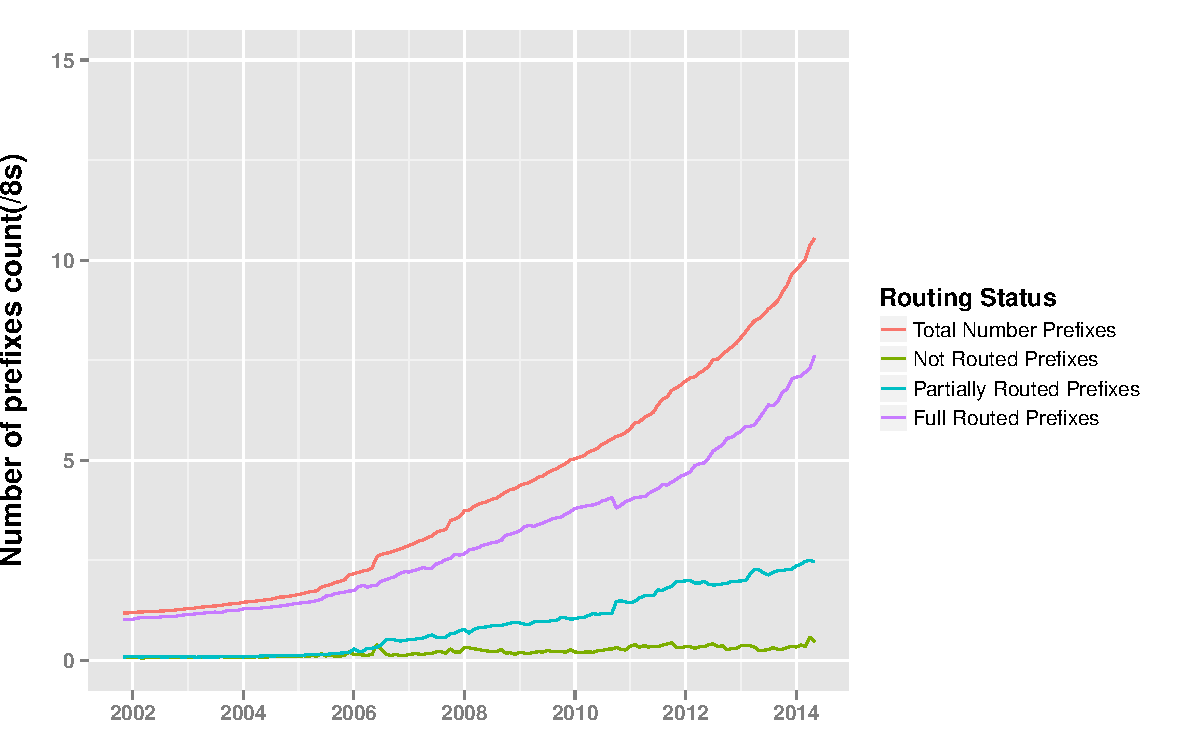
\includegraphics[scale=0.35]{routeStatusLacnic8.pdf}
\caption{Amount of address space of allocated prefixes, in LACNIC, that is being advertised in BGP in /8s, according to prefixes routing status}
\label{fig:routingStatusLacnic8}
\end{figure}

Our last RIR to be analyzed is RIPENCC, which is shown in Figure \ref{fig:routingStatusRipe}. We can see right away that the number of allocated prefixes is high, around 50 000 and it as been a high increasing trend. The number of fully routed prefixes also followed this trend. The number of partially routed prefixes and not routed ones remained constant along the time.

\begin{figure}[!h]
\centering
\begin{subfigure}{.5\textwidth}
  \centering
  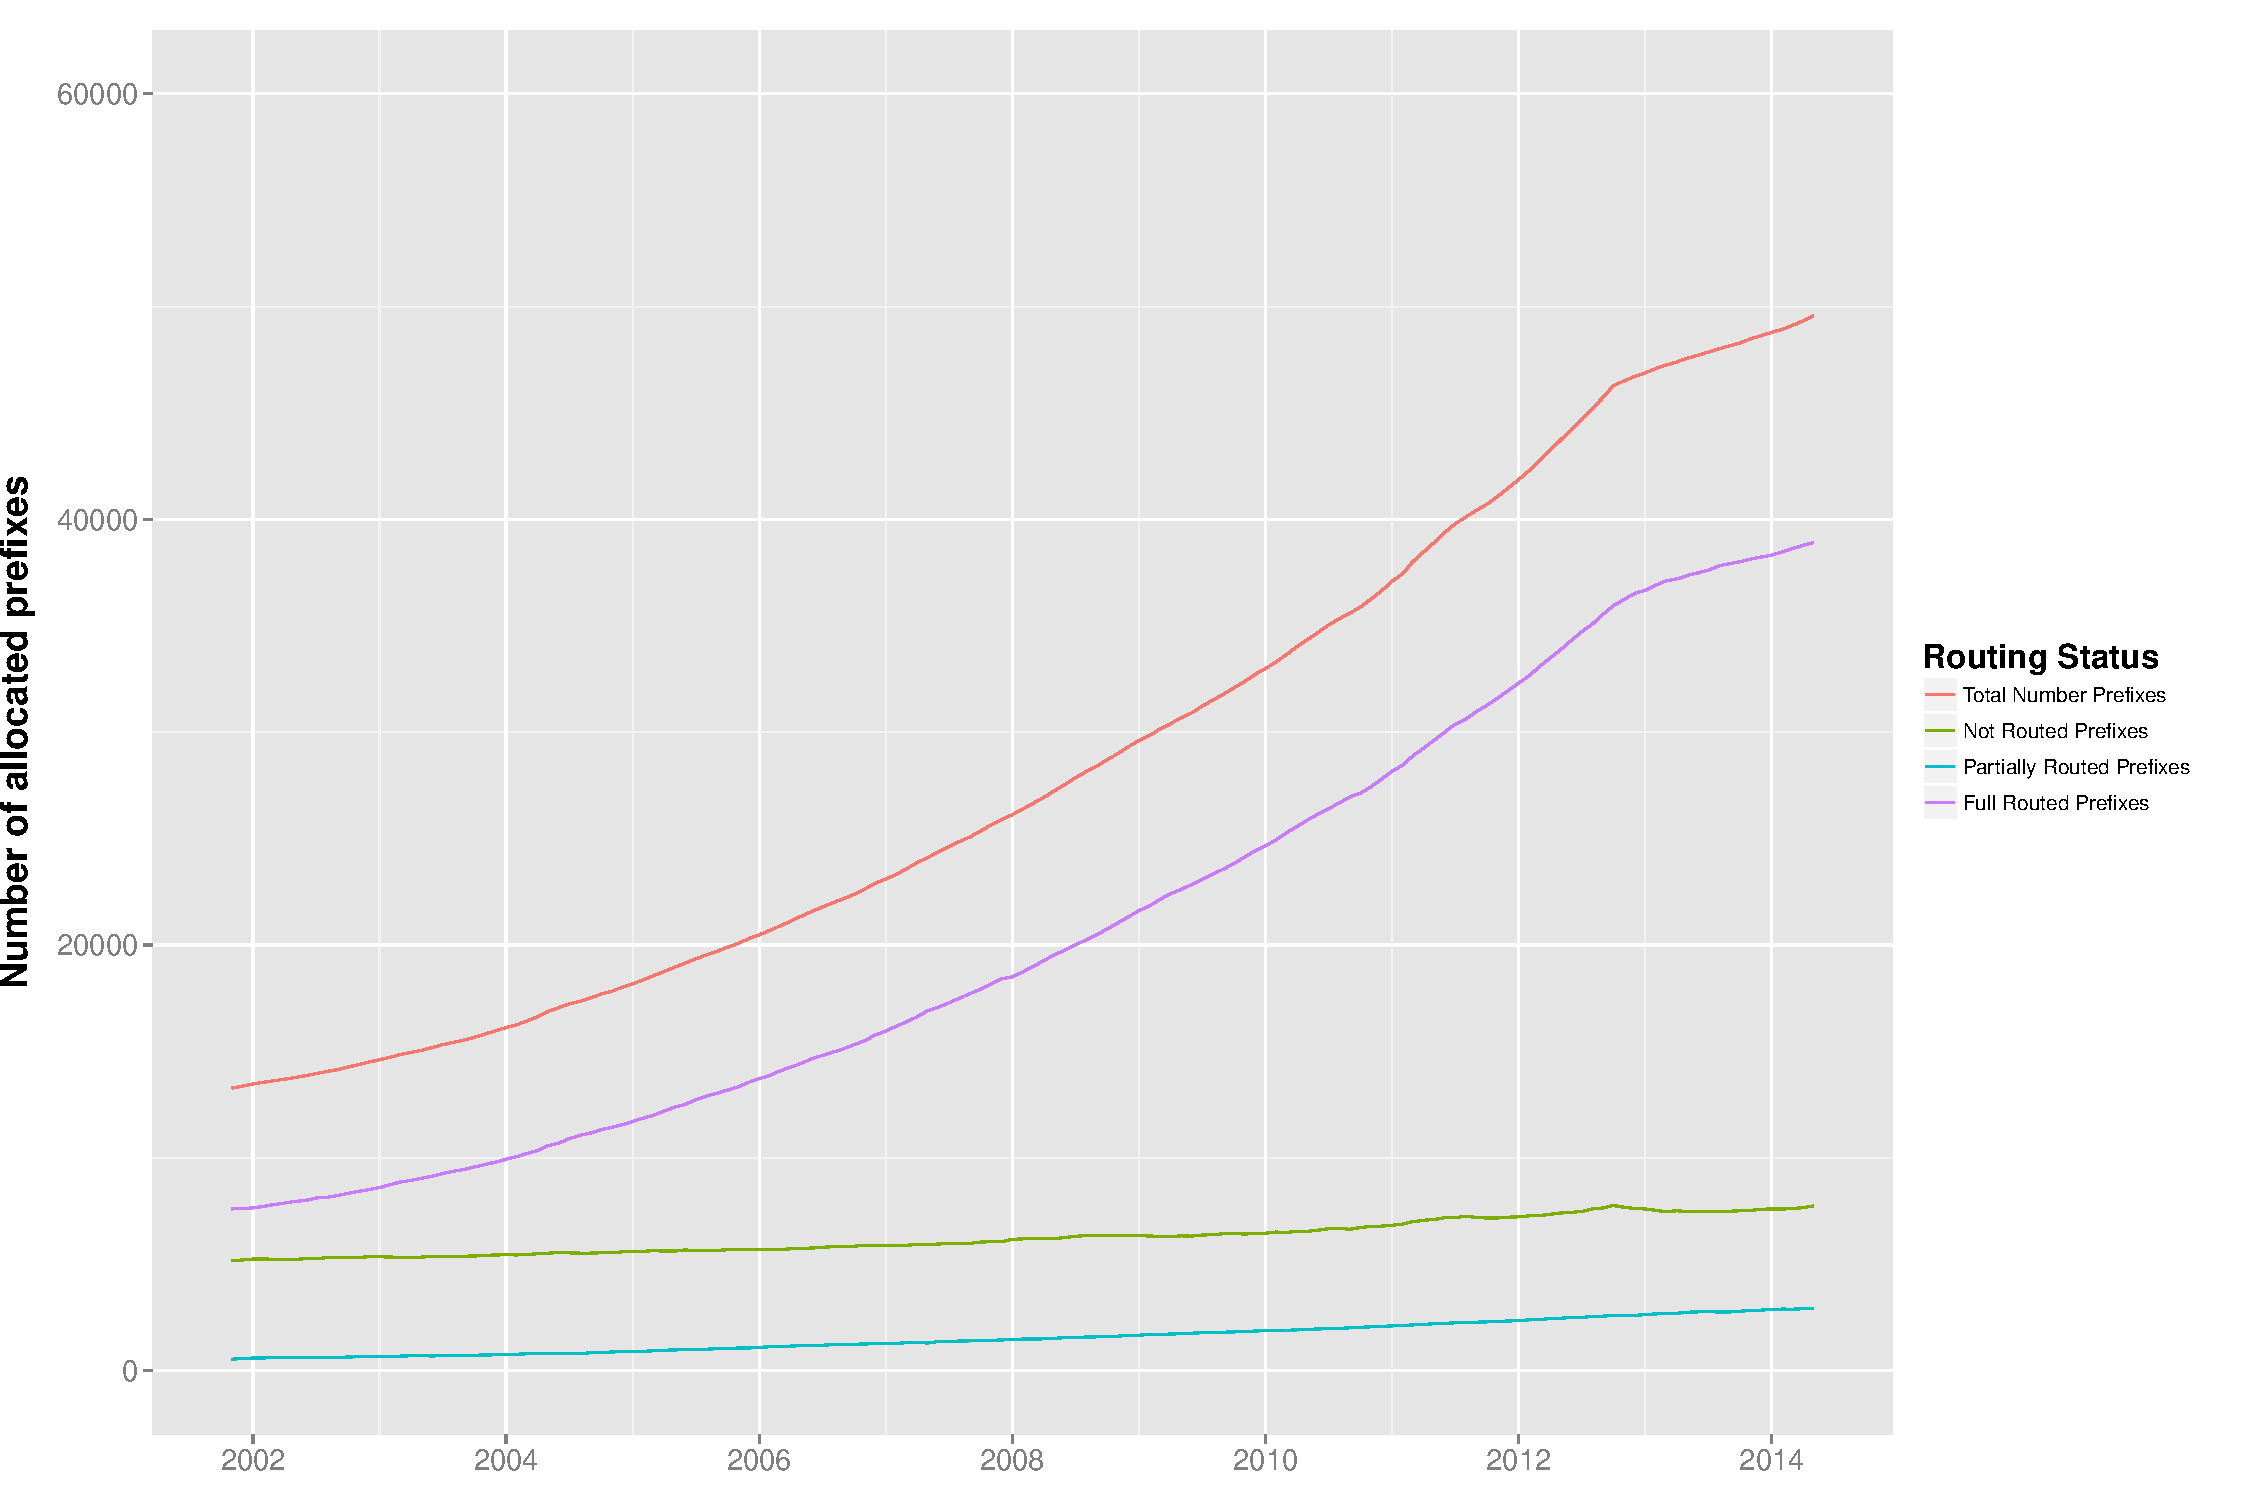
\includegraphics[scale=0.19]{routeStatusRipe.pdf}
  \caption{Number of allocated prefixes, in RIPENCC, that are being advertised in BGP and their routing status}
  \label{fig:routingStatusRipe}
\end{subfigure}%
\begin{subfigure}{.5\textwidth}
  \centering
  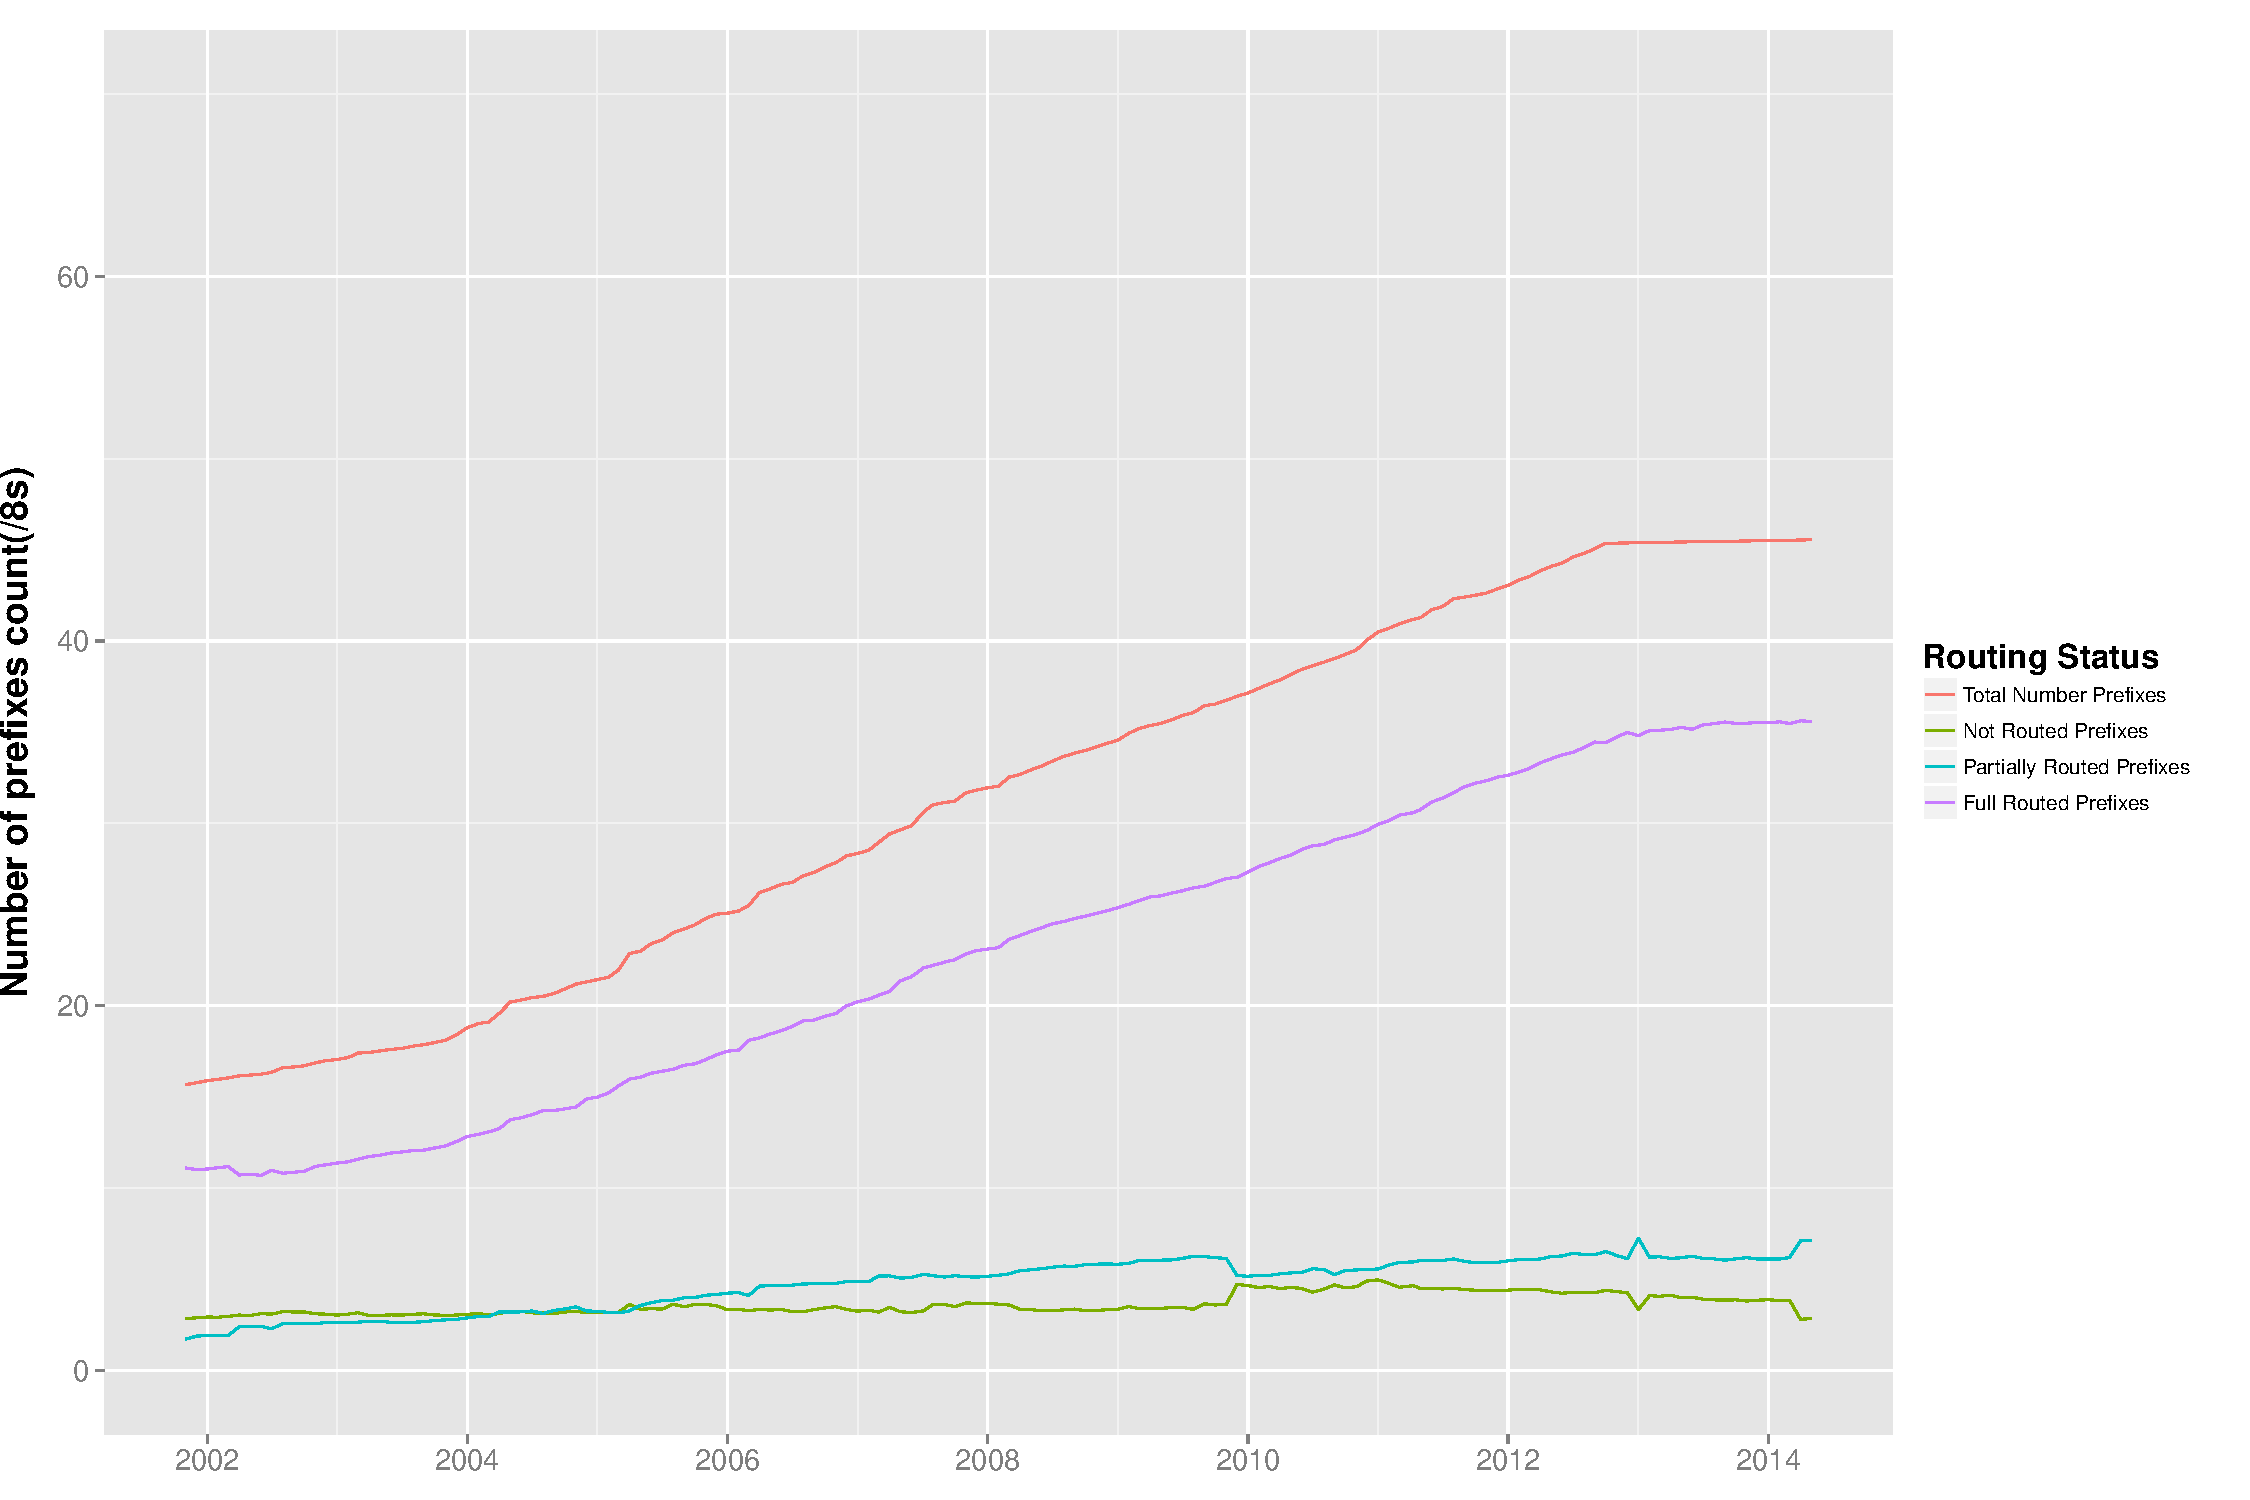
\includegraphics[scale=0.19]{routeStatusRipe8.pdf}
  \caption{Amount of address space of allocated prefixes, in RIPENCC, that is being advertised in BGP in /8s, according to prefixes routing status}
  \label{fig:routingStatusRipe8}
\end{subfigure}
\caption{Observed allocated prefixes in RIPENCC}
\label{fig:test}
\end{figure}


%\begin{figure}[ht!]
%\centering
%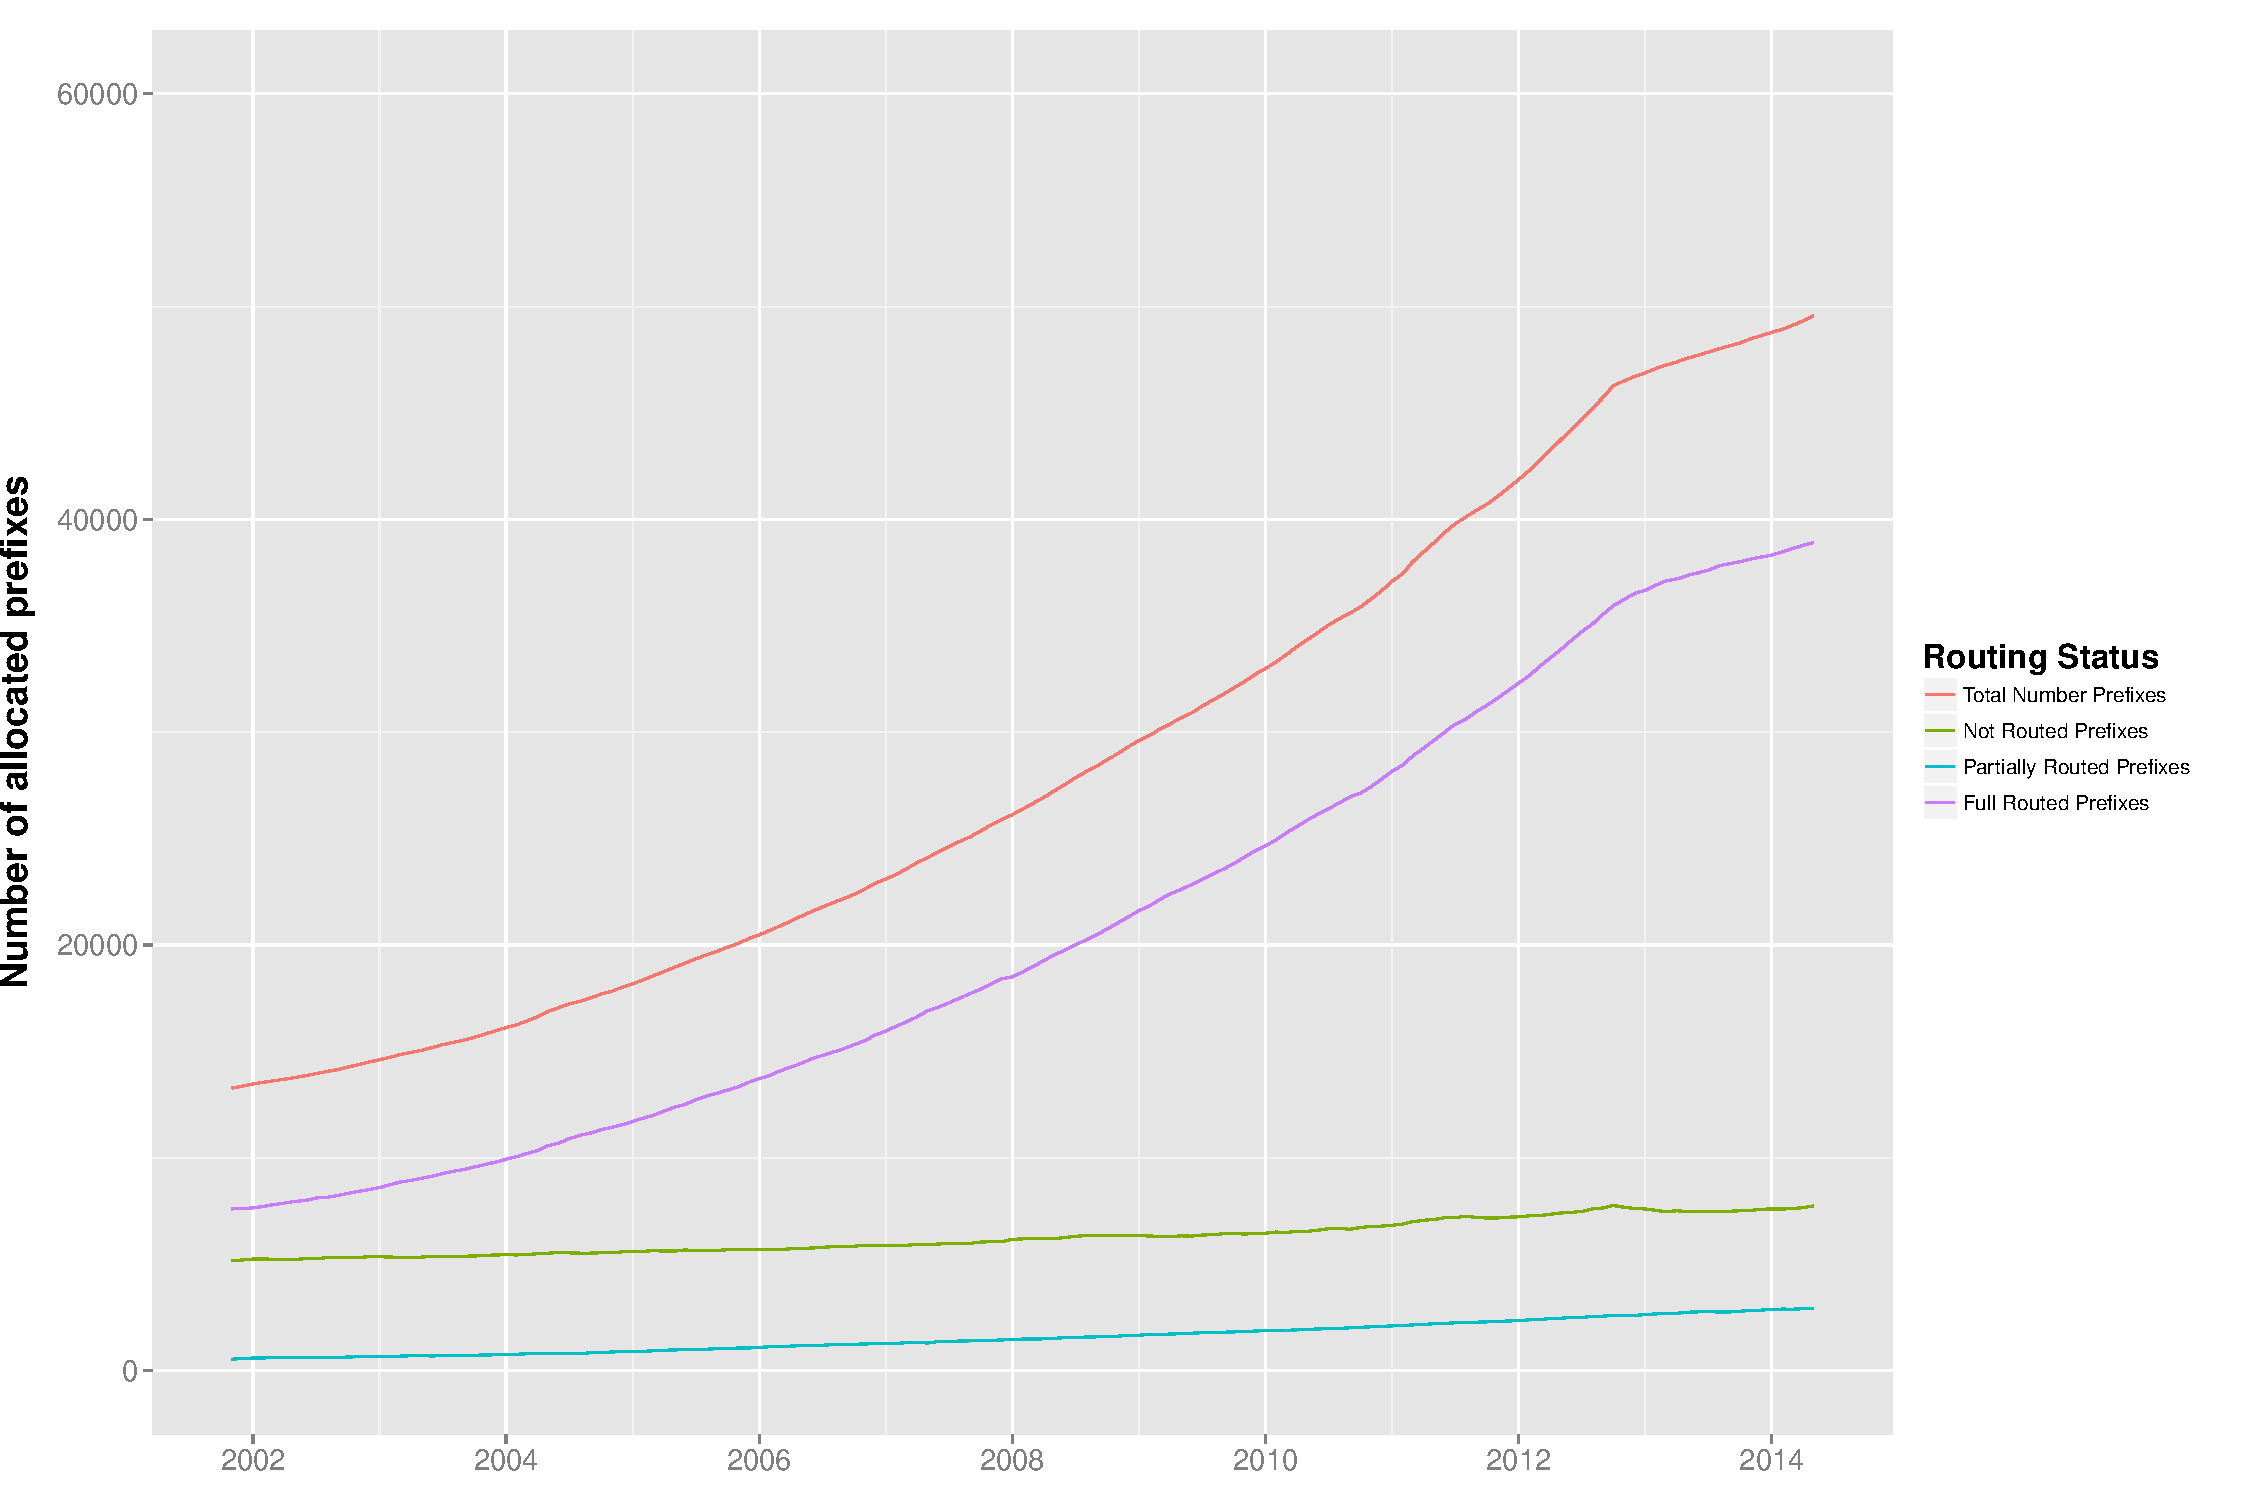
\includegraphics[scale=0.35]{routeStatusRipe.pdf}
%\caption{Number of allocated prefixes, in RIPENCC, that are being advertised in BGP %and their routing status}
%\label{fig:routingStatusRipe}
%\end{figure}

In Figure \ref{fig:routingStatusRipe8} we have the count of prefixes in /8s. We can notice an increasing trend in the amount of allocated address space and the amount of fully routed address space. We notice that since late 2012 this trend changed and remained in an almost constant value. This is due to the fact that RIPENCC reached its final /8 and changed its allocation policy. We notice again that prefixes were still being allocated, but the corresponding address space was low. The amount of partially routed and not routed address space has been somewhat constant, but in recent years we can notice a slight incresing trend in the number of partially routed and a slight decreasing trend in the number of not routed address space.

%\begin{figure}[ht!]
%\centering
%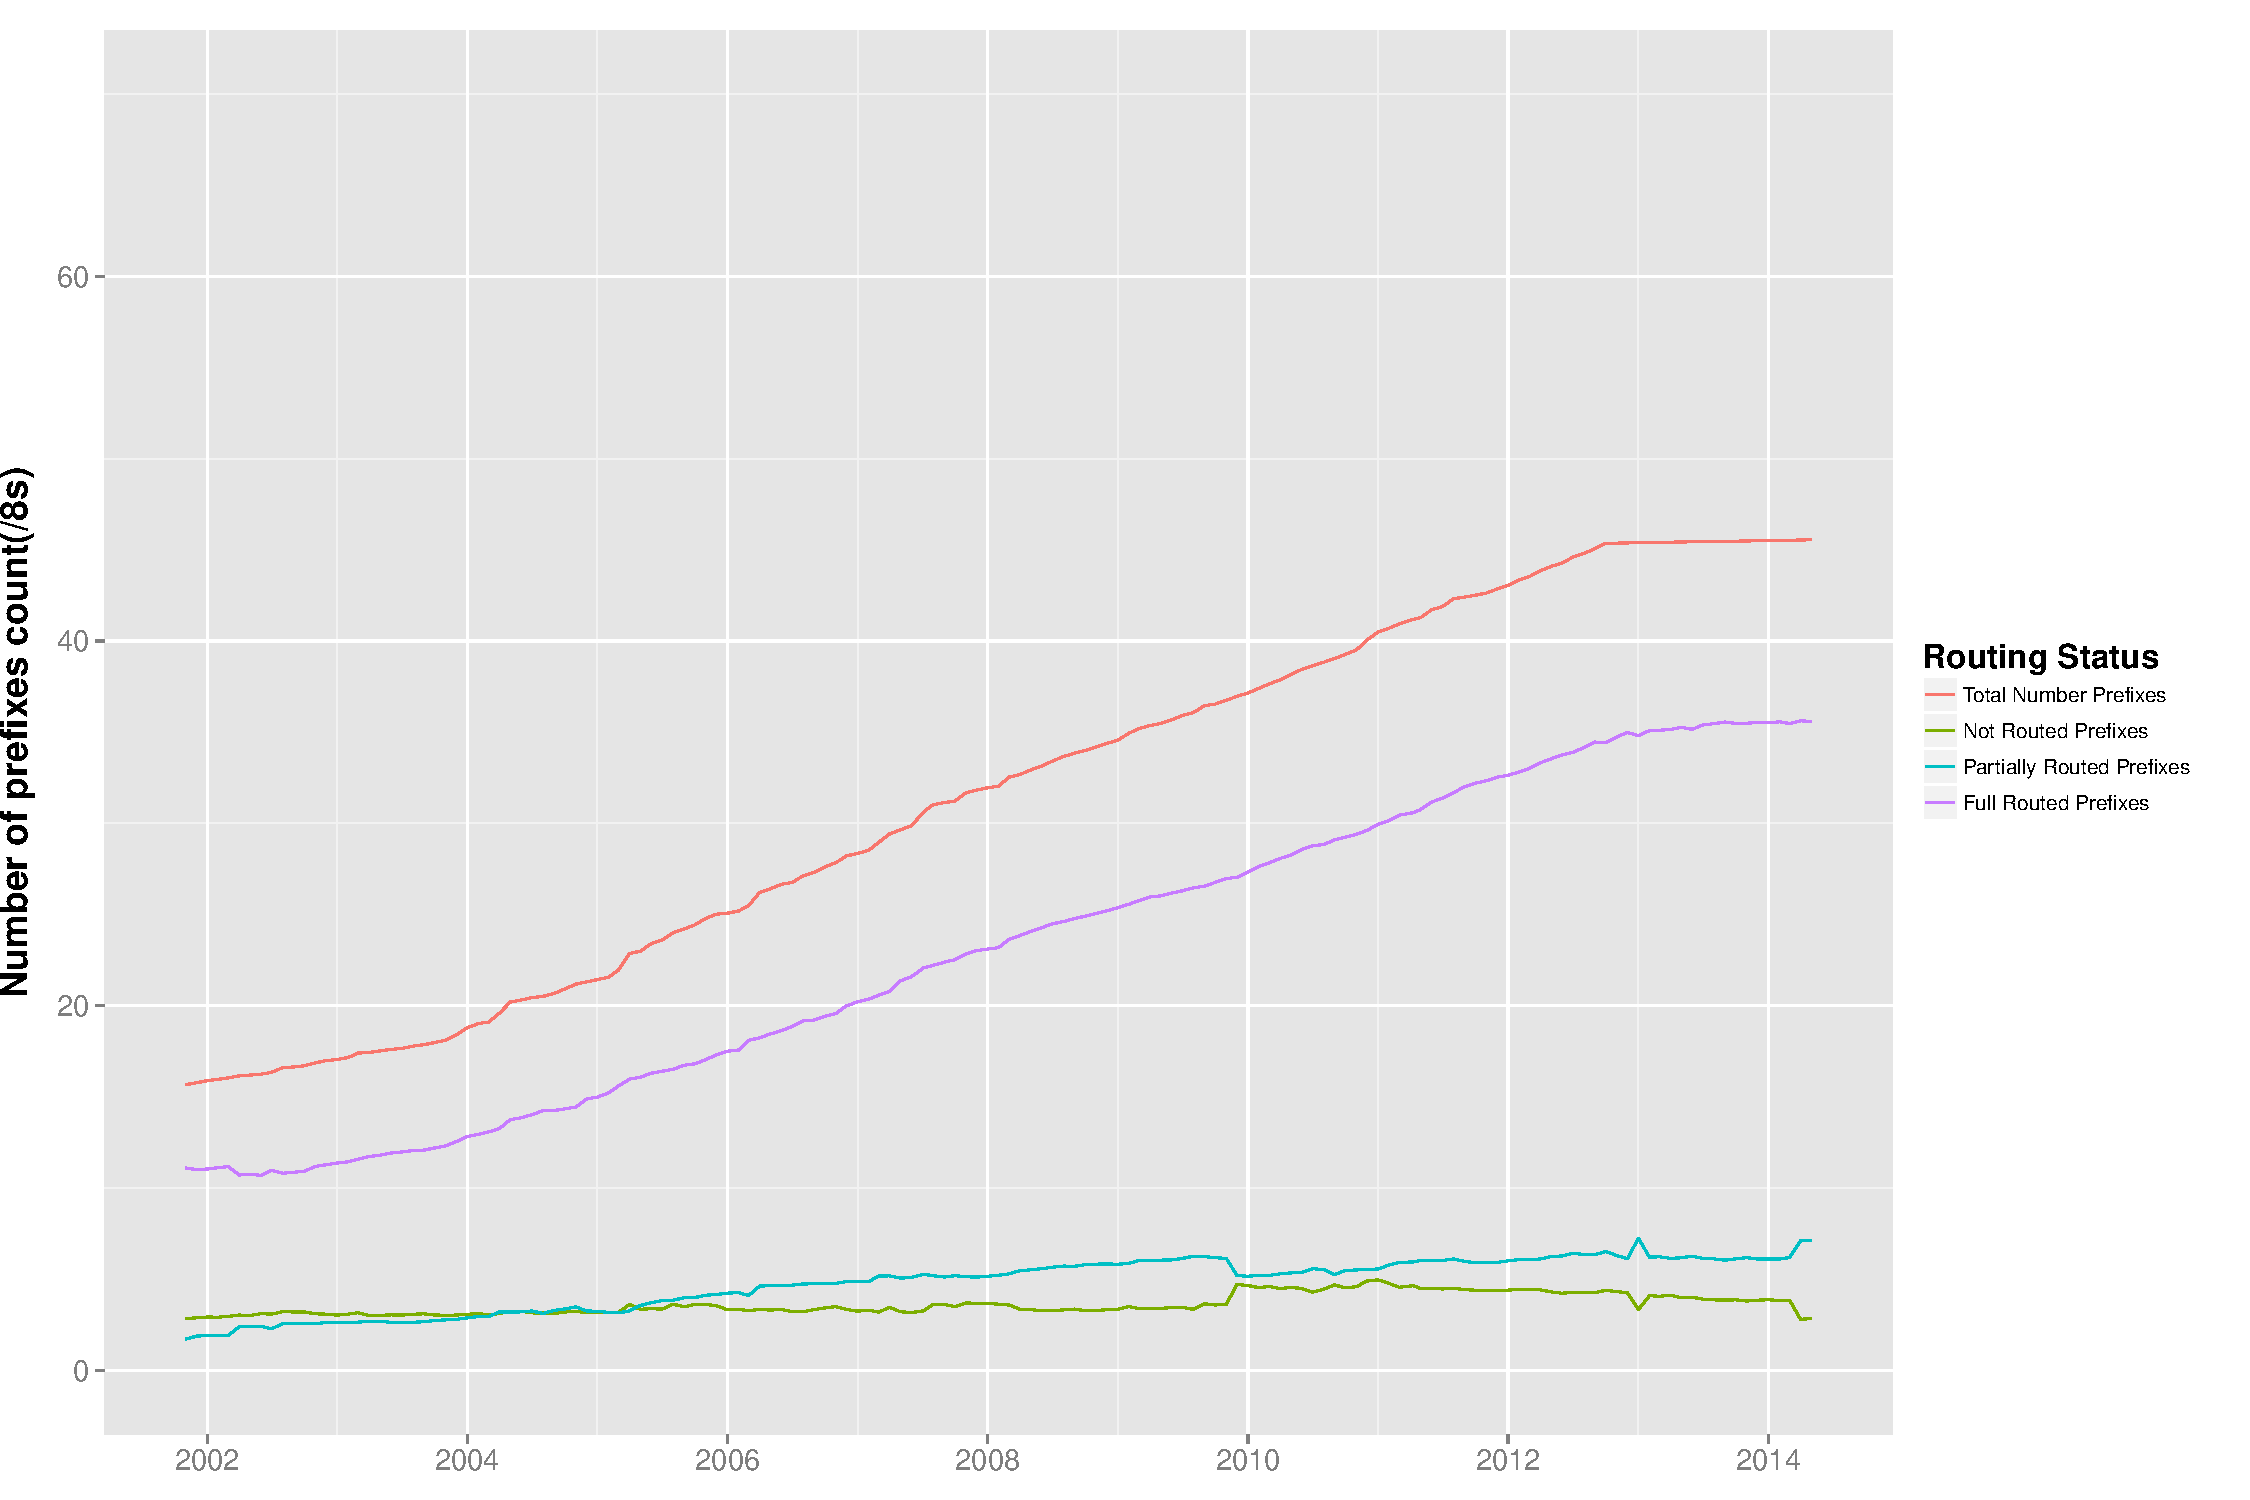
\includegraphics[scale=0.35]{routeStatusRipe8.pdf}
%\caption{Amount of address space of allocated prefixes, in RIPENCC, that is being %advertised in BGP in /8s, according to prefixes routing status}
%\label{fig:routingStatusRipe8}
%\end{figure}

Important is also to compare the routing status between the different RIRs. For that we normalize each one of the RIR values using the total number of prefixes count (/8s). The metric full routed prefixes is shown in Figure \ref{fig:routingStatusRelativeFull}.  

\begin{figure}[!h]
\centering
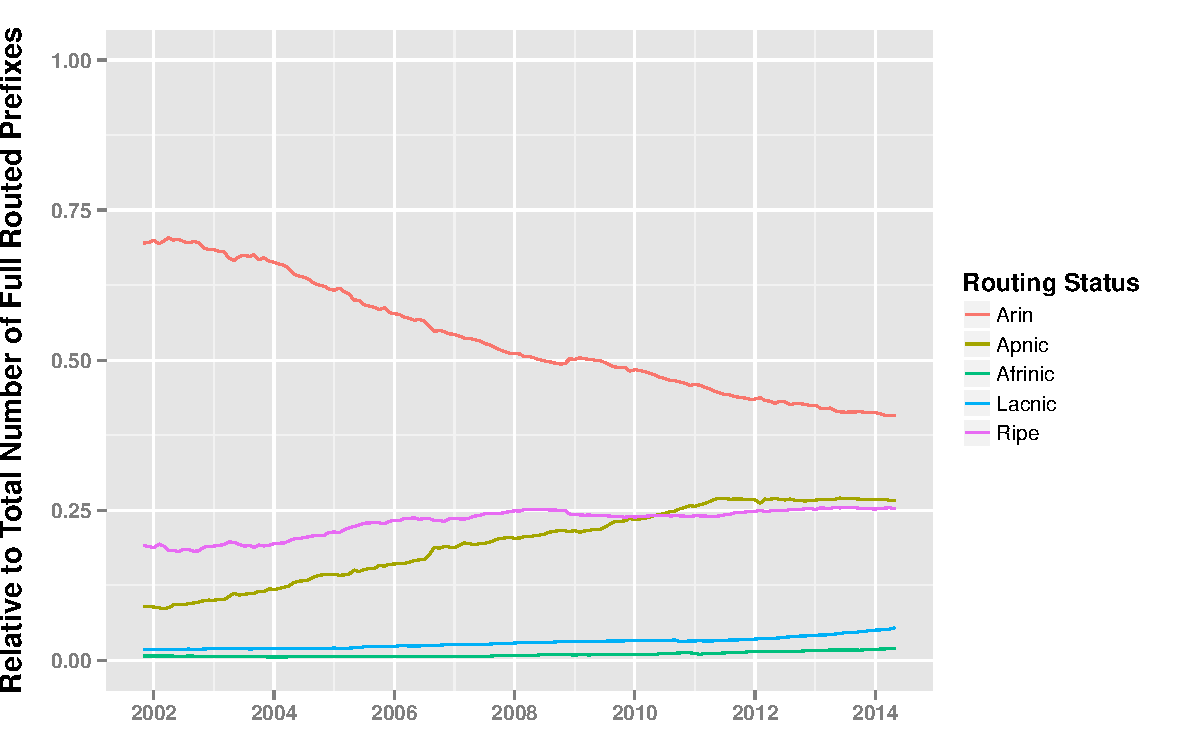
\includegraphics[scale=0.35]{routeStatusRelativeFull.pdf}
\caption{RIRs comparison of prefixes that are being fully routed}
\label{fig:routingStatusRelativeFull}
\end{figure}

We can see that ARIN has around 40\% of the entire routing address space that is fully routed. Then is RIPENCC and APNIC with around 25\% each, after LACNIC with around 7\% and last AFRINIC  with around 3\%.  
The next comparison was regarding the partially routed prefixes. It can be seen in Figure \ref{fig:routingStatusRelativePart}. 

\begin{figure}[!h]
\centering
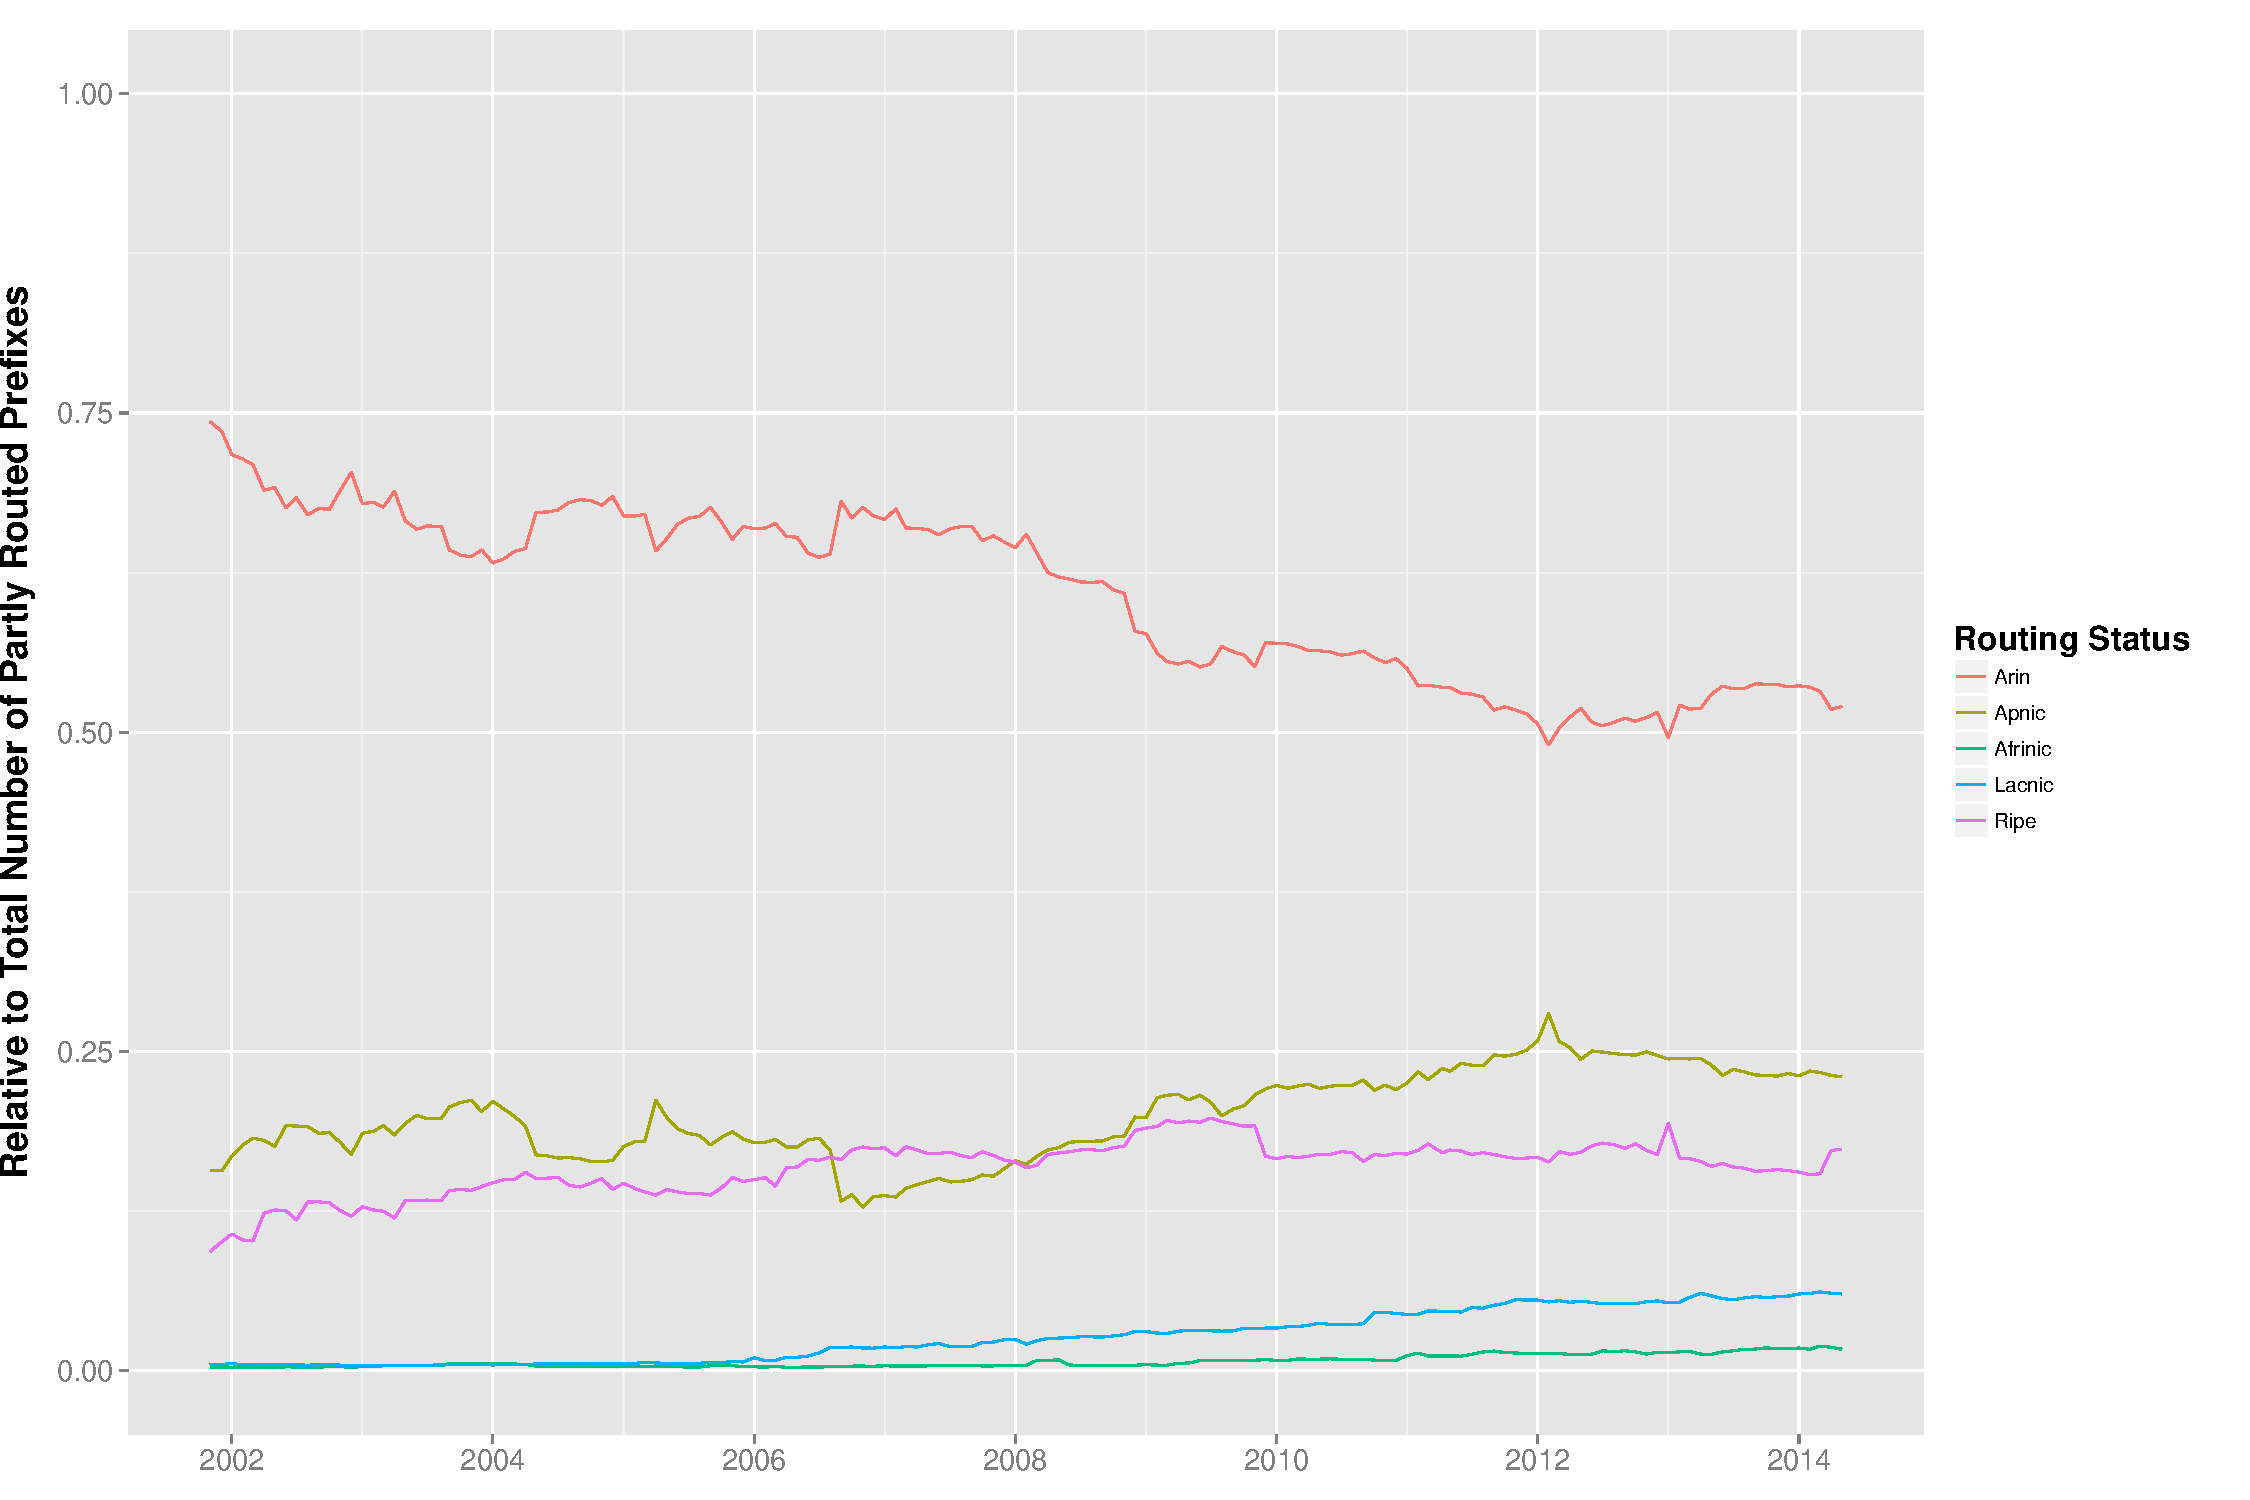
\includegraphics[scale=0.35]{routeStatusRelativePart.pdf}
\caption{RIRs comparison of prefixes that are being partially routed}
\label{fig:routingStatusRelativePart}
\end{figure}

We can see that ARIN has around 50\% of the entire routing address space that is fully routed. Then is APNIC with 25\%, RIPENCC with around 15\%, after LACNIC with around 7\% and last AFRINIC  with around 3\%. 
\clearpage

Regarding the metric not routed prefixes, the results are shown in Figure \ref{fig:routingStatusRelativeNot}. 

\begin{figure}[!h]
\centering
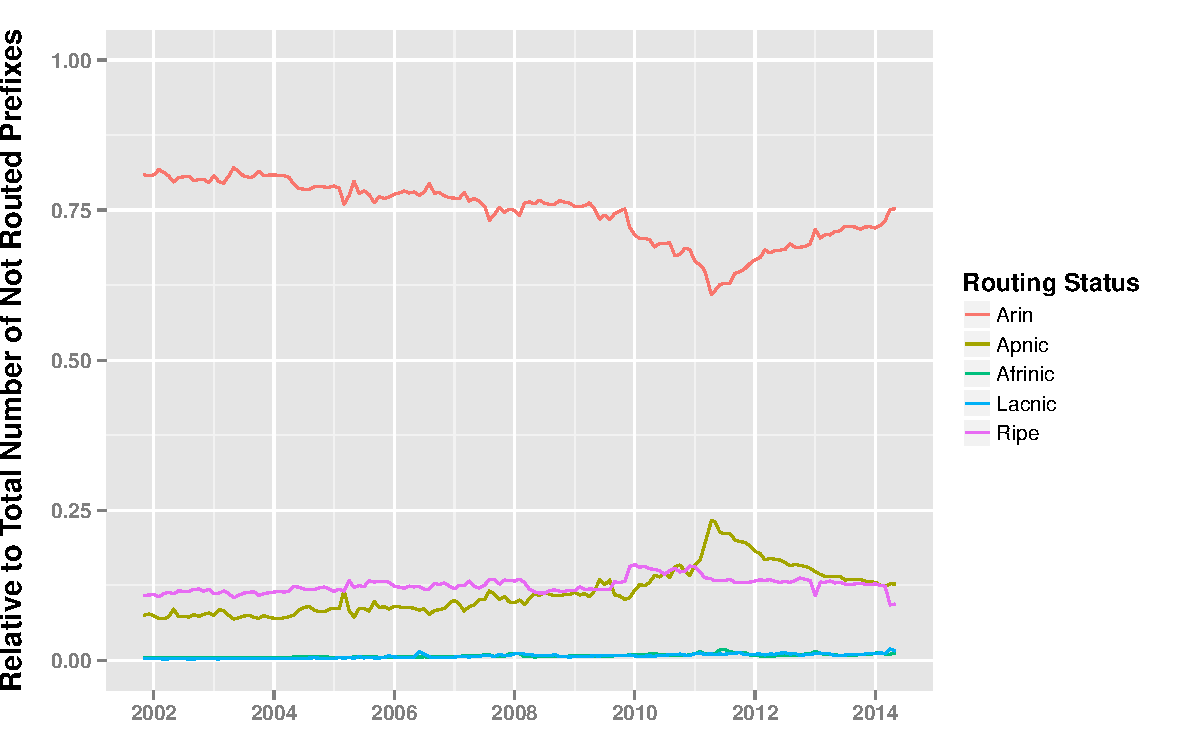
\includegraphics[scale=0.35]{routeStatusRelativeNot.pdf}
\caption{RIRs comparison of prefixes that are not being routed}
\label{fig:routingStatusRelativeNot}
\end{figure}

We can see that ARIN has around 75\% of the entire routing address space that is fully routed. Then is APNIC with 12\%, RIPENCC with around 8\%, after LACNIC with around 3\% and last AFRINIC  with around 2\%.


In Figure \ref{fig:heatmapLegacy} we can see a heatmap showing the mumber of /24s that are being advertised for each /8. In the y-axis it is shown the date and in the x-axis are shown /8 prefixes, such as 3.0.0.0, 4.0.0.0 and so on. We divided the prefixes into two categories "Legacy" and "Allocated" and created one Figure for each one. The division of the prefixes was done according to \cite{IANA_Address_Space}. Each date and prefix intersection shows the number of /24s being advertised in a log scale. We can see that more than half of these prefixes were already being routed in 2002 and maintained this trend accross the time period and show an increase in the number of /24s being advertised. On the other hand there are a significant number of prefixes that show no /24 being advertised during the whole time period. This prefixes are interesting, because when facing IPv4 address exhaustion, we notice quite a significant address space not being advertised. To be noted that although these prefixes are not advertised doesn't mean their are not used, but could be helpful to understand their situation.  

\begin{figure}[!h]
\centering
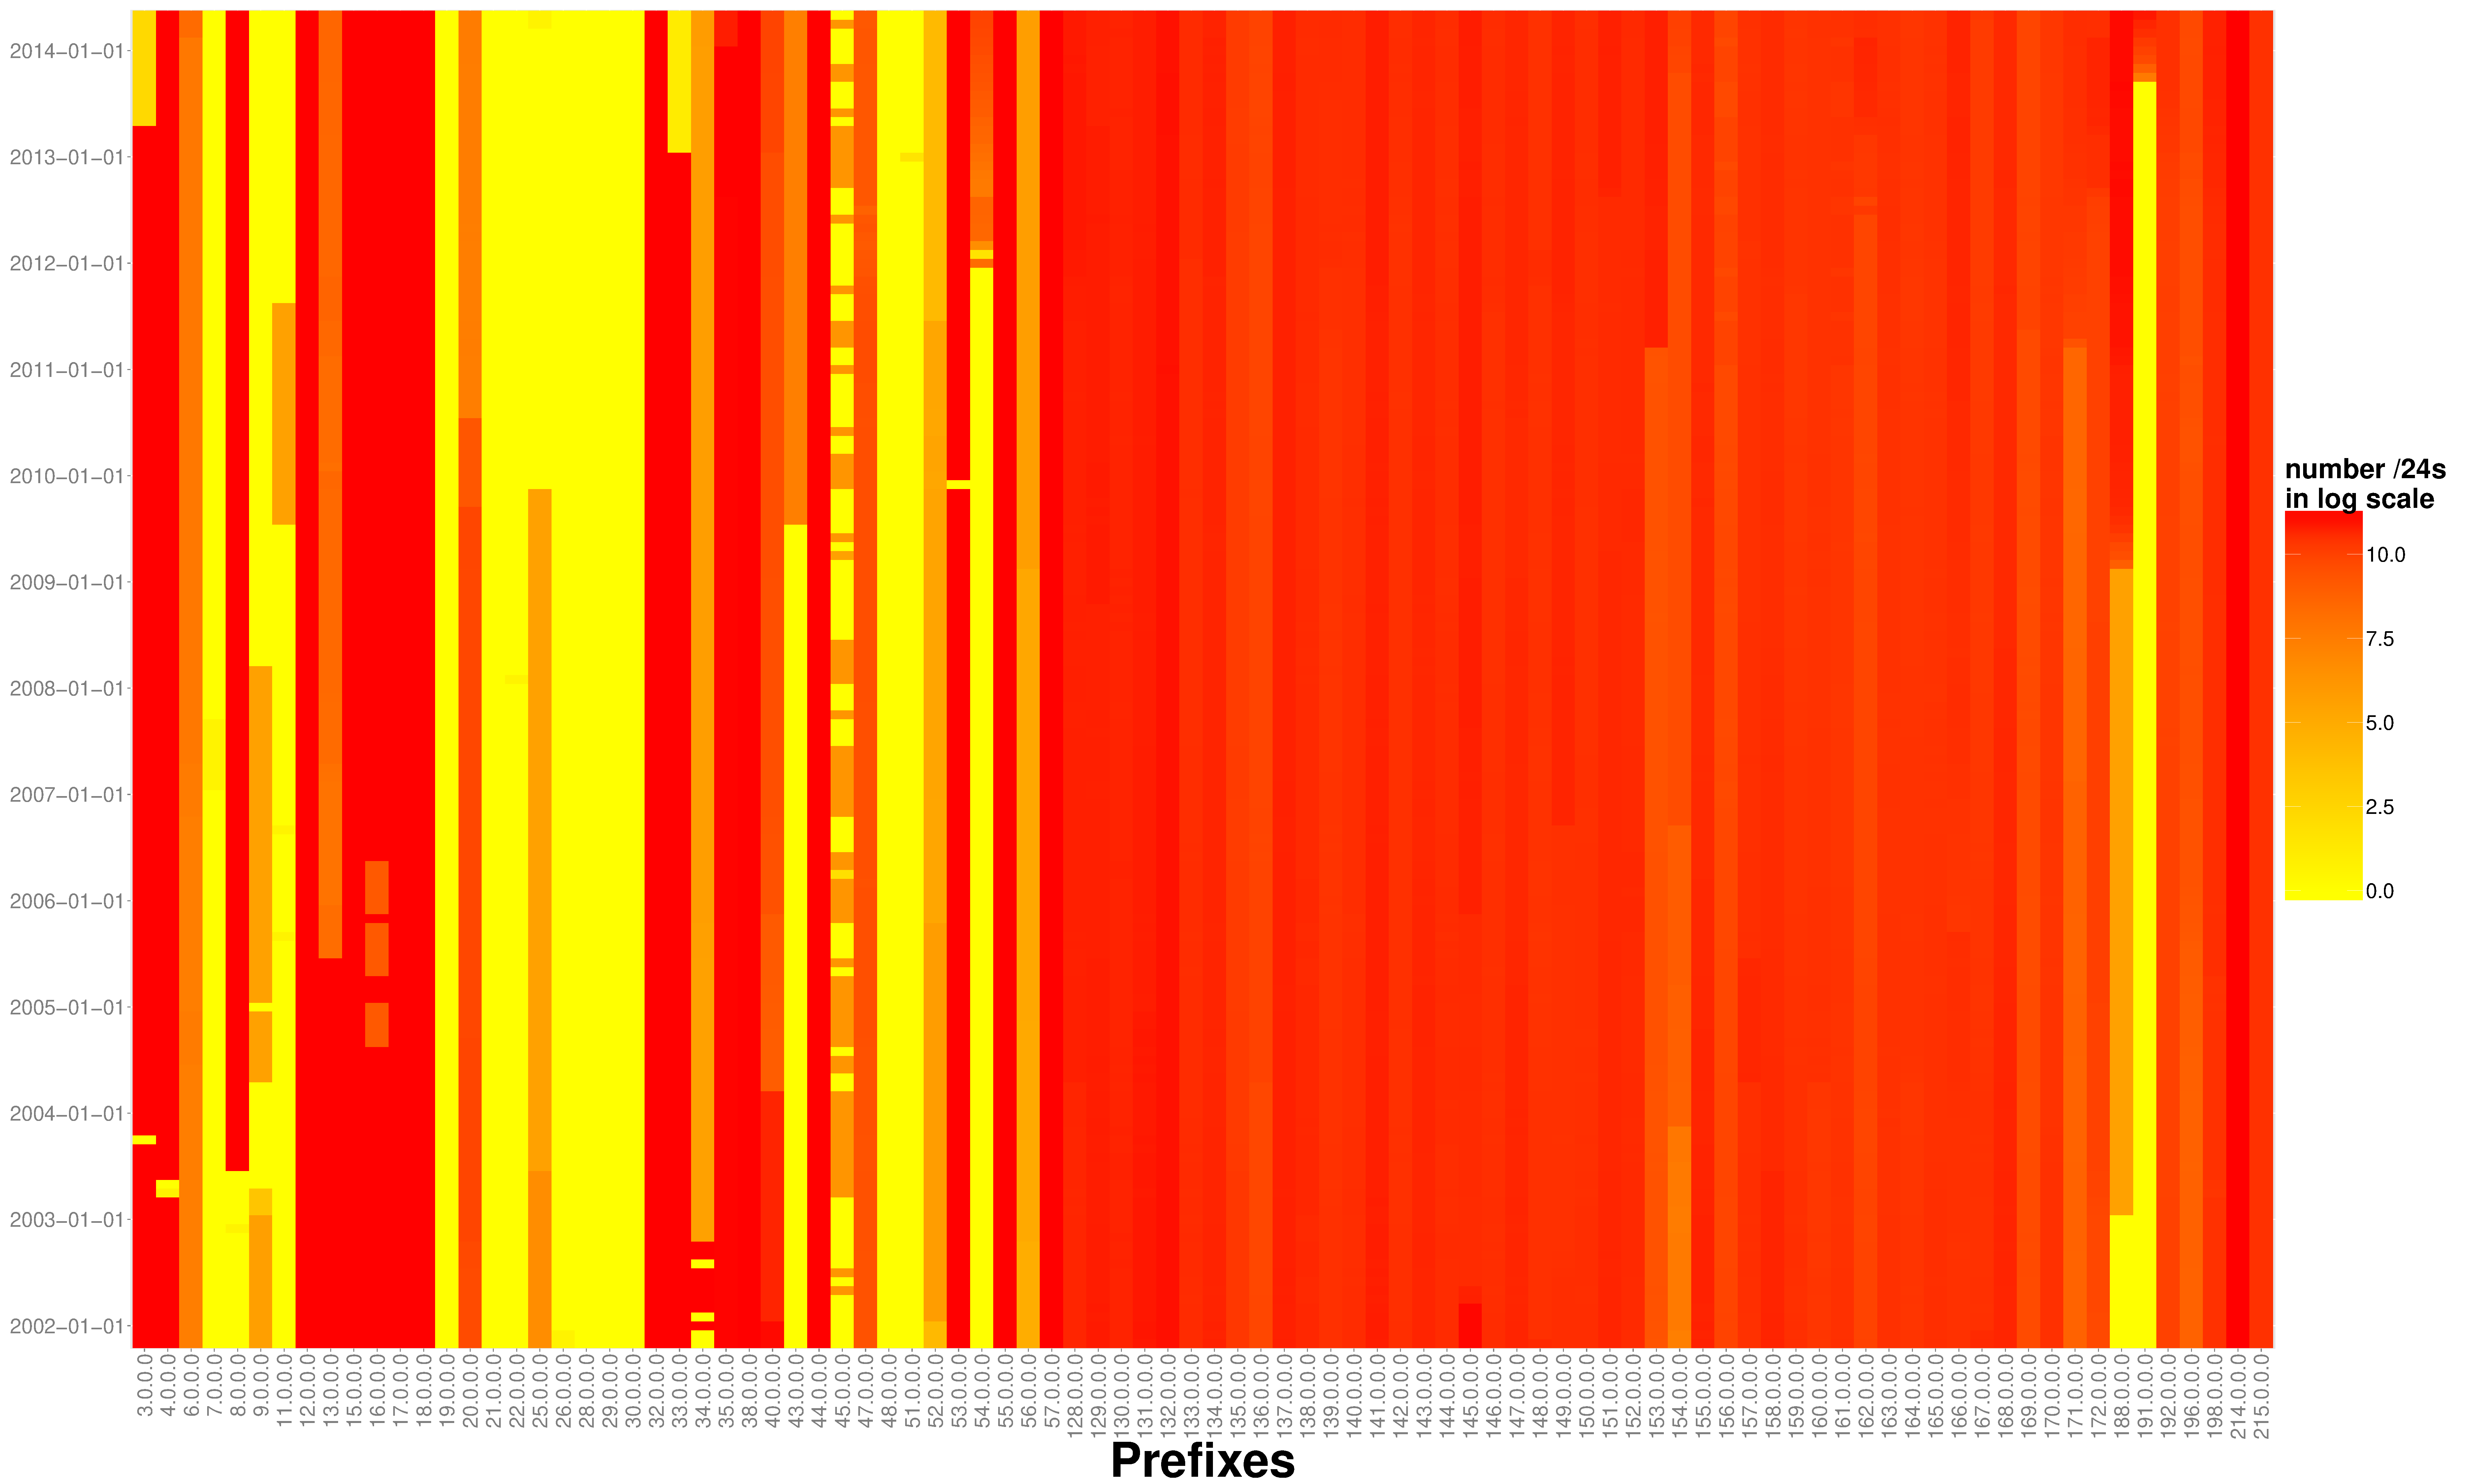
\includegraphics[scale=0.1]{heatmapLegacy.pdf}
\caption{Heatmap showing number of /24s being advertised by each /8 "Legacy" prefix}
\label{fig:heatmapLegacy}
\end{figure}

In Figure \ref{fig:heatmapAllocated} we show the results for the "Allocated" prefixes. Here we can see that most of the prefixes were not being advertised in 2002 and we can notice that as time progresses the prefixes start to be more and more advertised due to the allocations that are happening. We see that along the time more and more /24s are being advertised and when we have a closer look at 2011, IPv4 depletion date, we see that there are almost no prefixes available. Since 2011 we can notice the IPv4 exhaustion and that more and more addresses are being advertised.

\begin{figure}[!h]
\centering
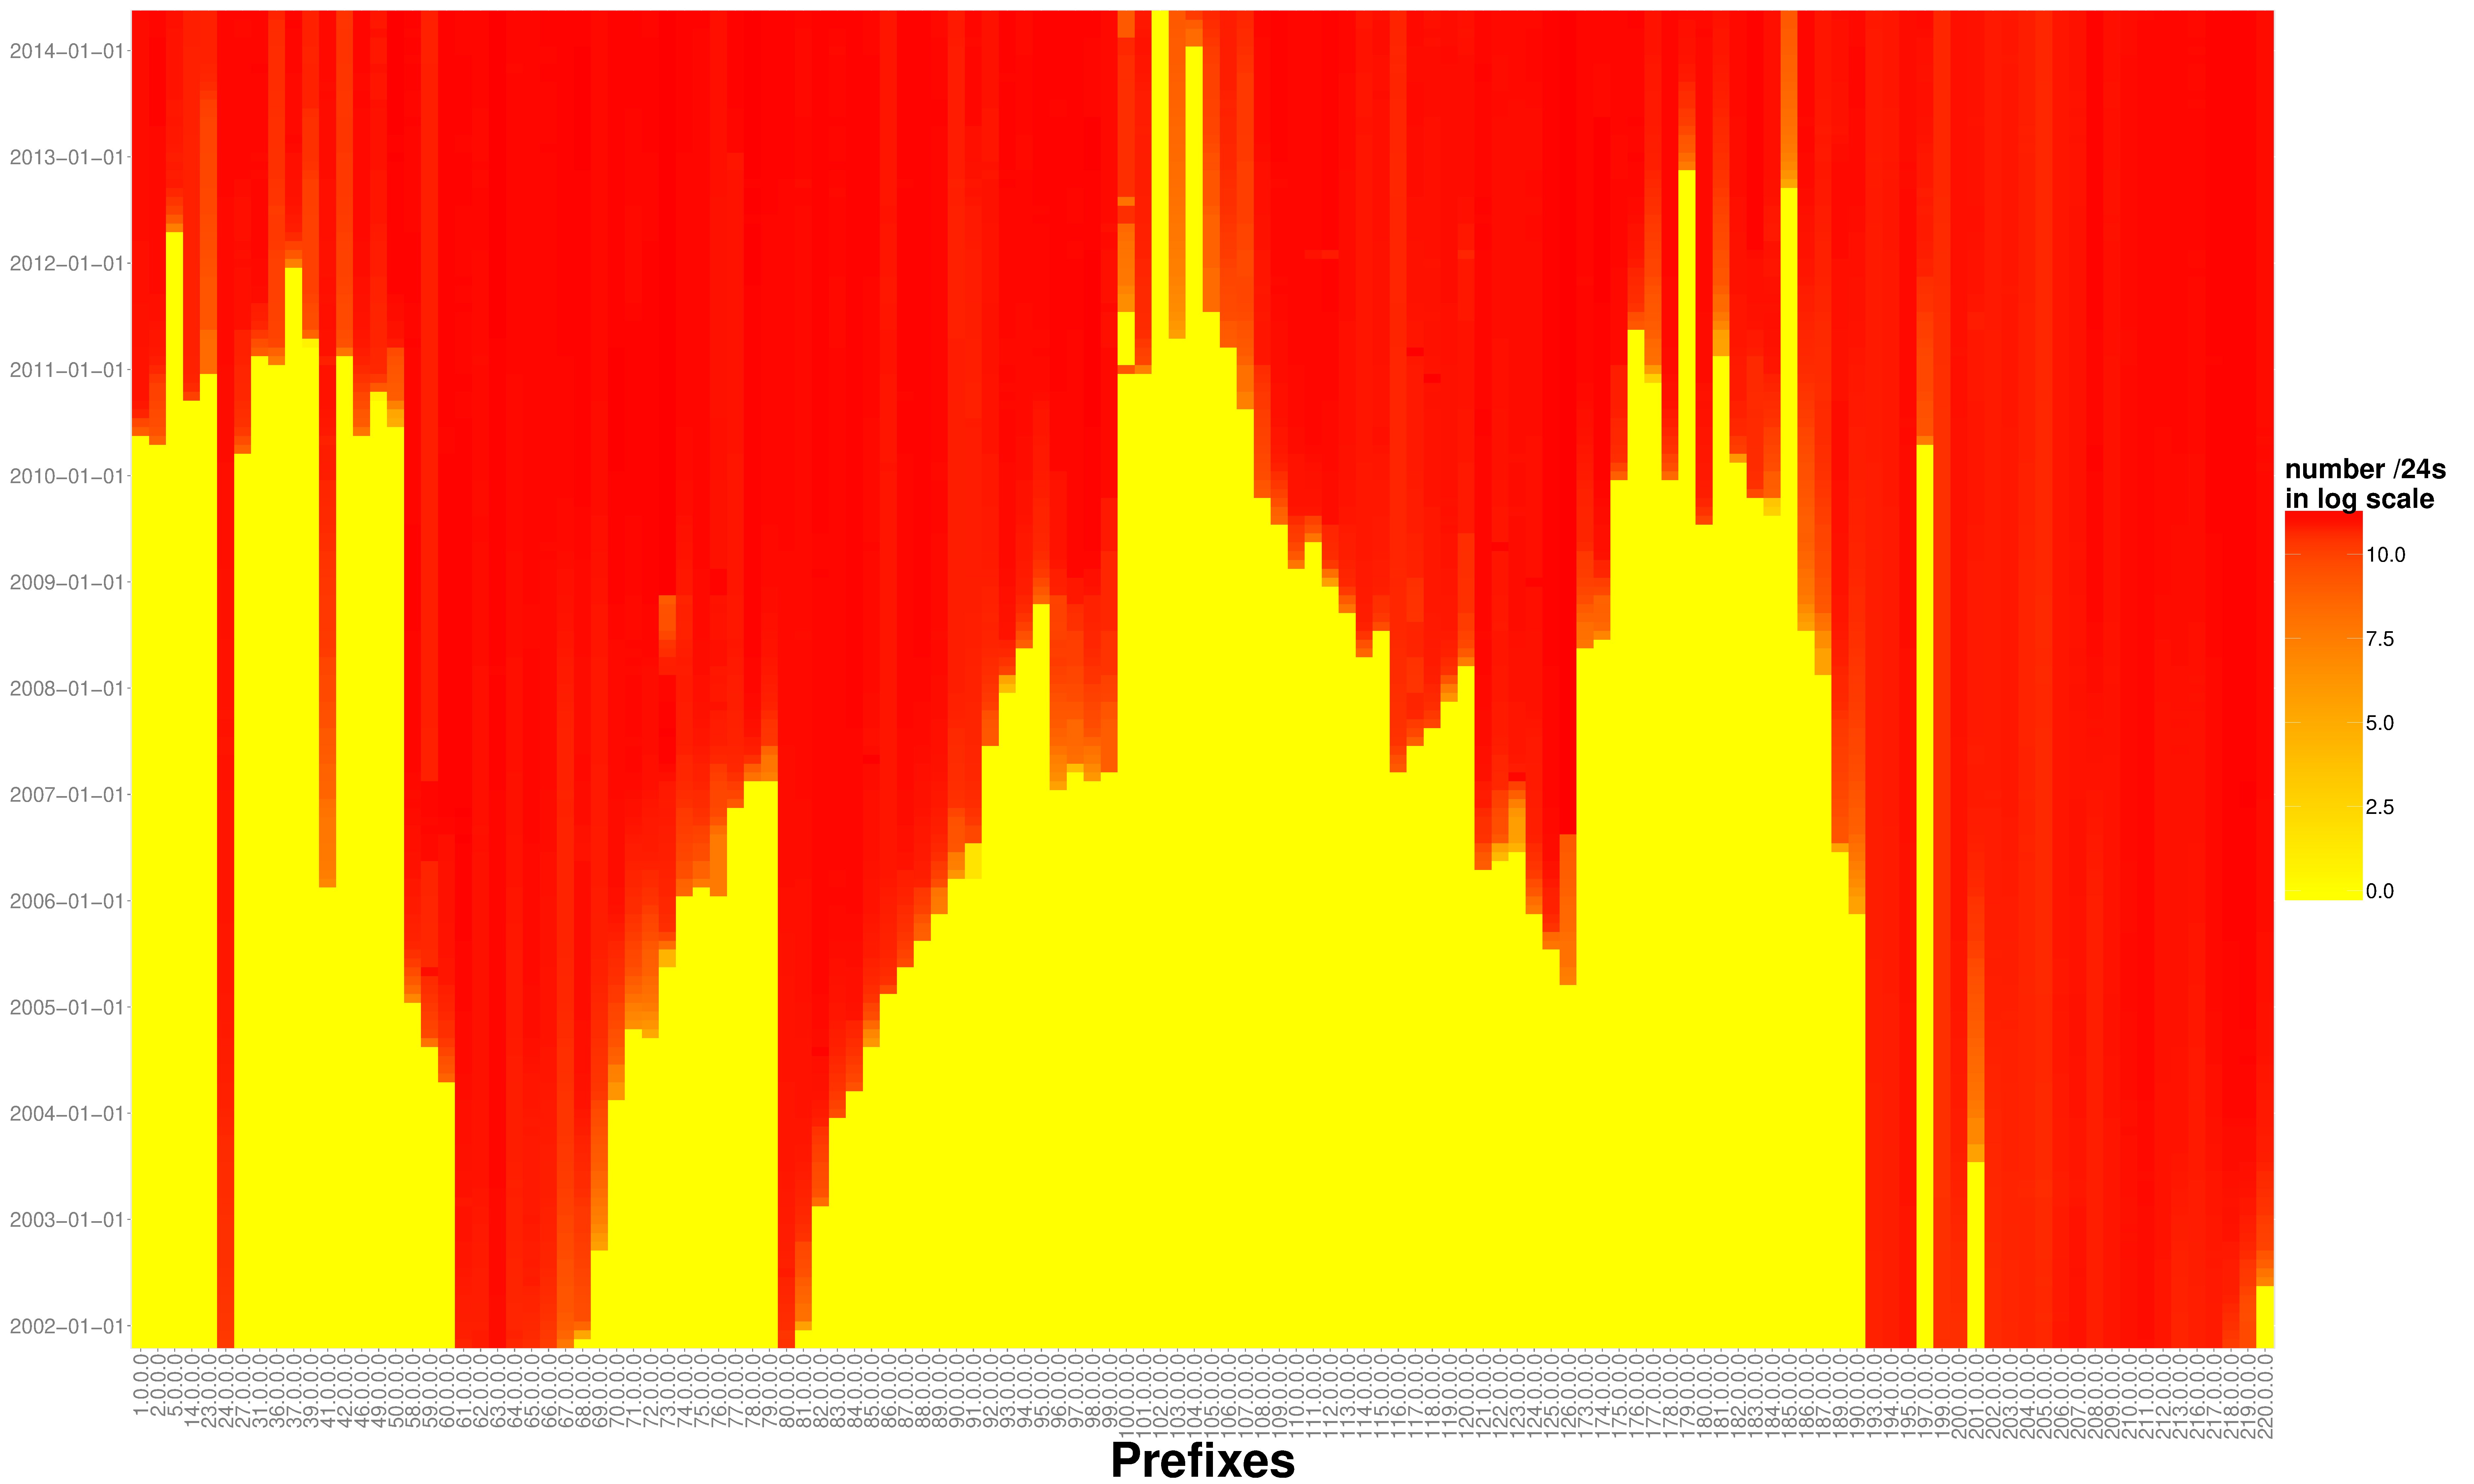
\includegraphics[scale=0.1]{heatmapAllocated.pdf}
\caption{Heatmap showing number of /24s being advertised by each /8 "Allocated" prefix}
\label{fig:heatmapAllocated}
\end{figure}


\begin{sidewaysfigure}[!h]

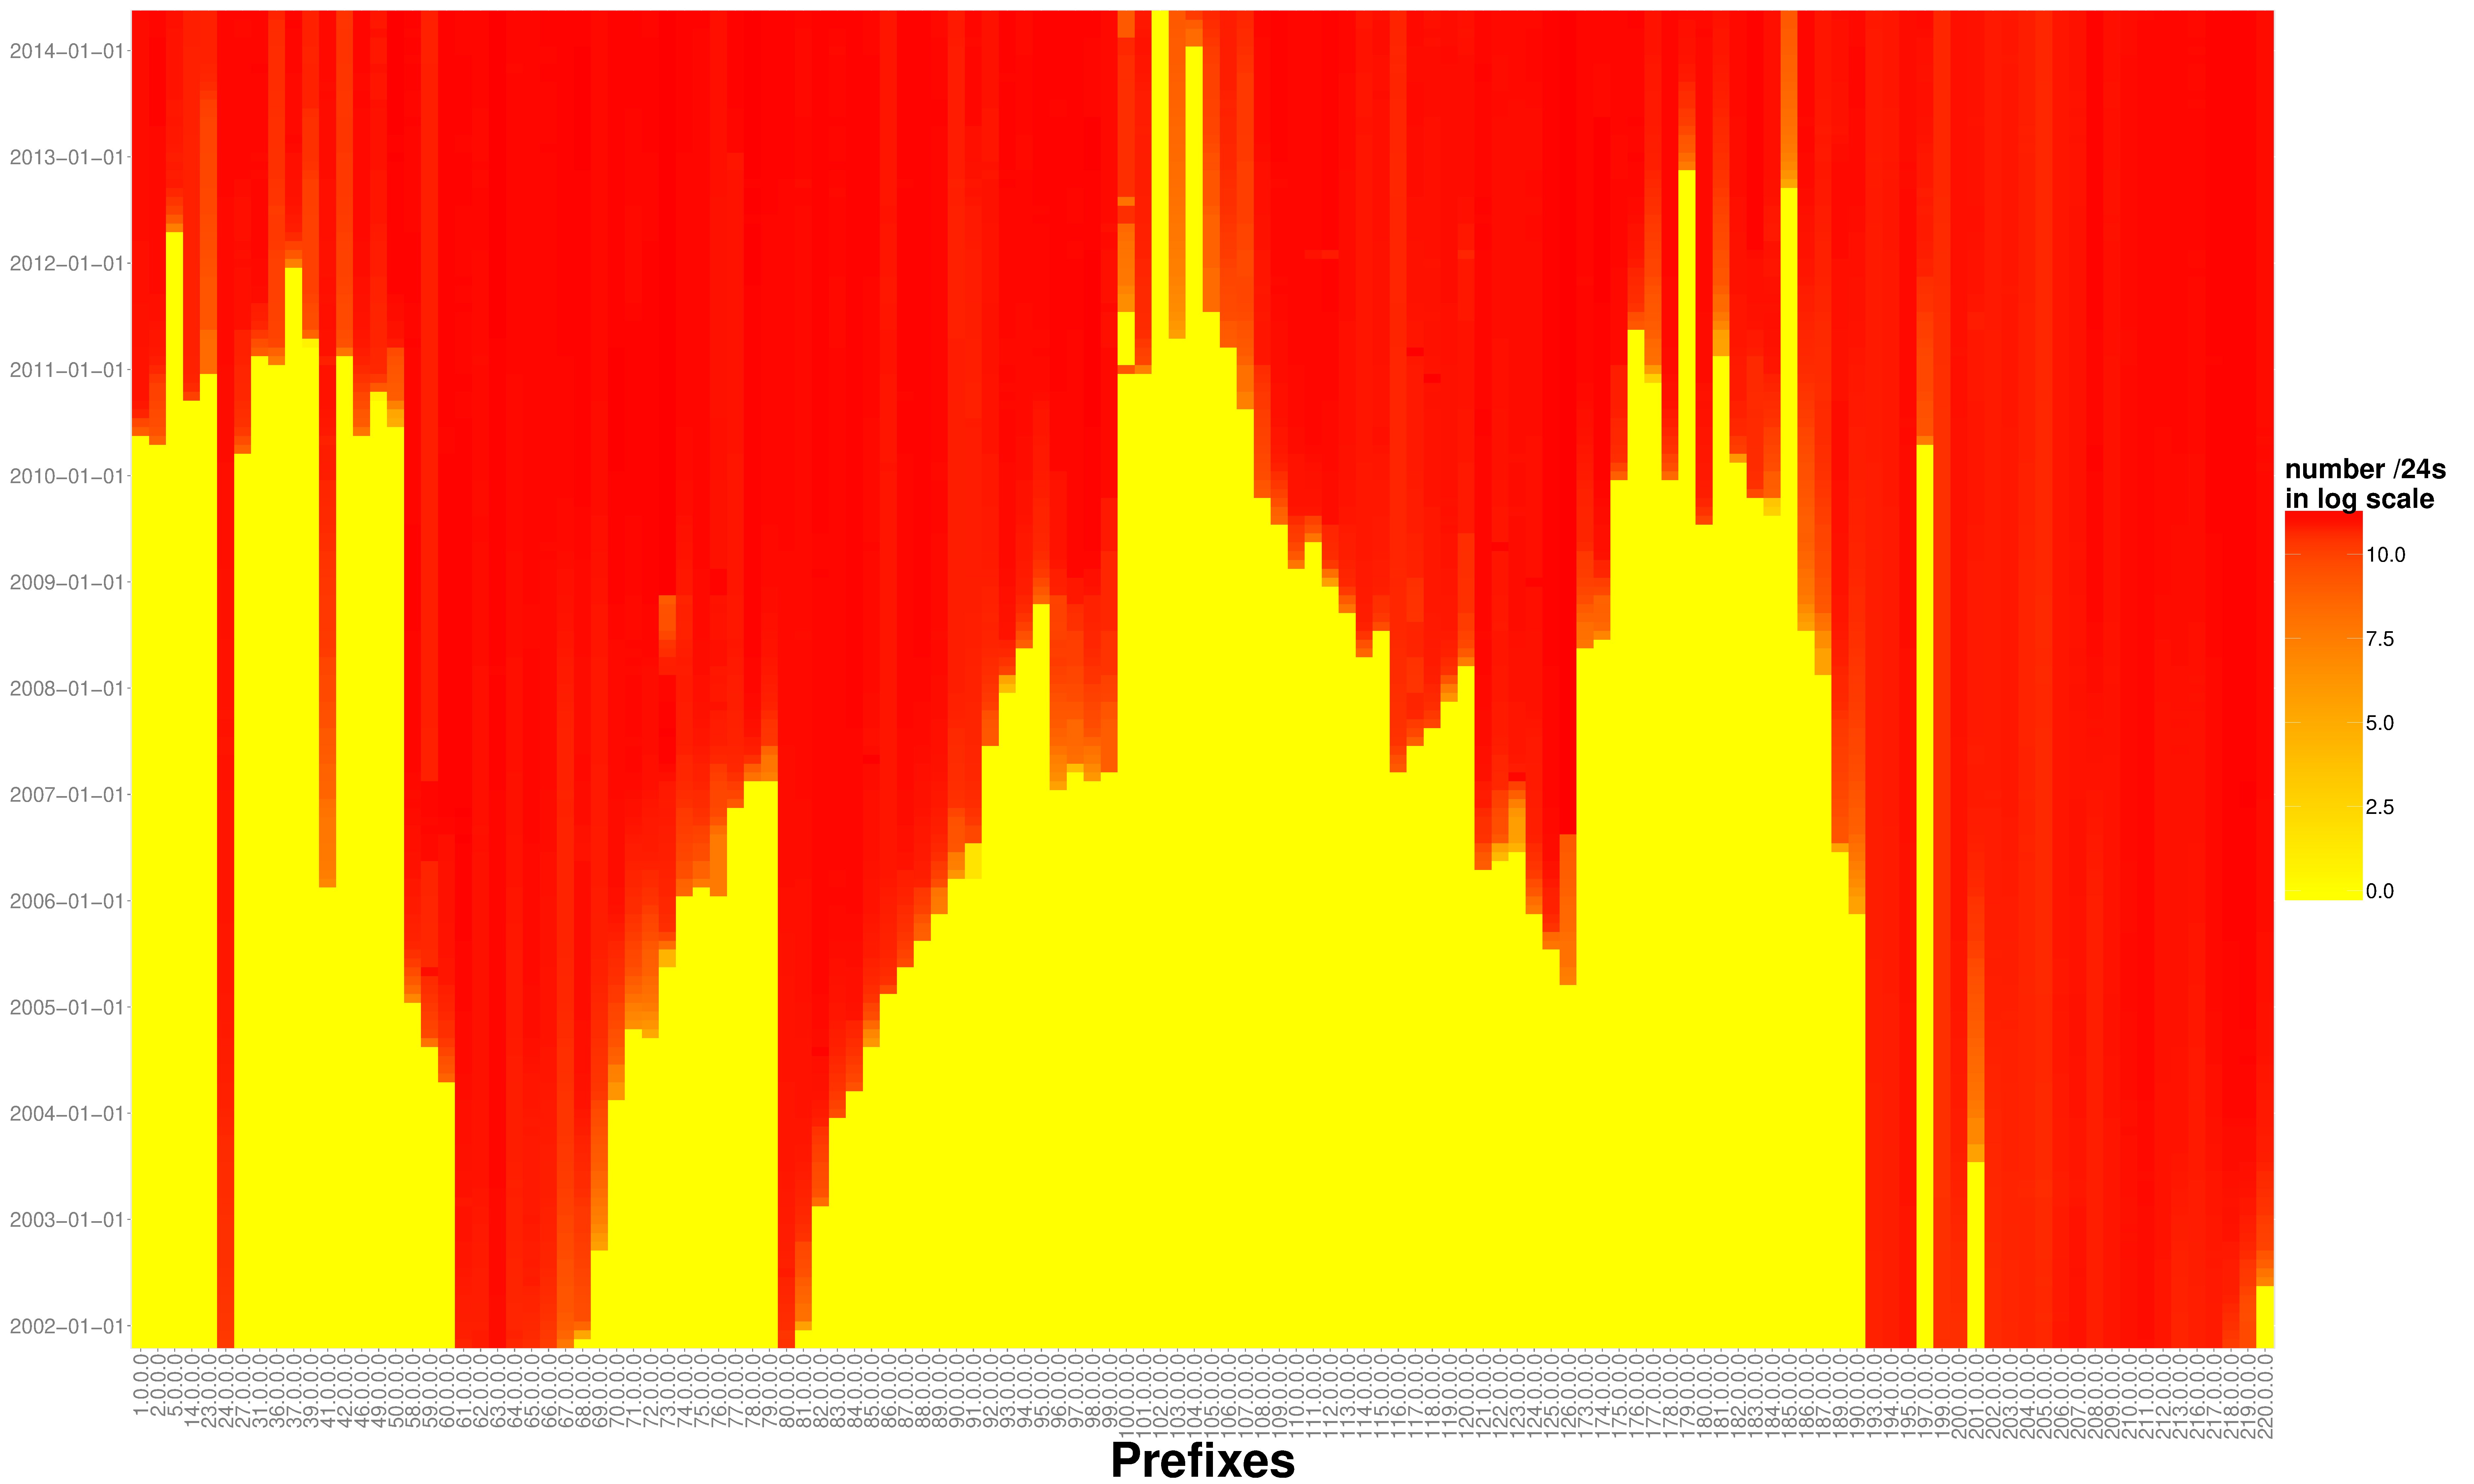
\includegraphics[scale=0.15]{heatmapAllocated.pdf}
\caption{Heatmap showing number of /24s being advertised by each /8 "Allocated" prefix}
\label{fig:heatmapAllocatedSideWays}
\end{sidewaysfigure}


\subsection{Prefixes and Multiple Origin ASes}


Our next step was to identify prefixes that were being advertised by multiple ASes. We took all the prefixes that were allocated and considered to be advertised by multiple prefixes every prefix that would be advertised by more than one AS.
The results are show in Figure \ref{fig:multipleAsesGlobal}. In the Total Number of Prefixes are considered all the prefixes allocated until a certain point in time and that were seen in the BGP routing data.
 
\begin{figure}[!h]
\centering
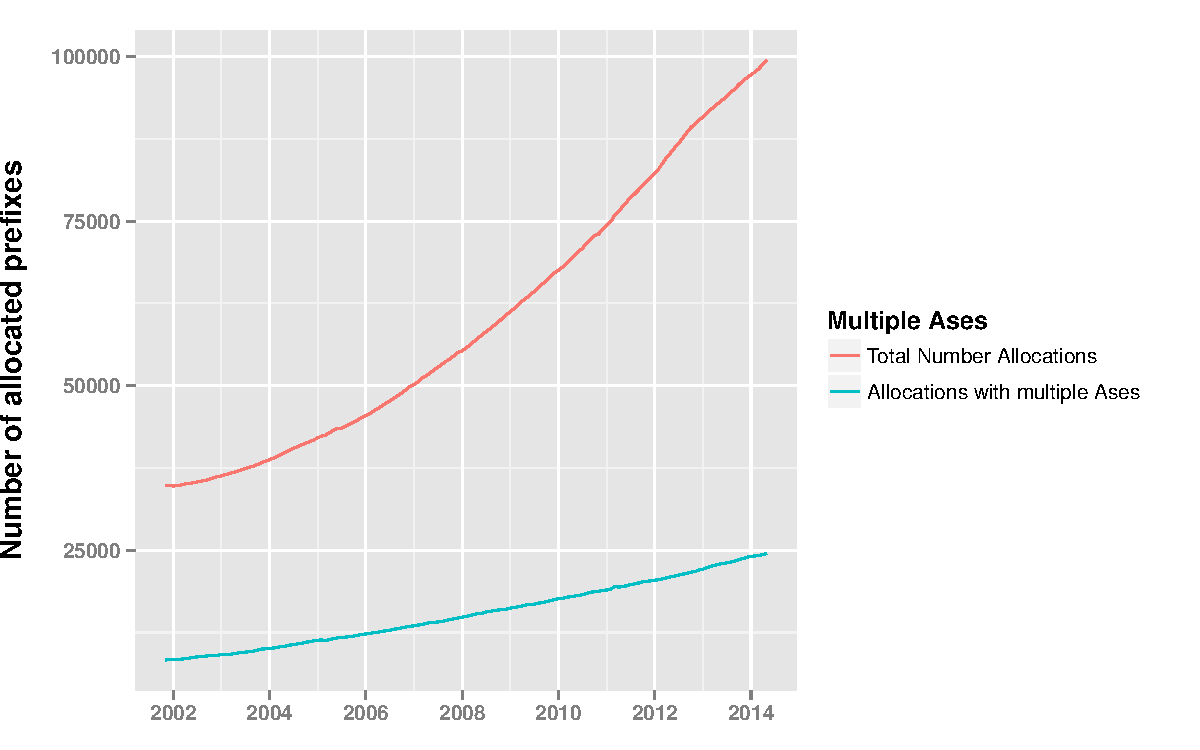
\includegraphics[scale=0.35]{multipleAsesGlobal.pdf}
\caption{Observed number of allocated prefixes being advertised by more than one AS}
\label{fig:multipleAsesGlobal}
\end{figure}

We can see that the total number of prefixes increases faster than the number of prefixes with multiple ASes. This shows that the majority of allocated prefixes are advertised by just one AS and the growth of allocations has not been reflected in the same proportion in prefixes with multiple ASes. Nevertheless the number of prefixes with multiple ASes has been increasing and taking into account that in recent times, since 2011, the blocks of addresses that were allocated were smaller and most probably are just advertised by just one AS, this can indicated that older blocks of prefixes are starting to be advertised by more than one AS. 
In Figure \ref{fig:multipleAsesOldGlobal} is shown the same plot, but just considering prefixes that were allocated before 1997.

\begin{figure}[!h]
\centering
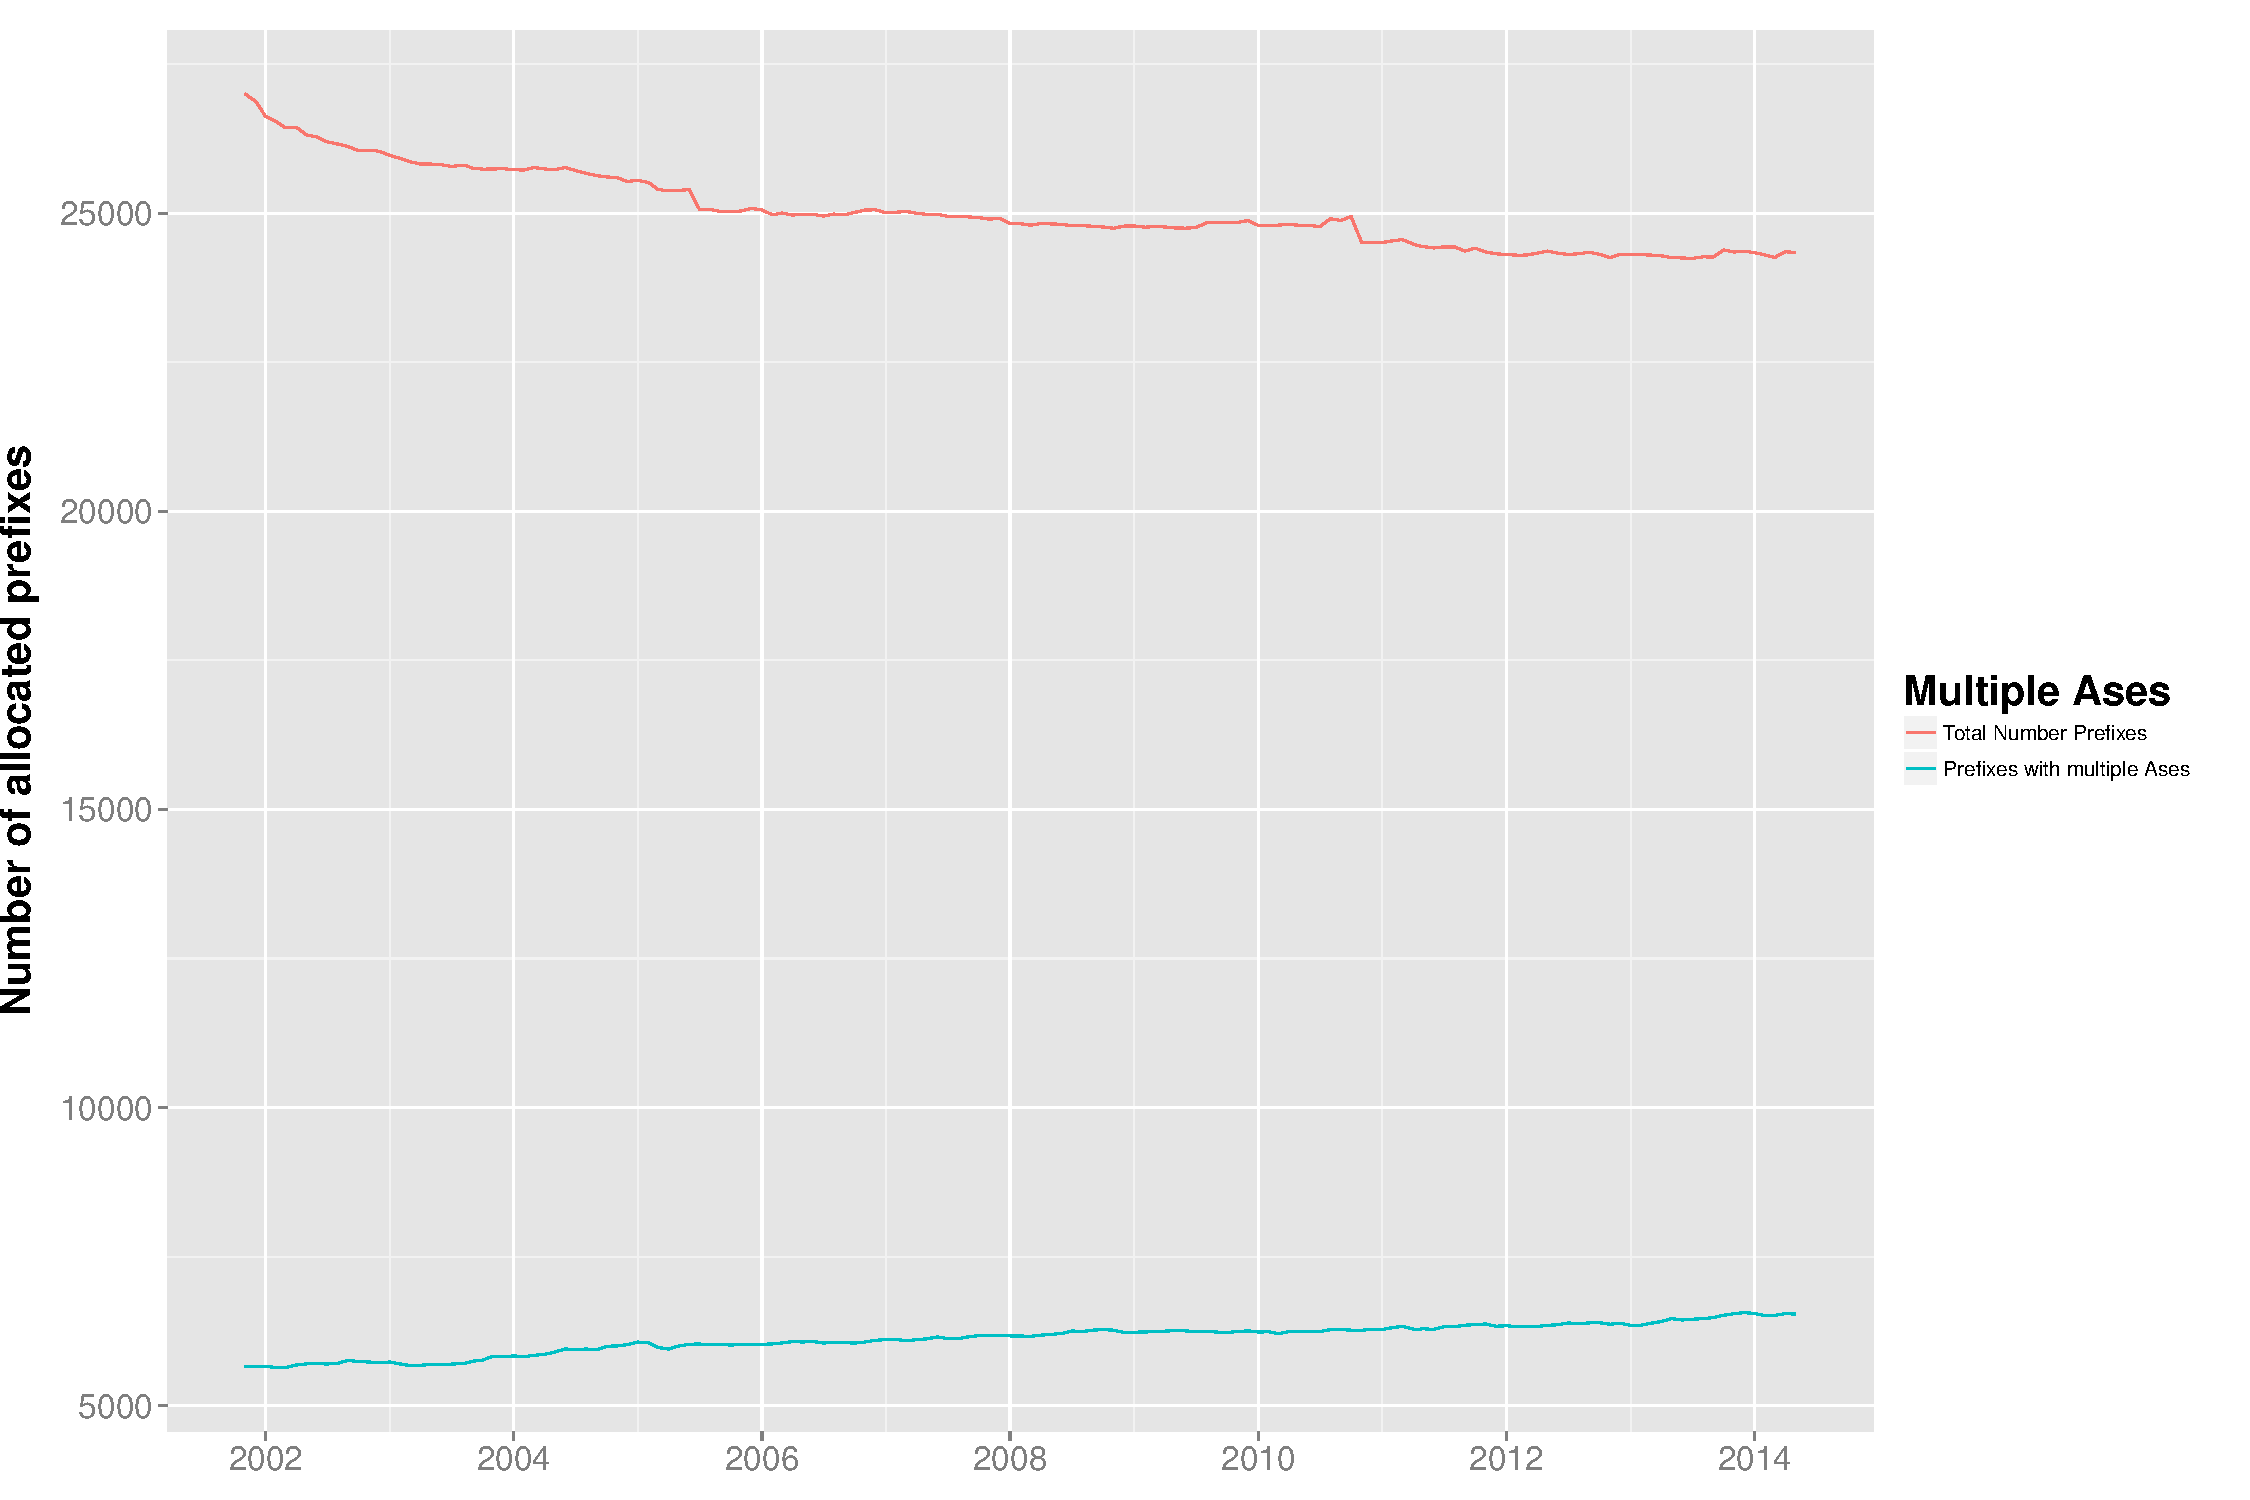
\includegraphics[scale=0.35]{multipleAsesOldGlobal.pdf}
\caption{Observed number of allocated prefixes, allocated before 1997, being advertised by more than one AS}
\label{fig:multipleAsesOldGlobal}
\end{figure}

We can see that, although there are less prefixes being advertised the number of prefixes with multiple ASes increases. Also we were not considering prefixes being allocated after 1997 and this growth on the number of prefixes with multiple ASes, althougth small, is significant and shows the address space is being shared by different ASes.
In Figure \ref{fig:multipleAsesNewGlobal} it is shown the plot for prefixes allocated after 1997.

\begin{figure}[!h]
\centering
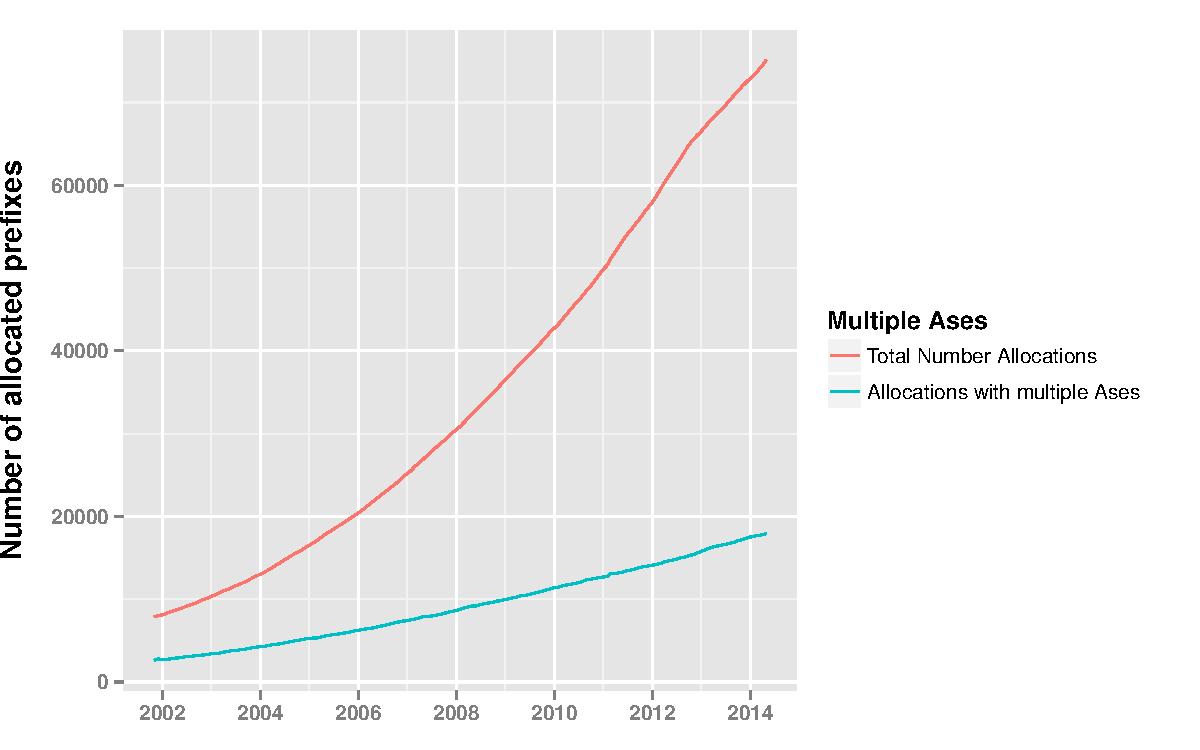
\includegraphics[scale=0.35]{multipleAsesNewGlobal.pdf}
\caption{Observed number of allocated prefixes, allocated after 1997, being advertised by more than one AS}
\label{fig:multipleAsesNewGlobal}
\end{figure}

We can see that the total number of prefixes allocated increased at a high rate, as expected, and the number of prefixes being advertised by multiple ASes also increased but with a much slower rate. Regarding that from 2011 some RIRs changed their allocation policy and considering that from this change the ASes that required prefixes were the only ones advertising them, this increase in the number of prefixes with multiple ASes is significant.

In Figure \ref{fig:heatmapLegacyMulti} we can see a heatmap showing the mumber of ASes that are advertising for each /8. In the y-axis it is shown the date and in the x-axis are shown /8 prefixes, such as 3.0.0.0, 4.0.0.0 and so on. We divided the prefixes into two categories "Legacy" and "Allocated" and created one Figure for each one. The division of the prefixes was done, once again, according to \cite{IANA_Address_Space}. Each date and prefix intersection shows the number of Ases that are advertising in a log scale. We can see that the majority of prefixes that were being advertised since the beggining of the time period, showed an increase in the number of ASes that are advertising subnet within the prefix.   

\begin{figure}[!h]
\centering
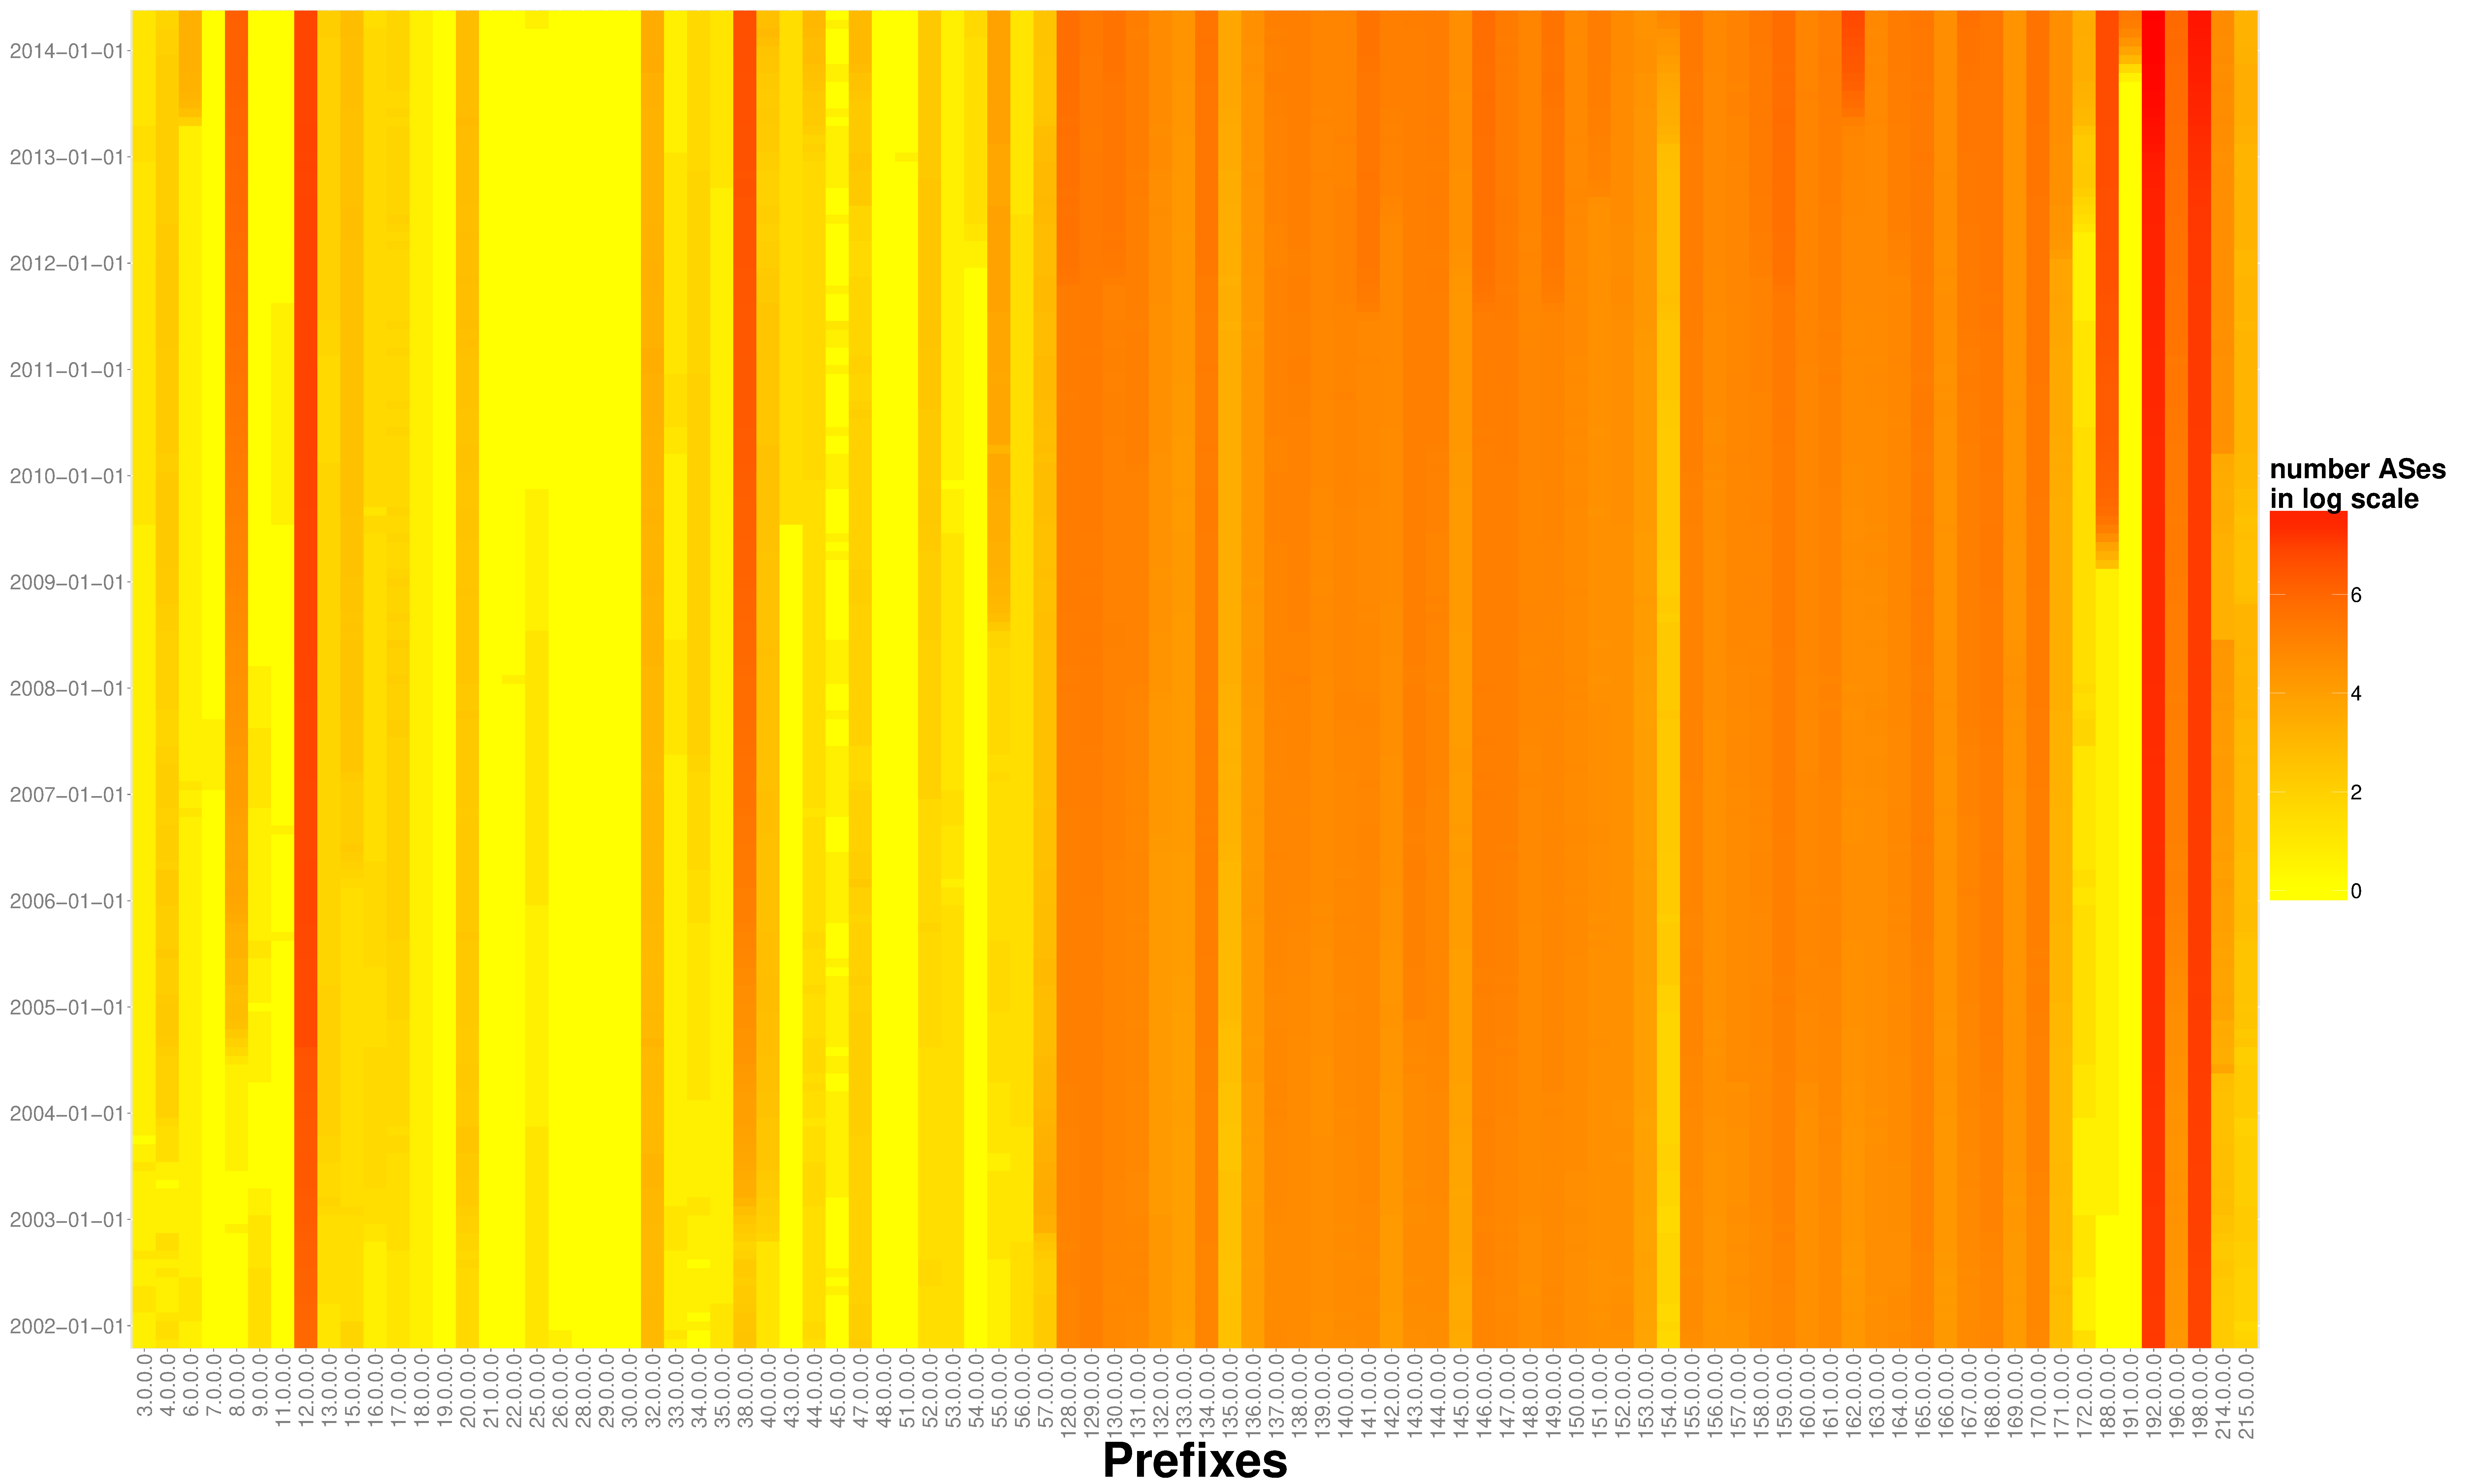
\includegraphics[scale=0.1]{heatmapLegacyMulti.pdf}
\caption{Heatmap showing number of ASes advertising prefixes for each /8 "Legacy" prefix}
\label{fig:heatmapLegacyMulti}
\end{figure}

In Figure \ref{fig:heatmapAllocatedMulti} we show the results for the "Allocated" prefixes. We can see, as expected, that the majority of the prefixes were not being advertised by any AS in 2002. As time progresses we notice that ASes start advertising for each of the prefixes and in 2011 most prefixes have already ASes advertising their subnets. Since then we notice and increase in the number of ASes advertising for each prefix.

\begin{figure}[!h]
\centering
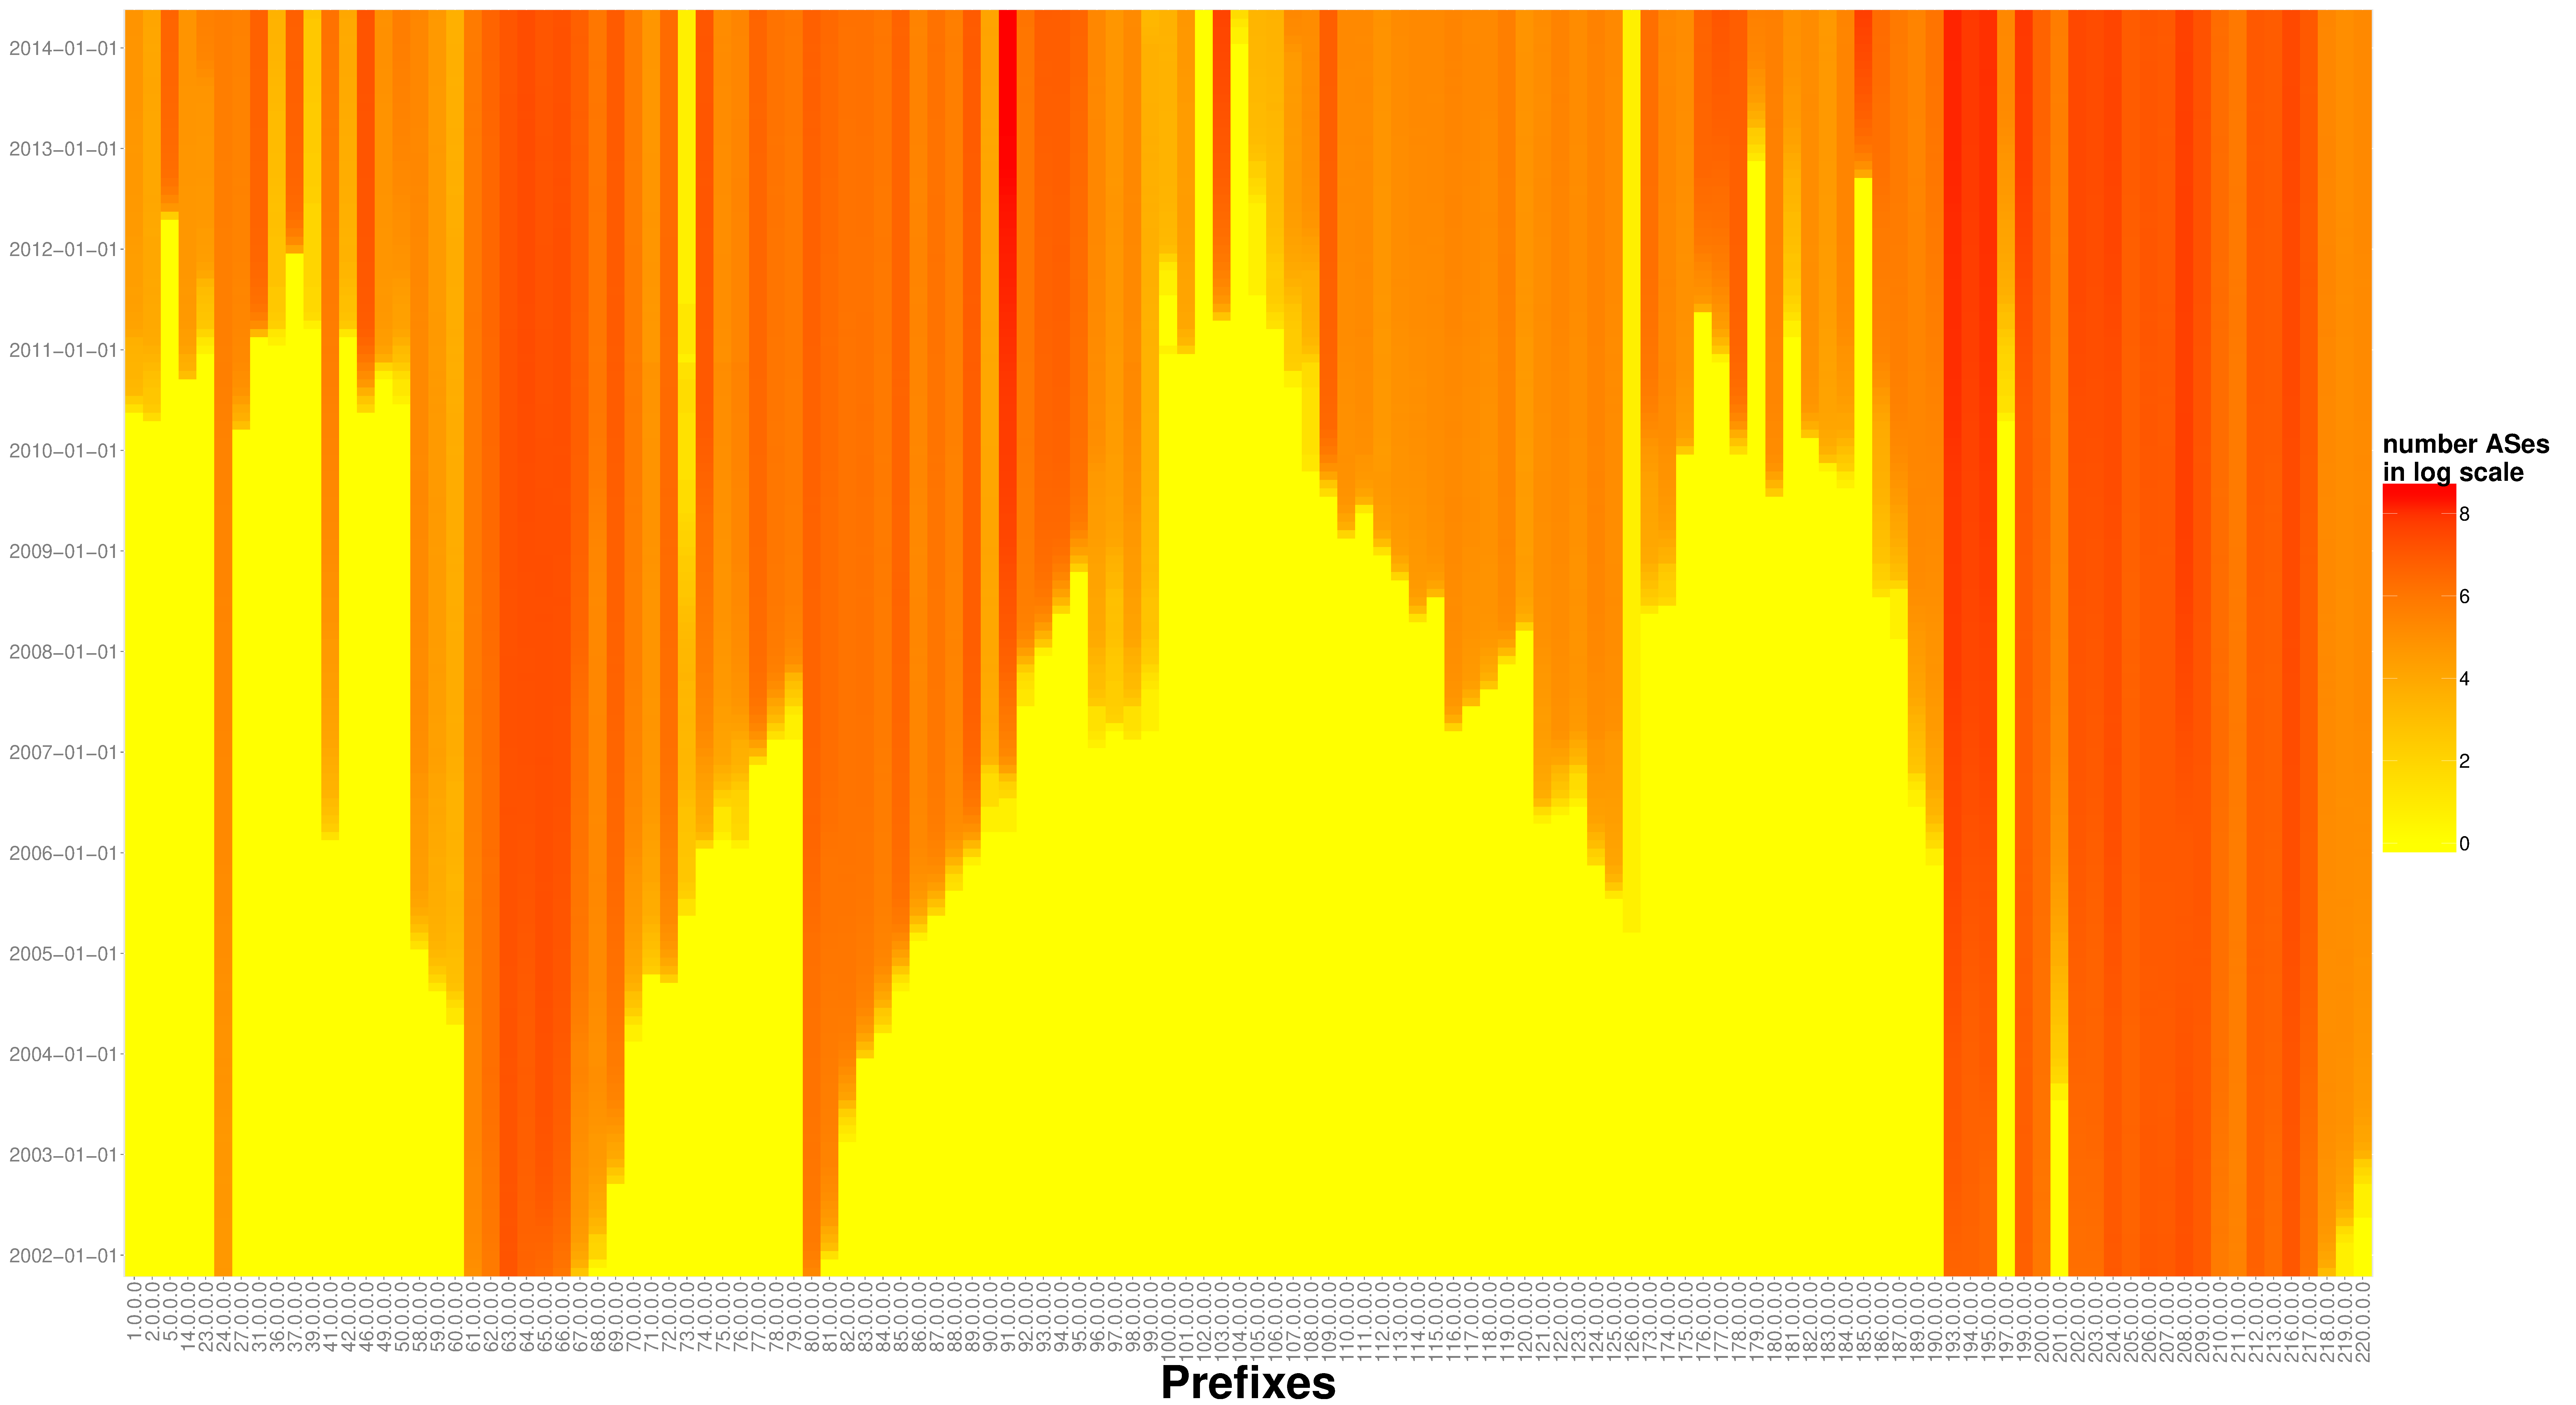
\includegraphics[scale=0.1]{heatmapAllocatedMulti.pdf}
\caption{Heatmap showing number of ASes advertising prefixes for each /8 "Allocated" prefix}
\label{fig:heatmapAllocatedMulti}
\end{figure}

\subsection{Multiple Origin ASes and IRR}

Our next step was to investigate what was happening with the old prefixes. Because the new ones were being allocated throughout the time it was expected to see them with an increasing number of ASes, but for old prefixes the behaviour could be different. 
In Figure \ref{fig:oldNetworks} we can see the ten allocated prefixes, allocated before 1997, that are being advertised by the highest number of ASes.

\begin{figure}[!h]
\centering
\includegraphics[scale=0.35]{oldNetworks.pdf}
\caption{Observed number of ASes for the ten prefixes being advertised by more addresses, allocated before 1997}
\label{fig:oldNetworks}
\end{figure}

From the Figure we decided to choose the prefixes 8.0.0.0, 12.0.0.0 and 38.0.0.0 for further observation. Using whois we found out that 8.0.0.0 is registered to Level 3 Communications, 12.0.0.0 is registered to AT\&T Services and 38.0.0.0 to PSINet, which was acquire by Cogent Communications.
As these are ISPs it is explained why there are so many ASes advertising these prefixes, but we wanted to know if the prefixes that are being advertised are somehow registered and if it is possible to know some information about them.

The first stept was to use whois and see if the advertised prefixes are being registered. For that we took the prefixes that are being advertised in BGP and for each of them we queried whois. If there would be an exact match the prefix would be "BGP equal to Whois", if the BGP prefix length would be smaller than the answer in Whois (e.g. BGP 8.1.0.0/16 Whois 8.1.1.0/24) it would count as "BGP smaller than Whois", if the BGP prefix length would be bigger than the corresponding answer in Whois (e.g. BGP8.1.0.0/16 Whois 8.0.0.0/8) it would count as "BGP bigger than Whois". In Figure \ref{fig:whois} are shown the results.

\begin{figure}[!h]
\centering
\includegraphics[scale=0.35]{whois.pdf}
\caption{Observed number of subnets in Whois for each of the prefixes}
\label{fig:whois}
\end{figure}

We can see that while the prefix 12.0.0.0 has more than half of its advertised subnets with an exact match in the Whois, indicating they are registered, 8.0.0.0 has a bit less than half and 38.0.0.0 has pratically zero. For all of the subnets that don't fall on the "BGP equal to Whois" category they go into the category "BGP bigger than Whois", which would be expected given that if a subnet is not registered it would be match, for example 8.0.0.0 as longest prefic match.
Our next step was to investigate if how well are the subnets documented in RADB. In Figure \ref{fig:radb} are shown the results.

\begin{figure}[!h]
\centering
\includegraphics[scale=0.35]{radb.pdf}
\caption{Observed number of subnets in RADB for each of the prefixes}
\label{fig:radb}
\end{figure}

We can see that around one quarte of the subnets in 12.0.0.0 are an exact match in RADB and one third of subnets in 38.0.0.0 and 8.0.0.0 are in RADB. We notice that some prefixes have more exact matches in RADB that in Whois, althoug the number of exact matches in RADB is still low. 

\chapter{Conclusion}

In this thesis we started by analyzing the BGP origin dynamics. Here we observed the changes in origin-origin pairs, then we aggregated this origin-origin pairs to obtain just unique pairs and finished we removing origin-origin pairs that showed cycles in their behaviour. By cycles we mean are situations where a prefix is advertise by AS1, for example than is advertised by AS2 and then again by AS1. We observed that the number of origin-origin changes is quite small, 1500 when compared to the total of around 500 000 prefixes. We could notice an increasing tendency in the number of prefixes that changed its origin AS and although the number of prefixes that has been allocated has also been increasing, which could in turn increase the probability of having more changes, we noticed that from 2001 until 2005 the number of changes decreased while also more prefixes were being allocated. The fact that we are facing IPv4 address exhaustion and in recent years allocation policies by the RIRs have changed, this could indicate that an increase in the number of origin changes would happen mainly due to transfers, but there are several other reasons for prefix origin changes such as BGP misconfigurations, prefix hijacks or simply because the same organization holds several AS numbers. These other reasons we tried to tackle by aggregating origin-origin pairs and by removing pairs and we could still notice an increasing tendency in origin changes.

We proceeded to study the prefix allocation dynamics. We focussed on observing the number of days that took for one prefix since it was allocated until it was seen in BGP routing data. We divided the study into two groups, one for prefixes allocated before 2011 and the other for prefixes allocated after. We found that in average it took less days for a prefix allocated after 2011 to be seen in routing. Nevertheless one has to be carefull when analyzing this, because the time span of prefixes allocated before 2011 is bigger as the ones allocated after, this can cause that prefixes that take longer to be seen in routing increase the average time.

Our next step was to observe the routing dynamics of allocated prefixes. We divided the prefixes into three categories, "full routed prefixes" where the ones that had all their address space being advertised, "partially routed prefixes", the ones that had part of their address space advertised and "not routed prefixes", the ones that had no address space being advertised. We saw that the number of fully routed prefixes has been increasing proportionally to the prefixes that were being allocated along the time period. The number of not routed and partially prefixes remained pratically constant. We then decided to divide the prefixes into allocated before 1997 and after 1997. We could clearly see that the majority of the not routed prefixes were allocated before 1997, which means that the new prefixes that are being allocated are advertised more rapidly, possibly indicating that the new holders of prefixes are definitely in need of IPv4 addresses. After dividing the allocated prefixes into the responsible RIR for their allocation, we could see that the majority of not routed prefixes are located in the ARIN region.

We moved to analyzing the number of allocated prefixes that are being advertised by more than one AS. We could see an increasing trend in the number of prefixes being advertised by more than one AS. This trend was not proportionally to the number of prefixes allocated, which was expected as the allocation policies of RIRs have changed and smaller prefixes have been allocated, decreasing the possibility of sharing address space. By dividing the allocations into before and after 1997, we noticed that the allocations after show a higher increase rate of prefixes being advertised by multiple ASes. Nevertheless the fact that old prefixes are also showing signs of being advertised by more ASes cought our attention, so we took the step of analizing what is happening there.

We chose the ten prefixes from the old allocations that show an higher number of multiple ASes and from these ten we picked three for a more detailed analysis. We checked what subnets were being advertised for each of these prefixes and inferred how many of them were registered in Whois and RADB. We saw that for two of them we could get a positive match for around half of the subnets in Whois, while for the other we didn't get any match. In case of RADB we noticed that around one quarter of the subnets had a positive match. 

Taking into account that the IPv4 is getting more and more crowded it would be important to have tools that would allow to know if an origin advertising a prefix is in fact the holder of that prefix.  

\subsubsection{Future Work}

As we have seen the IPv4 address space is getting more and more crowded over time. IPv4 address exhaustion is a reality as well as the fact that we still need to use IPv4 and solutions, such as IPv4 transfer markets might play an important role. For such a market to work, tools as IRR can be ver useful and it would be very important to see how this tools are in fact reliable. Also due to the lack of IPv4 addresses an exhaustive work on address utilization might help to discover if there are in fact addresses that can be reutilized and where are they located.
For this reasons works in measurement play an important role in understanding the real state of IPv4 addresses and how to utilize them in an effective way.

\bibliographystyle{plain}
\renewcommand\bibname{\chapter{References}}
\begin{thebibliography}{count}



\bibitem{Misdirection}
    Rensys Blog,
    \emph{The New Threat: Targeted Internet Traffic Misdirection}.
    [Online]. Available: http://www.renesys.com/2013/11/mitm-internet-hijacking/


\bibitem{Pakistan}
    Rensys Blog,
    \emph{Pakistan Hijacks YouTube}.
    [Online]. Available: http://www.renesys.com/blog/2008/02/pakistan\_hijacks\_
youtube\_1.shtml

\bibitem{Address_Space_Deaggregation}
	L. Cittadini, W. Mühlbauer, S. Uhlig, R. Bush, P. Francois and O.Maennel,
	\emph{Evolution of Internet Address Space Deaggregation: Myths and Reality}.
	IEEE JSAC, Aug 2010.

\bibitem{IPv6_state}
	G. Huston,
	\emph{THE INTERNET IN TRANSITION: THE STATE OF THE TRANSITION TO IPv6 IN TODAY'S
INTERNET AND OF MEASURES TO SUPPORT THE CONTINUED USE OF IPv4}.
	Communication, Infrastructures and Services Policy (CISP), Jun 2013.
	

\bibitem{IPv4_Transfer_Markets}
	I. Livadariu, A. Elmokashfi, A. Dhamdhere, Kc Claffy,
	\emph{A First Look at IPv4 Transfer Markets}.
	CoNEXT, 2013.
	
\bibitem{IANA_Address_Space}
	IANA,
	\emph{IANA IPv4 Address Space Registry}.
	[Online]. Available: http://www.iana.org/assignments/ipv4-address-space/ipv4-address-space.xhtml
	

\bibitem{FIG_GLOBAL_IRS}
	RIPENCC,
	\emph{Global Structure of the Internet Registry System}.
	[Online]. Available: http://www.ripe.net/internet-coordination/internet-governance/internet-technical-community/the-rir-system
	
\bibitem{NSFNET_Topology}
	Merit,
	\emph{NSFNET Topology}.
	[Online]. Available: http://www.merit.edu/research/nsfnet.php	
	
\bibitem{IPv4_EACH_RIR}
	Number Resource Organization,
	\emph{AVAILABLE IPv4 /8s IN EACH RIR}.
	[Online]. Available: https://www.nro.net/wp-content/uploads/NRO\_Q2\_2014-2.pdf
	
\bibitem{RIPE_last8}
	RIPE Request an IPv4 /22 From the Last /8,
	\emph{RIPE Request an IPv4 /22 From the Last /8}.
	[Online]. Available: http://www.ripe.net/lir-services/resource-management/allocations-and-assignments/request-an-ipv4-22-from-the-last-8

\bibitem{APNIC_last8}
	APNIC Request an IPv4 /22 From the Last /8,
	\emph{APNIC Request an IPv4 /22 From the Last /8}.
	[Online]. Available: http://www.apnic.net/publications/news/2011/final-8
	
\bibitem{Potaroo}
	G. Huston,
	\emph{IPv4 Address Report}.
	[Online]. Available: http://www.potaroo.net/tools/ipv4/

\bibitem{RouteViews}
	RouteViews,
	\emph{University of Oregon Route Views Project}.
	[Online]. Available: http://www.routeviews.org/
	
\bibitem{Whois}
	Whois,
	\emph{WHOIS Protocol Specification - RFC3912}.
	[Online]. Available: http://tools.ietf.org/html/rfc3912

\bibitem{RADB}
	Whois,
	\emph{Merit RADB - The Routing Assets Database}.
	[Online]. Available: http://www.ra.net/

\bibitem{Impact_Structure_Routing_Tables}
	H. Narayan, R. Govindan, G. Varghese,
	\emph{The Impact of Address Allocation and Routing on the Structure and Implementation of Routing Tables}.
	In Proceedings of the ACM SIGCOMM, 2003.
	
\bibitem{Slowing_Routing_Table_Growth}
	S. Bellovin, R. Bush, T. Griffin, J. Rexford,
	\emph{Slowing routing table growth by filtering based on address allocation policies}.
	June 2001. www.cs.princeton.edu/ jrex.

\bibitem{BGP_Routing_Table_Evolution}
	X. Meng, Z. Xu, B. Zhang, G. Huston, S. Lu, L. Zhang,
	\emph{IPv4 Address Allocation and the BGP Routing Table Evolution}.
	In Proceedings of the ACM SIGCOMM Computer Communication Review, pages 71–80, New York, NY, USA, 2005. ACM Press.

\bibitem{Delegation_Structure}
	A. Sriraman, K.R.B. Butler, P.D. McDaniel, P. Raghavan,
	\emph{Analysis of the IPv4 Address Space Delegation Structure}.
	In IEEE Symposium on Computers and Communications (ISCC), pages 501-508, Jul. 2007.
	
\bibitem{MOAS}
	X. Zhao, D. Pei, L. Wang, D. Massey, A. Mankin, S. F. Wu, L. Zhang
	\emph{An Analysis of BGP Multiple Origin AS (MOAS)
Conflicts}.
	In Proceedings of the 1st ACM SIGCOMM Workshop on Internet Measurement
Pages 31-35.
	
\bibitem{Comparative_BGP_IRR}
	A. Khan, H. Kim, T. Kwon, Y. Choi
	\emph{A Comparative Study on IP Prefixes and their Origin ASes
in BGP and the IRR}.
	In ACM SIGCOMM Computer Communication Review Volume 43 Issue 3, July 2013 Pages 16-24.
	
\bibitem{Capturing_Ghosts}
	S. Zander, L. L. H. Andrew, G. Armitage
	\emph{Capturing Ghosts: Predicting the Used IPv4 Space by Inferring Unobserved Addresses}.
	(accepted at) Internet Measurement Conference (IMC), Vancouver, Canada, November 2014.

\bibitem{Land_Grab}
	E. Osterweil, S. Amante, D. McPherson, D. Massey
	\emph{The Great IPv4 Land Grab: Resource Certification for the
IPv4 Grey Market}.
	In Proceeding HotNets-X Proceedings of the 10th ACM Workshop on Hot Topics in Networks Article No. 12.
 
\bibitem{Nanog}
	North American Network Operator' Group,
	\emph{Routing Registry Tutorial}.
	[Online]. Available: https://www.nanog.org/meetings/nanog51/presentations/Sunday
	/NANOG51.Talk34.NANOG51%20IRR%20Tutorial.pdf
	
\bibitem{GOOGLE_IPV6}
	Google,
	\emph{Google statistics about IPv6 adoption}.
	[Online]. Available: http://www.google.com/intl/en/ipv6/statistics.html	
	
\bibitem{RFC_2050}
	RFC 2050,
	\emph{INTERNET REGISTRY IP ALLOCATION GUIDELINES}.
	[Online]. Available: https://tools.ietf.org/html/rfc2050	
	
\bibitem{RFC_7020}
	RFC 7020,
	\emph{The Internet Numbers Registry System}.
	[Online]. Available: https://tools.ietf.org/html/rfc7020
	
\bibitem{RFC_1786}
	RFC 1786,
	\emph{Representation of IP Routing Policies in a Routing Registry (ripe-81++)}.
	[Online]. Available: http://tools.ietf.org/html/rfc1786
	
\bibitem{RFC_2622}
	RFC 2622,
	\emph{Routing Policy Specification Language (RPSL)}.
	[Online]. Available: http://tools.ietf.org/html/rfc2622
	
	
\bibitem{PRE_1997}
	Computer World,
	\emph{Opinion: Protect your pre-1997 IP address}.
	[Online]. Available: http://www.computerworld.com/article/2514777/internet/protect-your-pre-1997-ip-address.html
	
\bibitem{Property_Rights_IPv4}
	Business Law Today,
	\emph{Property Rights in IPv4 Numbers: Recognizing a New Form of Intellectual Property}.
	[Online]. Available: http://apps.americanbar.org/buslaw/blt/content/2012/11/article-04-rubi.shtml
	
\bibitem{ALLOC_FILES}
	Allocation Files,
	\emph{RIR Statistics Exchange Format}.
	[Online]. Available: ftp://ftp.ripe.net/pub/stats/arin/README
	

https://www.arin.net/knowledge/statistics/nro\_extended\_stats\_format.pdf
http://www-public.it-sudparis.eu/~maigron/RIR\_Stats/
http://www.kuriositaet.de/ip/ip\_service.html

	
	https://www.arin.net/resources/transfers/transfer\_market.html
	
\end{thebibliography}	

\chapter{Appendix A}

\subsubsection{RIPE-181}

The \cite{RFC_1786}, which was originally published as a RIPE document (RIPE-181), describes the original database formats that were used by RIPE NCC to store routing policy in its database. As mentioned before RIPE also serves as an allocation registry, which means that its database also contains non-routing oriented objects. 
This documents was also referred as ripe-81++ as it was an update to the original 'ripe-81' proposal for representing and storing routing polices in the RIPE database. Several extensions proposed by Merit Inc. were incorporated into this document and it provided a generalized IP routing policy representation to be used by the Internet routing registries. As it's purpose is to be a general document for Internet routing registries, one can replace the RIPE routing registries by "Regional routing registry".

This document is an important source of information to understand today's Internet registries. 
The Regional routing registries database contains both routing registry and address space allocation registry information. In the begining both informations were combined, but with later it became clear that a separation
of routing information and allocation is desirable. Mainly because in some parts of the world there are different registries for each kind of information and also because often the maintainer of the routing information is not the same as the one of the allocation information.

One of the activities of routing registries is to maintan a databse of IP networks, DNS domains, with information of contact persons and other network management information. The content of this database can be queried using the whois protocol or retrieved as a whole.
The allocation registry contains data about address space allocated to enterprises or delegated to local registries as well as data about the domain name space. 
In the Regional routing registries database the information is stored in form of objects. The types of objects are summarized in table \ref{table:1}.   
   
\begin{table}[!h]
\centering
\begin{tabular}{ | c | c | l | }
\hline
 Registry & Object & Describes \\ \hline
 B & person & contact persons \\
 A & inetnum & IP address space \\
 A & domain & DNS domain \\
 R & auto-num & autonomous system \\
 R & as-macro & a group of autonomous systems \\
 R & community & community \\
 R & route & a route being announced \\
 R & clns & CLNS address space and routing \\
 \hline
\end{tabular}
\caption{Summary of database objects in routing registries}
\label{table:1}
\end{table}

The Registry column gives information to which registry the object belongs to, "A" for allocation registry, "R" for routing registry and "B" for both.

The Objects are represented by attributes value pairs. 
An example of an whois query to retrieve information about network 192.87.45.0 is shown in table \ref{table:2}. Here we can see one inetnum object and two person objects.


\begin{table}[!h]
\centering
\begin{tabular}{  r  l  }
 
 inetnum:  & 	192.87.45.0 - 192.87.45.255 \\
 netname:  & 	OCLC-NET \\
 descr:    &	OCLC \\
 country:  & 	NL \\
 admin-c:  & 	WK1844-RIPE \\
 admin-c:  & 	KDB18-RIPE \\
 tech-c:   & 	WK1844-RIPE \\
 tech-c:   & 	KDB18-RIPE \\
 status:   & 	LEGACY \\
 mnt-by:   & 	SN-LIR-MNT \\
 mnt-irt:  & 	irt-SURFcert \\
 source:   & 	RIPE \# Filtered \\
 \\
 person:   & 	Kees van Dobben de Bruyn \\
 address:  & 	Pica Centrum voor Bibliotheekautomatisering \\
 address:  & 	P.O. Box 876 \\
 address:  & 	NL - 2300 AW Leiden \\
 address:  & 	The Netherlands \\
 phone:    & 	+31 71 257174 \\
 fax-no:   & 	+31 71 223119 \\
 nic-hdl:  & 	KDB18-RIPE \\
 mnt-by:   &  	SN-LIR-MNT   \\
 source:   & 	RIPE \# Filtered \\
 \\
 person:   &    Wim Kooreman\\
 address:  &    Pica Centrum voor Bibliotheekautomatisering\\
 address:  &    P.O. Box 876\\
 address:  &    NL - 2300 AW Leiden\\
 address:  &    The Netherlands\\
 phone:    &    +31 71 257257\\
 fax-no:   &    +31 71 223119\\
 nic-hdl:  &    WK1844-RIPE\\
 mnt-by:   &    SN-LIR-MNT\\
 source:   &    RIPE \# Filtered\\
 
\end{tabular}
\caption{Example of whois query response to retrive information about network 192.87.45.0}
\label{table:2}
\end{table}     
        
 
Routing Registry Objects

The most important objects regarding the routing registry are the "aut-num" and the "route" objects. The "aut-num" object describes an autonomous system and the "route" object the route. The "auto-num" object provides contact information for the referred AS and describes its routing policy by identifying the neighboring ASes with which routing information is exchanged. The routing policy is described by identifying what is being announced and what is allowed. The "auto-num" objects provide information how routing information is propagated.
The "route" object describes a single route that is being injected and references the AS that is originating it. In table \ref{table:3} it is shown a "route" object returned from a whois query on network 192.87.45.0. 
The value of the route attribute is a classless address and represents the route being injected into the routing system. The value of the origin attribute is an AS referring to an "aut-num" object, which is the AS injecting this route.
  
\begin{table}[!h]
\centering
\begin{tabular}{  r  l  }

route:    &      192.87.0.0/16\\
descr:    &      SURFnet CIDR Block IV\\
origin:   &      AS1103\\
mnt-by:   &      AS1103-MNT\\
mnt-lower:&      SN-LIR-MNT\\
source:   &      RIPE \# Filtered\\

\end{tabular}
\caption{Example of whois query response to retrive information about network 192.87.45.0 "route" object}
\label{table:3}
\end{table} 


The Autonomous System Object

An Autonomous System (AS) is defined by a group of IP networks which has a single defined external routing policy. An AS has an unique number associated with it. This number is used to identify the AS and to exchange routing information. Routing protocols such as BGP and EGP are used to exchange routing information between ASes.
There are some recommendations that the creation and allocation of an AS should follow such as:
	- It is only needed to create an AS when exchanging routing information 	with other Ases.
	- In a case of customer networks connect to one service provider, the 		IP network should normally be a member of the service providers AS.
    - In the case that a network operator connects to more than one AS with 	different routing policies, it is required for them to have their own 		AS number. 
    - The AS should always try to be populated with as many routes as 		  possible, as long as all routes have the same routing policy
   
An As is represented by an "aut-num" object and "route" objects representing the routes originated by the AS. The "aut-num" object stores administrative information as well as the routing policies of the AS. The origin attributes of the route objects define the set of routes originated by the AS, where each object has only one origin attribute. In table \ref{table:4} it is shown an example of a AS object.  
    
\begin{table}[!h]
\centering
\begin{tabular}{  r  l  }

aut-num:    &      	AS1104\\
as-name:    &      	Nikhef\\
descr:   	&     	FOM-Nikhef\\
descr:   	&    	Science Park 105\\
descr:		&   		Amsterdam, 1098 XG\\
descr:   	&	    The Netherlands\\
as-in:  		&       from AS1103 accept AS1103\\
as-in:  		&       from AS1139 accept AS1139\\
as-in:  		&       from AS1888 accept AS1888\\
as-in:  		&       from AS1126 accept AS1126\\
as-in:  		&       from AS1124 accept AS1124\\
as-out:  	&       to AS1103 announce AS1104\\
as-out:  	&       to AS1139 announce AS1104\\
as-out:  	&       to AS1888 announce AS1104\\
as-out:  	&       to AS1126 announce AS1104\\
as-out:  	&       to AS1124 announce AS1104\\
admin-c: 	&       PK8221-RIPE\\
tech-c:  	&       PK8221-RIPE\\
status:  	&       LEGACY\\
mnt-by:  	&       AS1104-MNT\\
source:  	&       RIPE \# Filtered\\

\end{tabular}
\caption{Example of auto-num object}
\label{table:4}
\end{table} 

This representation provides a set of routes and a description of administrative details and routing policies. 
        
        
AS Macros          
          
The as-macro object defines a way to group ASes, so that a new AS does not have to be added to the routing policy as described by the as-in and as-out attributes of the AS object.          
          
\begin{table}[!h]
\centering
\begin{tabular}{  r  l  }

as-macro:   	&      AS-EBONE\\
descr:    	&      ASes routed by EBONE\\
as-list:    	&      AS2121 AS1104 AS2600 AS2122\\
as-list:    	&      AS1103 AS1755 AS2043\\
guardian:   	&      guardian@ebone.net\\

\end{tabular}
\caption{Example of as-macro object}
\label{table:5}
\end{table} 

The RIPE-181 standard was accepted as an IETF informational document in March 1995 \cite{RFC_1786}. After IETF revised and standardized this document, the result was the Routing Policy Specification Language (RPSL) \cite{RFC_2622}. It extended the functionality of the aut-num and route objects and the as-macro became as-set object. Also several other objects were added.
Each of the object types contains mandatory and optional attributes. There are three attributes that all objects must have: "mnt-by", identifies the mntner object that controls the object; "change", which is lists email and time of change and "source", that identifies the registry name where the object is located.
The two most relevant objects/classes are the "mntner" and "route" objects. The mntner object is an abbreviation of maintainer and identifies the accounts in the registry.
In table \ref{table:5} it is shown an example of a "mntner" object. 

\begin{table}[!h]
\centering
\begin{tabular}{  r  l  }

mntner:   	&      MAINT-AS23323\\
descr:    	&      Diablo Valley College\\
admin-c:    	&      Ben Seaberry\\
tech-c:    	&      Ben Seaberry\\
upd-to:   	&      bseaberry@DVC.EDU\\
auth:   		&      CRYPT-PW HIDDENCRYPTPW\\
notify:   	&      bseaberry@DVC.EDU\\
mnt-by:   	&      MAINT-AS23323\\
changed:   	&      rick@extrateam.com 20030311\\
source:   	&      RADB\\

\end{tabular}
\caption{Example of "mntner" object}
\label{table:5}
\end{table}

The route object defines a CIDR prefix and the origin AS. This is the most common type of object in the routing registries. It is used by some ISP's to generate filters on their customer BGP sessions. In table \ref{table:6} it is shown an example of a "route" object. 	

\begin{table}[!h]
\centering
\begin{tabular}{  r  l  }

route:   	&      198.108.0.0/14\\
descr:    	&      MERIT Network Inc.\\
			&		1000 Oakbrook Drive, Suite 200\\ 
 			&		Ann Arbor \\
 			&		MI 48104, US\\
origin:    	&      AS237\\
mnt-by:    	&      MAINT-AS237\\
changed:   	&      ljb@merit.edu 20060919\\
source:   	&      RADB\\

\end{tabular}
\caption{Example of "route" object}
\label{table:6}
\end{table}

\end{document}